\documentclass{article}
\usepackage{svg}
\usepackage{caption}
\usepackage{subcaption}
\usepackage{graphicx}
\usepackage{tabularx}


\usepackage[top=1in, bottom=1in, left=1in, right=1in]{geometry}
\usepackage{hyperref}
\hypersetup{
    colorlinks=true,
    linktoc=all,
	linkcolor=black
}

\begin{document}

\begin{titlepage}
    \centering
    \vspace*{0cm}
    {\scshape\Large Frankfurt University of Applied Sciences}\\[3cm]
    {\huge\bfseries Smartwatch Project}\\[8cm]
    {\Large\itshape Group 6:}\\
    {\Large\itshape Hermon Gimikael, Howard-Yi Hong Soon, Jiwon Won, Lars Friese, Marc Roemer, Stefan Nguyen}\\[4cm]
    Supervisor:\\
    Prof. Dr. Jörg schäfer\\[3cm]
    {\large \today}
\end{titlepage}

%Declaration of authoriship
\begin{center}
    {\huge \textbf{Declaration of Authorship}\\}\vspace{20pt}
	{\normalsize \textbf{We hereby certify that the project report we are submitting is entirely our own original work except where otherwise indicated. We did not submit this work anywhere else before. We are aware of the University's regulations concerning plagiarism, including those regulations concerning disciplinary actions that may result from plagiarism. Any use of the works of any other author, in any form, is properly acknowledged at their point of use.}\\}\vspace{20pt}
	{\large \today\\}\vspace{20pt}
	{\normalsize \textbf{Hermon Gimikael 1534827}\\}
	{\normalsize \textbf{Howard Yi-Hong Soon 1427925}\\}
	{\normalsize \textbf{Jiwon Won 1524006}\\}
	{\normalsize \textbf{Lars Friese 1459362}\\}
	{\normalsize \textbf{Marc Roemer 1431047}\\}
	{\normalsize \textbf{Stefan Nguyen 1430035}\\}
\end{center}

\begin{figure}[htbp]
    \centering
    \begin{minipage}[b]{0.3\textwidth}
        \centering
        
\includegraphics[width=\textwidth]{Jiwon/Hermon.jpeg}
        \caption{Hermon Gimikael}
    \end{minipage}
    \hfill
    \begin{minipage}[b]{0.3\textwidth}
        \centering
        
\includegraphics[width=\textwidth]{Jiwon/Howard.jpeg}
        \caption{Howard Yi-Hong Soon}
    \end{minipage}
    \hfill
    \begin{minipage}[b]{0.3\textwidth}
        \centering
        
\includegraphics[width=\textwidth]{Jiwon/Jiwon.jpg}
        \caption{Jiwon Won}
    \end{minipage}

    \vspace{0.5cm}

    \begin{minipage}[b]{0.3\textwidth}
        \centering
        
\includegraphics[width=\textwidth]{Jiwon/Lars.jpg}
        \caption{Lars Freise}
    \end{minipage}
    \hfill
    \begin{minipage}[b]{0.3\textwidth}
        \centering
        
\includegraphics[width=\textwidth]{Jiwon/Marc.jpg}
        \caption{Marc Roemer}
    \end{minipage}
    \hfill
    \begin{minipage}[b]{0.3\textwidth}
        \centering
        
\includegraphics[width=\textwidth]{Jiwon/Stefan.png}
        \caption{Stefan Nguyen}
    \end{minipage}
\end{figure}
\clearpage

\tableofcontents
\clearpage

% tabular list of backlog items
\section{Tabular list of all backlog items}
\begin{center}
	\small
	\vspace{0cm}
	\begin{tabularx}{\textwidth}{|p{0.09\textwidth}|X|p{0.14\textwidth}|p{0.1\textwidth}|p{0.05\textwidth}|p{0.17\textwidth}|}
		\hline
		\textbf{Main actor} & \textbf{Title} & \textbf{Categorization} & \textbf{Buisness Value} & \textbf{Sprint meeting} & \textbf{Author} \\
		\hline
		User & Easy usability with gesture control & functional & medium & 1 & Lars Friese \\ \hline
		User & Focus manager for focusing on work & functional & low & 1 & Lars Friese \\ \hline
		System & Voice Assistant for easy data lookup & functional & medium & 2 & Lars Friese \\ \hline
		System & Monitor sleep quality using heartbeat data & functional & high & 2 & Lars Friese \\ \hline
        User & User Fitness Challenge & functional & medium & 1 & Hermon Gimikael \\ \hline
		System & Medication Reminder & functional & medium & 1 & Hermon Gimikael \\ \hline
		System & Water Intake System & functional & high & 2 & Hermon Gimikael \\ \hline
		System & Mood Level Tracker & functional & high & 2 & Hermon Gimikael \\ \hline
		User & Change Lock Screen Template & functional & medium &  1 & Jiwon Won \\ \hline
		System & Calculator & functional & low &  1 & Jiwon Won \\ \hline
		System & Personalised Health Recommendation & functional & high &  2 & Jiwon Won \\ \hline 
		System & Body Composition Check by BIA & functional & high &  2 & Jiwon Won \\ \hline
        User & Share workout achievement on social media & functional & low & 1 & Howard-Yi Hong Soon \\ \hline
        System & Nutritional Tracking for food intake and calorie counting & functional & medium & 1 & Howard-Yi Hong Soon \\ \hline
        System & Appearance Theme & functional & medium & 2 & Howard-Yi Hong Soon \\ \hline
        System & Stopwatch & functional & medium & 2 & Howard-Yi Hong Soon \\ \hline
        System & Display heart rate on Smartwatch & functional & medium &  2 & Stefan Nguyen \\ \hline
        System & Environment Monitoring & functional & low &  2 & Stefan Nguyen \\ \hline
        System & Pay with Smartwatch & functional & low &  4 & Stefan Nguyen \\ \hline
        System & Tips for using the Smartwatch & functional & low &  4 & Stefan Nguyen \\ \hline
        User & UI Prototypes (for most requirements) & non-functional  &  &  4 & Stefan Nguyen \\ \hline
		System & Calculation and display daily and weekly step count statistics & functional & low &  2 & Marc Roemer \\ \hline
		User & Create and manages a workout plan & functional & low &  2 & Marc Roemer \\ \hline
		System & Race time prediction & functional & high &  1 & Marc Roemer \\ \hline 
		System & light detection for brightness (light sensor) & functional & high &  1 & Marc Roemer \\ \hline
		Orga.&Definition of Done&non-functional&&&Howard-Yi Hong Soon\\ \hline
		Orga.&GitHub Tutorial&non-functional&&&Marc Roemer\\ \hline
		Orga.&Sprint notes 1&non-functional&&&Hermon Gimikael\\ \hline
		Orga.&Sprint notes 2&non-functional&&&Hermon Gimikael\\ \hline
		Orga.&Sprint notes 3&non-functional&&&Stefan Nguyen\\ \hline
		Orga.&Sprint notes 4&non-functional&&&Howard-Yi Hong Soon\\ \hline
		Orga.&Create LaTeX document&non-functional&&&Marc Roemer\\ \hline
		Orga.&Declaration of Authority&non-functional&&&Jiwon Won\\ \hline
		Orga.&Tabular List of all backlog items&non-functional&&&everyone\\ \hline
		Orga.&Buisness Value for all requirements&non-functional&&&Jiwon Won, Hermon Gimikael, everyone\\ \hline

	\end{tabularx}
\end{center}

\clearpage


% Sprint Meeting 1
\section{Sprint Review}
\subsection{Sprint Meeting 1}
\begin{center}
    {\Large \textbf{Sprint Meeting 1}}
    
    \vspace{0.5cm}
    
    {\large 25th January 2024}
\end{center}

\section*{Attendants}
Hermon Gimikael, Howard-Yi Hong Soon (Scrum Master), Jiwon Won, Lars Friese, Marc Roemer, Stefan Nguyen

\section*{Communication Tool}
Discord

\section*{Things to discuss}
\begin{enumerate}
    \item Software Decision for Diagrams
    \item Choosing Missing Requirements
    \item Allocating Requirements
    \item Task Distribution
    \item Setting Tasks for Meeting 2
\end{enumerate}

\section*{Content of Meeting}
We used the First Meeting to discuss the foundation of our final Report. The first question was which Software are we choosing for the Diagrams to ensure a clean and consistent report. PlantUML and Magic Draw were the Software’s in discussion and after an overview of PlantUMLl by Marc we decided that Magic draw would be the best and safest option for all of us since the majority of the group already used Magic Draw or knew the Basics. Our Second To Do was to determine the other 14 requirements. After a Brainstorming session we chose the 14 requirements and allocated them between the Members.

\section*{Task Distribution}
\begin{description}
    \item[Hermon Gimikael:] Water Intake System, Medication Reminder 
    \item[Howard-Yi Hong Soon:] Different Themes, Alarm Clock-Timer
    \item[Jiwon Won:] Calculator, Change Lock Screen Template
    \item[Lars Friese:] Voice Assistant Integration, Gesture Controller
    \item[Marc Roemer:] Light Sensor, Race Time Prediction
    \item[Stefan Nguyen:] Display Heart Rate Data on Smartwatch / Environment Monitoring
\end{description}

\section*{Incoming Tasks}
\begin{itemize}
    \item Stefan Nguyen: Figuring out how to format the LaTeX document
    \item Marc Roemer: Create a repository to insert the LaTeX document
    \item Howard-Yi Hong Soon: Finding new requirements for the smartwatch.
    \item Hermon Gimikael: Write sprint review for meeting 2.
    \item Lars Friese: Create on GitHub a table of backlog items, which needs to be included inside the project documentation.
    \item Jiwon Won: Create declaration of authorship
\end{itemize}
\noindent
\textbf{The Sprint Review was done by Hermon Gimikael}
\newpage

% Sprint Meeting 2
\subsection{Sprint Review 2}
\begin{center}
    {\Large \textbf{Sprint Meeting 2 Summary}}
    
    \vspace{0.5cm}
    
    {\large 27th January 2024}
\end{center}

\section*{Attendants}
Hermon Gimikael, Howard-Yi Hong Soon (Scrum Master), Jiwon Won, Lars Friese, Marc Roemer, Stefan Nguyen

\section*{Communication Tool}
Discord

\section*{Things to discuss}
\begin{enumerate}
    \item Current Status check
    \item Presenting our results
    \item Choosing Business Value 
    \item Feedback round
    \item Setting Tasks for Meeting 3
\end{enumerate}

\section*{Content of Meeting}
Our Group used the second meeting to check how far everybody is with their Diagrams. Everyone shortly presented their already or almost finished Use Cases and the Diagrams to discuss theme within the group and to get short feedback. It was important for us to do that in the second meeting to have the possibility to optimize our other Diagrams for the best results and to avoid difficulties like too similar requirements. Furthermore, we choose the Business Values of each requirement together and it really helped us to have different opinions and takes to choose the best ones. 

\section*{Task Distribution}
\begin{description}
    \item[Hermon Gimikael:] User Fitness Challenge / Mood Level Tracker
    \item[Howard-Yi Hong Soon:] Share workout Achievements on social media / Nutritional Tracking for Food intake and Calorie Calculator
    \item[Jiwon Won:] Display personalized health insights and recommendations / Bioelectrical Impedance Analysis
    \item[Lars Friese:] Virtual Assistant Web / Sleep Analyser
    \item[Marc Roemer:] Calculation and display daily and weekly step count statistics / Create and Manage a workout plan
    \item[Stefan Nguyen:] Display Heart Rate Data on Smartwatch / Environment Monitoring
\end{description}

\section*{Incoming Tasks}
\begin{itemize}
	\item Stefan Nguyen: Create the first UI Prototype of the Smart Watch. Preparing the next sprint meeting.
    \item Marc Roemer: Build the structure of the LaTeX document and wrote a tutorial how to clone repository with Git commands.
    \item Howard-Yi Hong Soon: Define "Definition of Done".
    \item Hermon Gimikael: Thinking about new requirements for the smartwatch.
    \item Lars Friese: Solve the problem for inserting SVG files inside LaTeX (on local machine)
    \item Jiwon Won: Assist in the problem for inserting SVG files inside Latex (on local machine)
\end{itemize}
\noindent
\textbf{The Sprint Review was done by Hermon Gimikael}
\newpage

% Sprint Meeting 3
\subsection{Sprint Review 3}
\begin{center}
    {\Large \textbf{Sprint Meeting 3 Summary}}
    
    \vspace{0.5cm}
    
    {\large 1st February 2024}
\end{center}

\section*{Attendants}
Hermon Gimikael, Howard-Yi Hong Soon (Scrum Master), Jiwon Won, Lars Friese, Marc Roemer, Stefan Nguyen

\section*{Communication Tool}
Discord

\section*{Things to discuss}
\begin{enumerate}
    \item Review documentation
    \item Preparation for presentation
    \item Discussing Backlog items
    \item Adjusting format for documentation
    \item Setting Tasks for Meeting 4
\end{enumerate}

\section*{Content of Meeting}
In our third Meeting we have once more discussed our documentation, we simply try to find a suitable format with the corresponding styling, so it looks uniform. We also distributed the time and the content which we want to present in our presentation, so that we mostly cover all our work. Finally, we had a few backlog items, which we defined in GitHub in a Project Manager table. We have discussed those like, “Intro Pitch”, or “Tabular List of all backlog items” and assigned those tasks to the group members. 

\section*{Task Distribution}
\begin{description}
    \item[Hermon Gimikael:] Water intake / Mood level tracker 
    \item[Howard-Yi Hong Soon:] Different Themes / Stopwatch
    \item[Jiwon Won:] Bioelectrical Impedance Analysis / Change lock Screen Template
    \item[Lars Friese:] Focus Manager, Gesture Controller
    \item[Marc Roemer:] Light Sensor / Race Time Prediction 
    \item[Stefan Nguyen:] Pay on Smartwatch / Tips for using the Smartwatch
\end{description}

\section*{Incoming Tasks}
\begin{itemize}
    \item Stefan Nguyen: Create multiple UI Prototypes for specific smartwatches.
    \item Marc Roemer: Format the document in LaTeX and figuring out problems.
    \item Howard-Yi Hong Soon: Help our group members installing LaTeX and setting up, inserting SVG files inside LaTeX.
    \item Hermon Gimikael: Help format the document in LaTeX.
    \item Lars Friese: Intro Pitch / Tabular List of all backlog items.
    \item Jiwon Won: Creating a detailed documentation table.
\end{itemize}
\noindent
\textbf{The Sprint Review was done by Stefan Nguyen}
\newpage

\subsection{Sprint Review 4}
\begin{center}
    {\Large \textbf{Sprint Meeting 4 Summary}}
    
    \vspace{0.5cm}
    
    {\large 6th February 2024}
\end{center}
\section*{Attendants}
Hermon Gimikael, Howard-Yi Hong Soon (Scrum Master), Jiwon Won, Lars Friese, Marc Roemer, Stefan Nguyen

\section*{Communication Tool}
Discord

\section*{Things to discuss}
\begin{enumerate}
    \item Presentation materials review.
	\item Documentation in latex format review
	\item A walk-through of presentation.
	\item Review of presentation
	\item Improvement of presentation (speak volume, body language etc.)
	
\end{enumerate}

\section*{Content of Meeting}
This is the last sprint meeting; we check through the presentation material, and make sure it’s 
the final version. We also simulate a presentation, everyone presents their own part, 
then we seek for improvement and review from other team members. In the very end we simulate a whole presentation as a group as the last preparation. 
\section*{Task Distribution}
\begin{description}
    \item[Hermon Gimikael:] Presentation material review 
    \item[Howard-Yi Hong Soon:] Documentation in latex format review
    \item[Jiwon Won:] Assist in improvement of presentation
    \item[Lars Friese:] Documentation in latex format review
    \item[Marc Roemer:] Documentation in latex format review
    \item[Stefan Nguyen:] Assist in improvement of presentation
\end{description}

\section*{Incoming Tasks}
\begin{itemize}
	\item Our final To Do for this Meeting was to present everything we prepared on the official presentation day.
\end{itemize}
\noindent
\textbf{The Sprint Review was done by Howard-Yi Hong Soon}
\newpage

\section{Definition of done}
\title{Definition of done}
\begin{itemize}
\item
  Uniform Template and FORMATTING
  \begin{itemize} 
	\item[-]Font Type/Size (default in Magic draw)
	\item[-]Latex
	\end{itemize}
\end{itemize}

\begin{itemize}
\item
  TITLES AND DESCRIPTIONS
 	\begin{itemize} 
 	\item[-]Titles on the beginning of diagram
  	\item[-] Description under every diagram
	\end{itemize}
\end{itemize}

\begin{itemize}
\item
  Diagram export format
  \begin{itemize}
	\item[-] Diagram name should be ‘Requirement name’ in Pascal Case. Example:
		\begin{itemize}
			\item[-] EmergencyNotification
			\item[-] ShareWorkoutAchievement
		\end{itemize}
	\item[-]Picture in scalable vector image (.svg or .pdf)
	\end{itemize}
\end{itemize}



\begin{itemize}
\item
  CONSISTENCY IN TOOLS
  \begin{itemize}
	\item[-] Magic Draw
	\item[-] Magic Draw font size default
   \end{itemize}
\end{itemize}


\begin{itemize}
\item
  Pascal Case for class names, Camel case for class attributes and
  methods. Example below:
  \begin{itemize}
	\item[-] For class: ``EmergencyService'' , ``FitnessTracker''
	\item[-] For attributes : "+emergencyNumber : int"
	\item[-] For method : ``getEmergencyNotification()''
   \end{itemize}
\end{itemize}

\begin{itemize}
\item
  Description of the requirement in form of a Use Case
  methods. Example below:
  \begin{itemize}
	\item[-] Categorization of the requirement (functional / non-functional)
	\item[-] Business value of the corresponding functionality (low, medium, high)
   \end{itemize}
\end{itemize}

\begin{itemize}
\item
  UML Diagram
  \begin{itemize}
	\item[-] Use case diagram
	\item[-] Activity diagram
	\item[-] Class diagram
	\item[-] Sequence diagram
   \end{itemize}
\end{itemize}

\begin{itemize}
\item
  For UI related functions: UI prototype
\item
  The results have been reviewed and accepted by another member of the
  team
\end{itemize}

\begin{itemize}
\item
  It needs to be documented who has performed the review.
\end{itemize}
\newpage

\section{Hermon Gimikael}
\subsection{Requirement 6 : User Fitness Challenge}

\begin{table}[h!]
    \begin{tabularx}{\textwidth}{|>{\raggedright\arraybackslash}p{0.25\textwidth}|X|}
        \hline
        Name             & Allow user to create and join fitness Challenges and competitions                               \\ \hline
        ID               & 6                                                                                   \\ \hline
        Business Value   & Medium                                                                                  \\ \hline
        Description      & Allows the user to create a fitness Challenge for himself and to join or invite other logged in user\\ \hline
        Trigger          & User pushes create and share Button \\ \hline
        Actors           & User1,User2,User Challenge System                        \\ \hline
        Pre-conditions   & User1 and User2 successfully logged in, internet connection                                  \\ \hline
        Post-conditions  & User can participate a Challenge alone or with User2                                                        \\ \hline
        Basic Flow       & This is the main scenario were User1 creates a Challenge and Invite User2 who accept it\\ \hline
                         & Actions: \\
                         & 1. User1 set sports category,period and goal\\
                         & 2. User1 pushes "share" button \\
                         & 3. User1 chooses User2 to compete with\\
                         & 4. User Challenge System sends invitation to User2 \\
                         & 5. User2 receives invitation\\
                         & 6. User Challenge System generates same Challenge page for User1 and User2 \\ \hline
        Alternative Flow A & User2 rejects the invitation\\
                         & Actions: \\
                         & 1. System sends User1 notification that User2 rejected his invitation \\
                         & 2. User1 pushes share button \\
                         & 3. User1 chooses User3 to compete with\\
                         & 4. System sends invitation to User3 \\
                         & 5. User3 pushes"accept" button \\
                         & 6. Challenge System generates same Challenge page for User1 and User3 \\ \hline
        Alternative Flow B & User1 sent wrong User invitation \\
                         & Actions: \\
                         & 1. User1 push "show Invitation list" \\
                         & 2. User1 pushes "cancel" button \\
                         & 3. System withdraw invitation notification from User2\\ \hline
    \end{tabularx}
\end{table}

\paragraph{Functional requirements}
		\begin{itemize}
			\item  User should be able to create new fitness challenges by specific details like burned calories or
			challenge names
			\item  Users have the possibility to join already existing fitness challenges or competitions
		\end{itemize}
		
	\paragraph{Non-functional requirements}
		\begin{itemize}
			\item The System has to be capable to handle multiple users participating in the same challenges or
			competitions at the same time without losing performance quality.
			
		\end{itemize}

\clearpage

\begin{figure}[htbp]
	\textbf{Use Case Diagram - User Fitness Challenge}
	\centering
	\begin{subfigure}{\textwidth}
		\resizebox{\textwidth}{!}{\includesvg[]{Hermon/UserChallenge/UserFitnessChallenge_UseCase.svg}}
	\end{subfigure}
	\begin{subfigure}{\textwidth}
	\end{subfigure}
\end{figure}


\clearpage

\begin{figure}[htbp]
	\textbf{Activity Diagram - User Fitness Challenge}
	\centering
	\begin{subfigure}{\textwidth}
		\resizebox{\textwidth}{!}{\includesvg[]{Hermon/UserChallenge/UserFitnessChallenge_Activity.svg}}
	\end{subfigure}
	\begin{subfigure}{\textwidth}
	\end{subfigure}
\end{figure}

\clearpage

\begin{figure}[htbp]
	\textbf{Class Diagram - User Fitness Challenge}
	\centering
	\begin{subfigure}{\textwidth}
		\resizebox{\textwidth}{!}{\includesvg[]{Hermon/UserChallenge/UserFitnessChallenge_Class.svg}}
	\end{subfigure}
	\begin{subfigure}{\textwidth}
	\end{subfigure}
\end{figure}

\clearpage

\begin{figure}[htbp]
	\textbf{Sequence Diagram - User Fitness Challenge}
	\centering
	\begin{subfigure}{\textwidth}
		\resizebox{\textwidth}{!}{\includesvg[]{Hermon/UserChallenge/UserFitnessChallenge_Sequence.svg}}
	\end{subfigure}
	\begin{subfigure}{\textwidth}
	\end{subfigure}
\end{figure}


\clearpage


\subsection{Requirement 18 : Medication Reminder}


\begin{table}[h!]
    \begin{tabularx}{\textwidth}{|>{\raggedright\arraybackslash}p{0.25\textwidth}|X|}
        \hline
        Name             & Medication Reminder                                \\ \hline
        ID               & 18                                                                                     \\ \hline
        Business Value   & low                                                                                  \\ \hline
        Description      & Service to help user adhere to their medication schedules  \\ \hline
        Trigger          & User adds medication and sets his Medication Details\\ \hline
        Actors           & User,Medication Reminder System                               \\ \hline
        Pre-conditions   & User sat his Medication and Details                                    \\ \hline
        Post-conditions  & User took his medication on time                                                   \\ \hline
        Basic Flow       & This is the main scenario when the user sat his Medication and Details \\ \hline
                         & Actions: \\
                         & 1.User sets his name, age, weight, medication, doses, notification time, urgency Level(low,medium,high) and emergency contact\\
                         & 2. System sends a push notification at the sat time to remind the user to take his Medicine \\
                         & 3. After Reminder System sends a second notification that user should confirm or deny medication Intake\\
                         & 4. User confirms \\
                         & 5. System logs confirmation \\ \hline
        Alternative Flow A & User denies or doesn't respond to confirmation notification \\
                         & Actions: \\
                         & 1. User denies or doesn't respond \\
                         & 2. System checks medication urgency Level \\
                         & 3. If "low" or "medium" System sends hourly push notifications as reminder 
                           to confirm or deny \\
                         & 4. If "high" System sends notification to emergency contact that the User didn't took his Medicin \\ \hline
        Alternative Flow B & User want to change his Medication Details \\
                         & Actions: \\
                         & 1. User clicks "Details" button \\
                         & 2. User clicks "adjust" button \\
                         & 3. User clicks "Change" button \\
                         & 4. User changes the details \\
                         & 5. System changes the Medication Details\\ \hline
    \end{tabularx}
\end{table}

\paragraph{Functional requirements}
		\begin{itemize}
			\item  The system should be able to remind users promptly of upcoming medication doses based on schedules set by the user.
			\item  Users should be able to customize reminders according to their individual needs.
		\end{itemize}
		
	\paragraph{Non-functional requirements}
		\begin{itemize}
			\item The system must be reliable, delivering reminders at the correct times to ensure users take their medications on time.
		\end{itemize}

\clearpage

\begin{figure}[htbp]
	\textbf{Use Case - Medication Reminder}
	\centering
	\begin{subfigure}{\textwidth}
		\resizebox{\textwidth}{!}{\includesvg[]{Hermon/MedicationReminder/MedicationReminder_UseCase.svg}}
	\end{subfigure}
	\begin{subfigure}{\textwidth}
	\end{subfigure}
\end{figure}

\clearpage


\begin{figure}[htbp]
	\textbf{Activity Diagram - Medication Reminder }
	\centering
	\begin{subfigure}{\textwidth}
		\resizebox{\textwidth}{!}{\includesvg[]{Hermon/MedicationReminder/MedicationReminder_Activity.svg}}
	\end{subfigure}
	\begin{subfigure}{\textwidth}
	\end{subfigure}
\end{figure}

\clearpage

\begin{figure}[htbp]
	\textbf{Class Diagram - Medication Reminder}
	\centering
	\begin{subfigure}{\textwidth}
		\resizebox{\textwidth}{!}{\includesvg[]{Hermon/MedicationReminder/MedicationReminder_Class.svg}}
	\end{subfigure}
	\begin{subfigure}{\textwidth}
	\end{subfigure}
\end{figure}

\clearpage

\begin{figure}[htbp]
	\textbf{Sequence Diagram - Medication Reminder}
	\centering
	\begin{subfigure}{\textwidth}
		\resizebox{\textwidth}{!}{\includesvg[]{Hermon/MedicationReminder/MedicationReminder_Sequence.svg}}
	\end{subfigure}
	\begin{subfigure}{\textwidth}
	\end{subfigure}
\end{figure}

\clearpage


\subsection{Requirement 19 : Water Intake System}

\begin{table}[h!]
    \begin{tabularx}{\textwidth}{|>{\raggedright\arraybackslash}p{0.25\textwidth}|X|}
        \hline
        Name             & Water Intake System                               \\ \hline
        ID               & 19                                                                                     \\ \hline
        Business Value   & High                                                                                    \\ \hline
        Description      & Gives option to monitor and manage daily water consumption \\ \hline
        Trigger          & User adds water intake  \\ \hline
        Actors           & User,Water Intake System                                \\ \hline
        Pre-conditions   & Water Intake System opened                                 \\ \hline
        Post-conditions  & Water Intake System has recorded and updated users Water consumption                                                     \\ \hline
        Basic Flow       & This is the main scenario when the user added water throughout the day and reached his goal \\ \hline
                         & Actions: \\
                         & 1. User sets his sex,age,weight\\
                         & 2. System generated default Value \\
                         & 3. User accepts Value \\
                         & 4. System saves Value \\
                         & 5. User adds water intake throughout the day\\
                         & 6. After one Time period system calculates total Intake \\
                         & 7. User reached his Goal \\
                         & 8. System notifies user about reached goal and logs achievement of the day\\ 
                         & 9. System resets water intake to 0\\ \hline
        Alternative Flow A & User missed Water intakes  \\
                         & Actions: \\
                         & 1. System informs user about missed goal\\
                         & 2. System gives user the possibility to enter missed Water intakes \\ 
                         & 3. User enters remaining Water\\
                         & 4. System calculates new total Intake\\
                         & 5. User reached his Goal\\ 
                         & 6. System notifies user about reached goal and logs achievement of the day\\
                         & 7. System resets water intake to 0 \\ \hline
        Alternative Flow B & User didn't reach his goal\\
                         & Actions: \\
                         & 1. System informs user about missed goal \\
                         & 2. User declines possibility to enter missed Water intakes\\
                         & 3. System informs user about missed goal and sends recommendations for next time \\ \hline
    \end{tabularx}
\end{table}
	
\paragraph{Functional requirements}
		\begin{itemize}
			\item  The system should allow users to track their daily water intake, including the quantity of water consumed and the time of consumption.
			\item  Users should be able to set personalized water intake goals based on factors such as age, weight, and activity level.
		\end{itemize}
		
	\paragraph{Non-functional requirements}
		\begin{itemize}
			\item The system must reliably record and display water intake data to accurately track user progress.
			\item The user interface should be easy to navigate.
		\end{itemize}


\clearpage

\begin{figure}[htbp]
	\textbf{Use Case - Water Intake System}
	\centering
	\begin{subfigure}{\textwidth}
		\resizebox{\textwidth}{!}{\includesvg[]{Hermon/WaterIntake/WaterIntakeSystem_UseCase.svg}}
	\end{subfigure}
	\begin{subfigure}{\textwidth}
	\end{subfigure}
\end{figure}

\clearpage

\begin{figure}[htbp]
	\textbf{Activity Diagram - Water Intake System}
	\centering
	\begin{subfigure}{\textwidth}
		\resizebox{\textwidth}{!}{\includesvg[]{Hermon/WaterIntake/WaterIntakeSystem_Activity.svg}}
	\end{subfigure}
	\begin{subfigure}{\textwidth}
	\end{subfigure}
\end{figure}

\clearpage

\begin{figure}[htbp]
	\textbf{Class Diagram - Water Intake System}
	\centering
	\begin{subfigure}{\textwidth}
		\resizebox{\textwidth}{!}{\includesvg[]{Hermon/WaterIntake/WaterIntakeSystem_Class.svg}}
	\end{subfigure}
	\begin{subfigure}{\textwidth}
	\end{subfigure}
\end{figure}

\clearpage

\begin{figure}[htbp]
	\textbf{Sequence Diagram - Water Intake System}
	\centering
	\begin{subfigure}{\textwidth}
		\resizebox{\textwidth}{!}{\includesvg[]{Hermon/WaterIntake/WaterIntakeSystem_Sequence.svg}}
	\end{subfigure}
	\begin{subfigure}{\textwidth}
	\end{subfigure}
\end{figure}

\clearpage

\begin{figure}[htbp]
	\textbf{UI Prototype - Water Intake System}
	\centering
	\begin{subfigure}{\textwidth}
		\resizebox{\textwidth}{!}{\includesvg[]{Hermon/WaterIntake/WaterIntakeSystem.svg}}	\end{subfigure}
	\begin{subfigure}{\textwidth}
	\end{subfigure}
\end{figure}

\clearpage


\subsection{Requirement 20 : Mood Level Tracker}

\begin{table}[h!]
    \begin{tabularx}{\textwidth}{|>{\raggedright\arraybackslash}p{0.25\textwidth}|X|}
        \hline
        Name             & Mood Level Tracker                               \\ \hline
        ID               & 20                                                                                      \\ \hline
        Business Value   & High                                                                                   \\ \hline
        Description      & User can track his Mood for to have an overview of his well being  \\ \hline
        Trigger          & User chooses Mood of the day and pushes "entry" button \\ \hline
        Actors           & User, Mood Tracker System                               \\ \hline
        Pre-conditions   & Mood Tracker System opened                                   \\ \hline
        Post-conditions  & User has an overlook about his well being                                                       \\ \hline
        Basic Flow       & This is the main scenario were the user entry his Mood of the day and his Mood is good or okay and want a Quick diary \\ \hline
                         & Actions: \\
                         & 1. User clicks Mood entry\\
                         & 2. System presents Mood scale \\
                         & 3. User selects Mood Level \\
                         & 4. User wants a Quick diary \\
                         & 5. System generates 10 questions for user \\
                         & 6. System logs mood entry with timestamp and quick entry\\ \hline
        Alternative Flow A & User selects "very sad " as mood entry \\
                         & Actions: \\
                         & 1. System recognize low mood Level \\
                         & 2. System suggests resources for mood improvement \\
                         & 3. User accept suggestion \\
                         & 4. System sends User links to articles and exercises \\
                         & 5. System logs mood entry with timestamp and article links \\ \hline
        Alternative Flow B & User declines the Quick diary and summary  \\
                         & Actions: \\
                         & 1. System logs mood entry with timestamp \\
                         & 2. System provides summary of recent mood entries\\
                         & 3. User declines summary \\
                         & 4. System closes \\ \hline
    \end{tabularx}
\end{table}

\paragraph{Functional requirements}
		\begin{itemize}
			\item  The system should allow users to log their mood levels on a daily basis, selecting from a predefined set of options.
		\end{itemize}
		
	\paragraph{Non-functional requirements}
		\begin{itemize}
			\item The application should have a fast response time and be easy to navigate to ensure a smooth user experience.
		\end{itemize}

\clearpage

\begin{figure}[htbp]
	\textbf{Use Case - Mood Level Tracker}
	\centering
	\begin{subfigure}{\textwidth}
		\resizebox{\textwidth}{!}{\includesvg[]{Hermon/MoodLevelTracker/MoodLevelTracker_UseCase.svg}}
	\end{subfigure}
	\begin{subfigure}{\textwidth}
	\end{subfigure}
\end{figure}


\clearpage


\begin{figure}[htbp]
	\textbf{Activity Diagram - Mood Level Tracker}
	\centering
	\begin{subfigure}{\textwidth}
		\resizebox{\textwidth}{!}{\includesvg[]{Hermon/MoodLevelTracker/MoodLevelTracker_Activity.svg}}
	\end{subfigure}
	\begin{subfigure}{\textwidth}
	\end{subfigure}
\end{figure}

\clearpage

\begin{figure}[htbp]
	\textbf{Class Diagram - Mood Level Tracker}
	\centering
	\begin{subfigure}{\textwidth}
		\resizebox{\textwidth}{!}{\includesvg[]{Hermon/MoodLevelTracker/MoodLevelTracker_Class.svg}}
	\end{subfigure}
	\begin{subfigure}{\textwidth}
	\end{subfigure}
\end{figure}

\clearpage

\begin{figure}[htbp]
	\textbf{Sequence Diagram - Mood Level Tracker}
	\centering
	\begin{subfigure}{\textwidth}
		\resizebox{\textwidth}{!}{\includesvg[]{Hermon/MoodLevelTracker/MoodLevelTracker_Sequence.svg}}
	\end{subfigure}
	\begin{subfigure}{\textwidth}
	\end{subfigure}
\end{figure}


\clearpage


\section{Howard-Yi Hong Soon}
		\subsection{Requirement 5: Share workout achievement on social media}
		
		\begin{center}
			\begin{tabularx}{1.0\textwidth}{|>{\raggedright\arraybackslash}p{0.2\textwidth}|>{\raggedright\arraybackslash}X|}
				\hline
				Name             & Share workout achievements on social media \\ \hline
				ID               & 5 \\ \hline
				Business Value   & Low \\ \hline
				Description      & Create workout achievements page and share it to logged-in social media \\ \hline
				Trigger          & Push "share" button and chose specific social media to be delivered achievement page\\ \hline
				Actors           & User, Workout System, Social Media System\\ \hline
				Pre-conditions   & User successfully logged in social media, internet connected\\ \hline
				Post-conditions  & User post workout achievement page on social media\\ \hline
				Basic Flow       & \\ \hline
								Description Actions& This is the main scenario when user has an achievement to share and linked social media account \\ \hline
								1 & The use chooses an achievement to share \\ \hline
								2 & The workout system creates the achievement post \\ \hline
								3 & The user chooses a social media app to share \\ \hline
								4 & The workout system sends the achievement post to the social media system \\ \hline
				Alternative Flow & A \\ \hline
								Description Actions& There isn't any achievement to share \\ \hline
								1 & The workout system shows "Start workout and share it" \\ \hline
				Alternative Flow & B \\ \hline
								Description Actions& User does not have a social media app \\ \hline
								1 & The user chooses an achievement to share \\ \hline
								2 & The workout system creates the achievement post \\ \hline
								3 & The user chooses "download image" \\ \hline
								4 & The workout system send the achievement post to the gallery storage\\ \hline
			\end{tabularx}
		\end{center}

		\paragraph{Functional requirements}

		\begin{itemize}
			\item{The workout system syncs with social media accounts.}
			\item{The workout system creates an achievement post including user's goal, time, workout type.}
		\end{itemize}
		
		\paragraph{Non-functional requirements}
		
		\begin{itemize}
			\item{The sharing post is easy to read and compactly designed.}
			\item{The system is well connected to all social media accounts when the internet is available.}
		\end{itemize}
		
		\clearpage

	\begin{figure}[htbp]
		\textbf{Use Case Diagram - Share workout achievement on social media }
		\centering
		\begin{subfigure}{\textwidth}
			\resizebox{\textwidth}{!}{\includesvg[]{Howard/share_workout/ShareWorkoutAchievement_usecase.svg}}
			\caption{Use Case Diagram}
		\end{subfigure}
		\begin{subfigure}{\textwidth}
			This ShareWorkoutAchievement use case shows the operations and the interaction between system and user
			of the requirement. It has a few of includes and extends, e.g. display message "start workout and share it" and
			select achievement, the user has to click on share button in order to trigger them. "Share achievement on Social Media" has an extend
			optional function to download image. 
		\end{subfigure}
	\end{figure}

	\clearpage

	\begin{figure}[htbp]
		\textbf{Activity Diagram - Share workout achievement on social media }
		\centering
		\begin{subfigure}{\textwidth}
			\resizebox{\textwidth}{!}{\includesvg[]{Howard/share_workout/ShareWorkoutAchievement_activity.svg}}
			\caption{Activity Diagram}
		\end{subfigure}
		\begin{subfigure}{\textwidth}
			This ShareWorkoutAchievement activity diagram shows detail flow chart about the requirement. 
			When user select an achievement, either it displays message "start workout and share it" because user has no 
			achievement, or create the achievement post if the user has achievement detected. Afterwards, user can choose a 
			social media app to share or just download image and save to gallery.
		\end{subfigure}
	\end{figure}
	
	\clearpage

	\begin{figure}[htbp]
		\textbf{Class Diagram - Share workout achievement on social media }
		\centering
		\begin{subfigure}{\textwidth}
			\resizebox{\textwidth}{!}{\includesvg[]{Howard/share_workout/ShareWorkoutAchievement_class.svg}}
			\caption{Class Diagram}
		\end{subfigure}
		\begin{subfigure}{\textwidth}
			This ShareWorkoutAchievement class diagram shows the classes, operations and variables that are created
			for this requirement. A UserWorkout class to get their profile information, then a WorkoutAchievement class to save 
			the achievements from user, or display message "start workout...." if user doesn't have the achievement. 
			Then a ShareMedia class to create post and share it in social media. Lastly an additional function to download image
			as an option for user to save and share their achievement post.
		\end{subfigure}
	\end{figure}
	
	\clearpage
	\begin{figure}[htbp]
		\textbf{Sequence Diagram - Share workout achievement on social media }
		\centering
		\begin{subfigure}{\textwidth}
			\resizebox{\textwidth}{!}{\includesvg[]{Howard/share_workout/ShareWorkoutAchievement_sequence.svg}}
			\caption{Sequence Diagram}
		\end{subfigure}
		\begin{subfigure}{\textwidth}
			This ShareWorkoutAchievement sequence diagram shows the detail work flow between each classes. After user select the achievement
			WorkoutAchievement class start to collect the achievement record. If user has the achievement, it create post to share, but before that authentication is 
			mandatory for user to access their social media account. Otherwise it display the message "start workout..."
		\end{subfigure}
	\end{figure}
	\clearpage

		\textbf{Howard-Yi Hong Soon}
		\subsection{Requirement 8: Nutritional Tracking for food intake and calorie counting}
		\begin{center}
			
			\begin{table}[htbp]
			\begin{tabularx}{1.0\textwidth}{|>{\raggedright\arraybackslash}p{0.2\textwidth}|>{\raggedright\arraybackslash}X|}
				\hline
				Name             & Nutritional tracking for food intake and calorie counting \\ \hline
				ID               & 8 \\ \hline
				Business Value   & Medium \\ \hline
				Description      & A health and nutrition app which allows the user through scanning the barcode
									to track their daily food intake gives the nutritional information about the food, counts the calories and gives feedback about the 
									users dietary \\ \hline
				Trigger          & User opens the app to track their food for the day and thus triggers the apps food logging feature\\ \hline
				Actors           & User, nutrition app\\ \hline
				Pre-conditions   & User installed and created an account and the app has access database which contains nutritional\\ \hline
				Post-conditions  & The user gets information's about nutrition of food items and a log of all items which has been scanned\\ \hline
				Basic Flow       & \\ \hline
								Description Actions& This is the main scenario when user creates successful a scanning the barcode \\ \hline
								1 & User scanned the barcode of a food item of his choice \\ \hline
								2 & The app gives the calories, vitamins etc. of the logged food item \\ \hline
								3 & The system logs the scanned item for future uses \\ \hline
				Alternative Flow & A \\ \hline
								Description Actions& The app doesn't scan the barcode of the item \\ \hline
								1 & The app shows an error and gives the user a text box to manually write the barcode number of the searched item \\ \hline
								2 & The system searches the item in the food database and gives the nutritional information and logs the item for future uses \\ \hline
								Alternative Flow & B \\ \hline
								Description Actions& The searched item is not found in the database and shows an error \\ \hline
								1 & The app requests the user to manually input the nutritional information's about the item \\ \hline
								2 & User has to tip in calories, nutrients, serving size and name of the item and saves it \\ \hline
								3 & The app takes the data through a verification process and adds it to the food database \\ \hline
			\end{tabularx}
		\end{table}
		\end{center}
		\paragraph{Functional requirements}
		\begin{itemize}
			\item User should be able to log their food by searching and selecting from a database.
			\item The System should calculate and display the daily calorie intake based on the logged food
					and provide information about the nutrition.
		\end{itemize}
		
		\paragraph{Non-functional requirements}
		\begin{itemize}
			\item The System has to have an easy and user-friendly interface for easy and uncomplicated use. The System
					has to ensure accuracy in recording and storing the data.
			\item The calculations of the calories and the nutritional feedbacks has to be correct which is ensured by a mechanism 
					for prevention of data manipulation.
		\end{itemize}
		\clearpage
	

	\begin{figure}[htbp]
		\textbf{Use Case Diagram - Nutritional Tracking for food intake and calorie counting }
		\centering
		\begin{subfigure}{\textwidth}
			\resizebox{\textwidth}{!}{\includesvg[]{Howard/nutriotinal_tracking/NutritionalTracking_usecase.svg}}
			\caption{Use Case Diagram}
		\end{subfigure}
		\begin{subfigure}{\textwidth}
			This NutritionalTracking use case diagram shows the user has 3 way to input information of item: scan barcode,
			input barcode number or input nutritional information. The input nutritional information method will add the item to database.
			Then system will shows calories, vitamins etc. of the logged food item.
		\end{subfigure}
		
	\end{figure}

	\clearpage
	

		\begin{figure}[htbp]
			\textbf{Activity Diagram - Nutritional Tracking for food intake and calorie counting}
			\centering
			\begin{subfigure}{\textwidth}
				\resizebox{\textwidth}{!}{\includesvg[]{Howard/nutriotinal_tracking/NutritionalTracking_activity.svg}}
				\caption{Activity Diagram}
			\end{subfigure}
			\begin{subfigure}{\textwidth}
				This NutritionalTracking activity diagram shows the flow chart of the requirement. Firstly, user log into the app then scan the barcode.
				If barcode is detected it will display the nutritional information directly, if no then use has to input nutritional information about the item
				manually, then add it to database. But if no barcode is detected, user has the option to manually input barcode number, then it will display the 
				nutritional information in the end.
			\end{subfigure}
		\end{figure}
		
		\clearpage

		\begin{figure}[htbp]
			\textbf{Class Diagram - Nutritional Tracking for food intake and calorie counting }
			\centering
			\begin{subfigure}{\textwidth}
				\resizebox{\textwidth}{!}{\includesvg[]{Howard/nutriotinal_tracking/NutritionalTracking_class.svg}}
				\caption{Class Diagram}
			\end{subfigure}
			\begin{subfigure}{\textwidth}
				This NutritionalTracking class diagram shows the classes, operations and variables for the requirement.
				The UserData class obtain the user profile information. Then InputBarcode class will detect the barcode,it also has 
				the option when user manually input barcode number or nutritional image. Next, Nutrition class will access all the nutrional
			\end{subfigure}
		\end{figure}
		
		\clearpage

		\begin{figure}[htbp]
			\textbf{Sequence Diagram - Nutritional Tracking for food intake and calorie counting }
			\centering
			\begin{subfigure}{\textwidth}
				{\includesvg[scale = 0.6]{Howard/nutriotinal_tracking/NutritionalTracking_sequence.svg}}
				\caption{Sequence Diagram}
			\end{subfigure}
			\begin{subfigure}{\textwidth}
			\end{subfigure}
		\end{figure}
		\clearpage

		\begin{figure}[htbp]
			\textbf{UI Prototype -  Nutritional Tracking for food intake and calorie counting}
			\centering
			\begin{subfigure}{\textwidth}
				\resizebox{\textwidth}{!}{\includesvg[]{Stefan/UI Prototypes/Show nutritient and calories.svg}}
			\end{subfigure}
			\begin{subfigure}{\textwidth}
			
			\end{subfigure}
		\end{figure}
		\clearpage

		\textbf{Howard-Yi Hong Soon}
		\subsection{Requirement 16: Appearance Theme}
		\begin{center}
			\begin{table}[htbp]
			\begin{tabularx}{1.0\textwidth}{|>{\raggedright\arraybackslash}p{0.2\textwidth}|>{\raggedright\arraybackslash}X|}
				\hline
				Name             & Appearance Theme \\ \hline
				ID               & 16\\ \hline
				Business Value   & Medium \\ \hline
				Description      & User has option to select Light/Dark Theme for their watch\\ \hline
				Trigger          & Light/Dark theme has been selected\\ \hline
				Actors           & User, Theme system\\ \hline
				Pre-conditions   & Light theme is preset at default\\ \hline
				Post-conditions  & System Interface updated, User preference saved\\ \hline
				Basic Flow       & \\ \hline
								Description Actions& This is the main scenario when user select preference theme \\ \hline
								1 & Select between light and dark themes  \\ \hline
								2 & Apply preset font color/background adjustment on system interface \\ \hline
								3 & Apply preset contrast adjustment on system interface \\ \hline
								4 & Apply theme on system interface \\ \hline
				Alternative Flow & A \\ \hline
								Description Actions& User want to adjust contrast level \\ \hline
								1 & The user press on "setting" button \\ \hline
								2 & The user adjust contrast manually \\ \hline
								3 & The system apply new contrast level \\ \hline
								Alternative Flow & B \\ \hline
								Description Actions& User want to reset contrast level to default \\ \hline
								1 & The user press on "reset" button \\ \hline
								2 & The system display confirmation to reset  \\ \hline
								3 & The contrast level is reset to default value \\ \hline
								4 & The system apply preset contrast level \\ \hline
			\end{tabularx}
		\end{table}
		\end{center}
		\paragraph{Functional requirements}
		\begin{itemize}
			\item User should be able to switch between 2 different preset appearance theme 
			\item User should be able to adjust contrast level manually
		\end{itemize}
		
		\paragraph{Non-functional requirements}
		\begin{itemize}
			\item The System should react immediately after user select a different them and contrast level change during the adjustment.
			\item The interface should has clear structure for user to operate.
		\end{itemize}

		\clearpage
	

	\begin{figure}[htbp]
		\textbf{Use Case Diagram - Appearance Theme }
		\centering
		\begin{subfigure}{\textwidth}
			\resizebox{\textwidth}{!}{\includesvg[]{Howard/AppearenceTheme/AppearenceTheme_usecase.svg}}
			\caption{Use Case Diagram}
		\end{subfigure}
		\begin{subfigure}{\textwidth}
			This appearance theme use case diagram shows the user has 2 options for theme, light and dark theme. It would
			change to light or dark appearance base on user selection. User also has an option to change contrast level, and also a button to reset it.
		\end{subfigure}
	\end{figure}

	\clearpage

		\begin{figure}[htbp]
			\textbf{ Activity Diagram - Appearance Theme }
			\centering
			\begin{subfigure}{\textwidth}
				\resizebox{\textwidth}{!}{\includesvg[]{Howard/AppearenceTheme/AppearenceTheme_activity.svg}}
				\caption{Activity Diagram}
			\end{subfigure}
			\begin{subfigure}{\textwidth}
				This appearance theme activity diagram show the flow chart of this requirement, user has two option to select, either white or dark theme.
				Each flow apply preset font color and contrast level, then user can adjust contrast level manually if they want to customize, it depends on the 
				user wishes.
			\end{subfigure}
		\end{figure}
		
		\clearpage

		\begin{figure}[htbp]
			\textbf{Class Diagram - Appearance Theme }
			\centering
			\begin{subfigure}{\textwidth}
				\resizebox{\textwidth}{!}{\includesvg[]{Howard/AppearenceTheme/AppearenceTheme_class.svg}}
				\caption{Class Diagram}
			\end{subfigure}
			\begin{subfigure}{\textwidth}
				This appearance theme class diagram shows the classes, operations and classes for the requirement. A SelectTheme class to identify
				which theme user chose. Then 2 different themes has separate individual class, which has preset font color, bacground color and 
				contrast level. An additional AdjustContrast class let user adjust contrast level as their wishes.
			\end{subfigure}
		\end{figure}
		\clearpage
		

		\begin{figure}[htbp]
			\textbf{Sequence Diagram - Appearance Theme }
			\centering
			\begin{subfigure}{\textwidth}
				\scalebox{0.6}{\includesvg[]{Howard/AppearenceTheme/AppearenceTheme_sequence.svg}}
				\caption{Sequence Diagram}
			\end{subfigure}
			\begin{subfigure}{\textwidth}
			\end{subfigure}
		\end{figure}
		\clearpage

		\textbf{Howard-Yi Hong Soon}
		\subsection{Requirement 17:  Stopwatch}
		\begin{center}
			\begin{table}[htbp]
			\begin{tabularx}{1.0\textwidth}{|>{\raggedright\arraybackslash}p{0.2\textwidth}|>{\raggedright\arraybackslash}X|}
				\hline
				Name             & Stopwatch \\ \hline
				ID               & 17 \\ \hline
				Business Value   & Medium \\ \hline
				Description      & Allows the user to measure the amount of time elapsed from a particular time\\ \hline
				Trigger          & User initiates the stopwatch function on their device\\ \hline
				Actors           & User\\ \hline
				Pre-conditions   & Stopwatch application is installed\\ \hline
				Post-conditions  & The user is able to view the elapsed time\\ \hline
				Basic Flow       & \\ \hline
								Description Actions& This is the main scenario when user start stopwatch \\ \hline
								1 & User press the "Start" button to begin timing  \\ \hline
								2 & Time begins to elapse on stopwatch interface \\ \hline
								3 & User press "Stop" to halt timing \\ \hline
								4 & User can either resume timing by pressing "Start" or reset the stopwatch by pressing "Reset" \\ \hline
				Alternative Flow & A \\ \hline
								Description Actions& The stopwatch fails to start due to a software glitch\\ \hline
								1 & User attempts to start the stopwatch, but it does not respond \\ \hline
								2 & The device prompts an error message or remains inactive\\ \hline
								3 & User restarts the device or the application and retires initialing the stopwatch \\ \hline
								Alternative Flow & B \\ \hline
								Description Actions& User accidentally exits the stopwatch function while timing \\ \hline
								1 & UserStarts the stopwatch but un intentionally navigates away from the stopwatch screen \\ \hline
								2 & The stopwatch continues running in the background, but the user is unsure of the elapsed time \\ \hline
								3 & User navigates back to the stopwatch function \\ \hline
								4 & The device displays the current elapsed time, allowing the user to stop or continue as needed \\ \hline
			\end{tabularx}
		\end{table}
		\end{center}
		\paragraph{Functional requirements}
		\begin{itemize}
			\item User should be able start, pause and reset the stopwatch.
			\item The stopwatch has a function to save elapsed time after pause.
		\end{itemize}
		
		\paragraph{Non-functional requirements}
		\begin{itemize}
			\item The System need to have an easy and user-friendly interface for time reading.
			\item The interface need to have visible button on interface for start, pause and reset.
		\end{itemize}

		\clearpage
	

	\begin{figure}[htbp]
		\textbf{Use Case Diagram - Stopwatch }
		\centering
		\begin{subfigure}{\textwidth}
			\resizebox{\textwidth}{!}{\includesvg[]{Howard/Stopwatch/Stopwatch_usecase.svg}}
			\caption{Use Case Diagram}
		\end{subfigure}
		\begin{subfigure}{\textwidth}
			This stopwatch use case diagram shows the outcome whenever user press start, stop and reset stopwatch. The system must accurately track and display the elapsed time once it starts,
			then only can user perform stop, save and reset. Save operation can be performed after user stop the stopwatch.
		\end{subfigure}
	\end{figure}

	\clearpage
	

		\begin{figure}[htbp]
			\textbf{Activity Diagram - Stopwatch }
			\centering
			\begin{subfigure}{\textwidth}
				\resizebox{\textwidth}{!}{\includesvg[]{Howard/Stopwatch/Stopwatch_activity.svg}}
				\caption{Activity Diagram}
			\end{subfigure}
			\begin{subfigure}{\textwidth}
				This stopwatch activity diagram shows the detail flow chart of stopwatch. It initiate whenever user start the stopwatch, the time begins to elapsed
				then at some point user stop the stopwatch and halt the elapsed time. User has option, either save elapsed time or no. Afterwards, user can 
				chose to reset the time or start to process again to resume the time.
			\end{subfigure}
		\end{figure}
		\clearpage
		

		\begin{figure}[htbp]
			\textbf{Class Diagram - Stopwatch }
			\centering
			\begin{subfigure}{\textwidth}
				\resizebox{\textwidth}{!}{\includesvg[]{Howard/Stopwatch/Stopwatch_class.svg}}
				\caption{Class Diagram}
			\end{subfigure}
			\begin{subfigure}{\textwidth}
				This stopwatch class diagram shows the classes, operations and classes for the requirement. User has to press 
				the opration button to initiate it. When it becomes true, then it will initiate the class StopWatch. The operation in StopWatch depends on 
				UserInput, either it starts, stop or reset. If user want to save the elapsed time, it will use get operation to get the time,
				then the SaveTime class will perform an operation to save it. 
			\end{subfigure}
		\end{figure}

		
		\clearpage

		\begin{figure}[htbp]
			\textbf{Sequence Diagram - Stopwatch }
			\centering
			\begin{subfigure}{\textwidth}
				\resizebox{\textwidth}{!}{\includesvg[]{Howard/Stopwatch/Stopwatch_sequence.svg}}
				\caption{Sequence Diagram}
			\end{subfigure}
			\begin{subfigure}{\textwidth}

			\end{subfigure}
		\end{figure}
		\clearpage

		\section{Jiwon Won}
		\subsection{Requirement 7: Personalised health recommendations}
		
		\begin{table}[htbp]
			\centering
			\small
			\begin{tabularx}{\textwidth}{|>{\raggedright\arraybackslash}p{0.25\textwidth}|X|}
				\hline
				Name             & Display personalised health insights and recommendations                                \\ \hline
				ID               & 7                                                                                       \\ \hline
				Business Value   & High                                                                                    \\ \hline
				Description      & Show contents related to ingestion, activity, general health care, and medical information regarding insufficient part of personal analysis \\ \hline
				Trigger          & Triggered when the system receives new content from the server and shares it based on the importance regarding personal data \\ \hline
				Actors           & User, Health Care System, Content Recommendation System                                 \\ \hline
				Pre-conditions   & Internet connected, health recommendation app opened                                    \\ \hline
				Post-conditions  & User checks recommended articles                                                         \\ \hline
				Basic Flow       & This is the main scenario when the system successfully sends health-related contents to the user \\ \hline
								 & Actions: \\
								 & 1. User pushes "refresh" button \\
								 & 2. Recommendation system requests a list of insufficient categories from the health care system \\
								 & 3. Health care system rates categories, making a list from the most insufficient to least insufficient \\
								 & 4. Health care system sends the list to the recommendation system \\
								 & 5. Recommendation system shows contents regarding the order of the list \\ \hline
				Alternative Flow A & Recommendation system failed to connect data with health care system \\
								 & Actions: \\
								 & 1. User pushes "refresh" button \\
								 & 2. Recommendation system shows contents by most recent \\ \hline
				Alternative Flow B & User does not have insufficient part of his data \\
								 & Actions: \\
								 & 1. User pushes "refresh" button \\
								 & 2. Recommendation system requests a list of insufficient categories from the health care system \\
								 & 3. Health care system rates categories by "user achievement/sufficient standard", making a list from lowest to highest categories \\
								 & 4. Health care system sends the list to the recommendation system \\
								 & 5. Recommendation system shows contents regarding the order of the list \\ \hline
			\end{tabularx}
		\end{table}
		\paragraph{Functional requirements}
		\begin{itemize}
			\item The recommendation system should analyse the user’s health data to generate personalised health insight
			\item The health system sync personal data from sensors			
		\end{itemize}
		
		\paragraph{Non-functional requirements}
		\begin{itemize}
			\item The System has to hold on security protocols to protect the confidentiality of user’s health data and hast to offer options where the user has the possibility to manage the access rights to their data
		\end{itemize}
		\newpage
		
		\begin{figure}[htbp]
			\textbf{Use Case Diagram - Health Recommendation}
			\centering
			\begin{subfigure}{\textwidth}
				\resizebox{\textwidth}{!}{\includesvg[]{Jiwon/HealthRecommendation/HealthRecommendation_usecase.svg}}
			\end{subfigure}
			\begin{subfigure}{\textwidth}
				This use case diagram shows interactions between user and system. There are two system which create contents and sum contents with personalised data, so that user can consume useful contents.
			\end{subfigure}
		\end{figure}
		\clearpage
		

		\begin{figure}[htbp]
			\textbf{Activity Diagram - Health Recommendation}
			\centering
			\begin{subfigure}{\textwidth}
				\resizebox{\textwidth}{!}{\includesvg[]{Jiwon/HealthRecommendation/HealthRecommendation__activity.svg}}
			\end{subfigure}
			\begin{subfigure}{\textwidth}
				Activity diagram shows how does the health recommendation system flows. If the delivery from one system to other was not successful, then system send the request again. But there is nothing to import from the system, system automatically finish the update.
			\end{subfigure}
		\end{figure}
		\clearpage
		
		\begin{figure}[htbp]
			\textbf{Class Diagram - Health Recommendation}
			\centering
			\begin{subfigure}{\textwidth}
				\resizebox{\textwidth}{!}{\includesvg[]{Jiwon/HealthRecommendation/HealthRecommendation_class.svg}}
			\end{subfigure}
			\begin{subfigure}{\textwidth}
				Class diagram shows how each classes interact to each other. New content class combine medical topic and references to create more reliable contents. When new content is imported to content recommendation class and it is successfully delivered and combined with analysis data, they can find references of content inside.
			\end{subfigure}
		\end{figure}
		\clearpage
		
		\begin{figure}[htbp]
			\textbf{Sequence Diagram - Health Recommendation}
			\centering
			\begin{subfigure}{\textwidth}
				\centering
				\scalebox{0.7}{\includesvg[]{Jiwon/HealthRecommendation/HealthRecommendation_sequence.svg}}
			\end{subfigure}
			\begin{subfigure}{\textwidth}
				This diagram shows how the basic sequence flow of health recommendation. If there is not a newly updated contents updated, then request of new content is aborted. But when new content is updated, we can analise user's health data and sort new contents by user's demand.
			\end{subfigure}
		\end{figure}
		\clearpage

		\begin{figure}[htbp]
			\textbf{UI Prototype - Health Recommendation}
			\centering
			\begin{subfigure}{\textwidth}
				\resizebox{\textwidth}{!}{\includesvg[]{Stefan/UI Prototypes/HealthRecommendation.svg}}
			\end{subfigure}
			\begin{subfigure}{\textwidth}
			
			\end{subfigure}
		\end{figure}
		\clearpage
		
		
		\subsection{Requirement 13: Change Lock Screen Template}
		\begin{table}[htbp]
			\centering
			\small
			\begin{tabularx}{\textwidth}{|>{\raggedright\arraybackslash}p{0.2\textwidth}|X|}
				\hline
				Name             & Change the template of lock screen                                \\ \hline
				ID               & 13                                                                                       \\ \hline
				Business Value   & Medium                                                                                    \\ \hline
				Description      & Show options of clock templates and change the lock screen \\ \hline
				Trigger          & User chooses new clock template and click "Change" button \\ \hline
				Actors           & User, Lock screen system                                \\ \hline
				Pre-conditions   & Lock screen app turned on                                    \\ \hline
				Post-conditions  & User can see the new lock screen when the smart watch turned on                                                        \\ \hline
				Basic Flow       & This is the main scenario when the user changes his lock screen to new template \\ \hline
								 & Actions: \\
								 & 1. The system shows templates from latest update\\
								 & 2. User clicks a template he is willing to change \\
								 & 3. System shows detailed options (color, font) of the template \\
								 & 4. User chooses the details \\
								 & 5. User clicks "Change" button \\
								 & 6. The system changes lock screen according to the new lock screen choice \\ \hline
				Alternative Flow A & User could not find any template to change \\
								 & Actions: \\
								 & 1. User clicks "Back" button \\
								 & 2. The system is turned off \\ \hline
				Alternative Flow B & User chose the same template as the current lock screen but wants to change in different color and font \\
								 & Actions: \\
								 & 1. System shows detailed options (color, font) of the template \\
								 & 2. User clicks the details different from the current style \\
								 & 3. User clicks "Change" button \\
								 & 4. The system changes the lock screen according to the new lock screen choice \\ \hline
			\end{tabularx}
		\end{table}
		\paragraph{Functional requirements}
		\begin{itemize}
			\item They system update new lock screen themes from database
			\item The user can change color detail by changing color chart code
		\end{itemize}
		
		\paragraph{Non-functional requirements}
		\begin{itemize}
			\item The system has easy and user friendly UI help them change lock screen to newly updated theme
			\item The system has to store previous theme changing history safely
		\end{itemize}
		\newpage
		
		\begin{figure}[htbp]
			\textbf{Use Case Diagram - Change Lock Screen}
			\centering
			\begin{subfigure}{\textwidth}
				\resizebox{\textwidth}{!}{\includesvg[]{Jiwon/LockScreen/LockScreen_usecase.svg}}
			\end{subfigure}
			\begin{subfigure}{\textwidth}
				Use case diagram shows interactions between user and lock screen system. Most of actions are depends on user's choice. When user decide new lock screen template, he has to choose basic template and details. When user specify new lock screen to change, then lock screen compare it is different from current template. If they are diffrent, then new lock screen is applied.
			\end{subfigure}
		\end{figure}
		\clearpage

		\begin{figure}[htbp]
			\textbf{Activity Diagram - Change Lock Screen}
			\centering
			\begin{subfigure}{\textwidth}
				\centering
				\scalebox{0.9}{\includesvg[]{Jiwon/LockScreen/LockScreen_activity.svg}}
			\end{subfigure}
			\begin{subfigure}{\textwidth}
				There is two alternative flows in this activity diagram. If there is no newly updated template to show user, then system does not update template choice screen. And if user desired to change to same template with same details, then system shows denied message.
			\end{subfigure}
		\end{figure}
		\clearpage
		
		\begin{figure}[htbp]
			\textbf{Class Diagram - Change Lock Screen}
			\centering
			\begin{subfigure}{\textwidth}
				\resizebox{\textwidth}{!}{\includesvg[]{Jiwon/LockScreen/LockScreen_class.svg}}
			\end{subfigure}
			\begin{subfigure}{\textwidth}
				This class diagram shows operations inside of each classes. Lock Screen class import all the information from other classes. Firstly new templates are updated, and then personalised screen information is imported to lock screen class. Then identicality is checked between with personalised screen and check identicality at the last. If the identicality test is passed, class send the result, so that lock screen is allowed to be changed.
			\end{subfigure}
		\end{figure}
		\clearpage
		
		\begin{figure}[htbp]
			\textbf{Sequence Diagram - Change Lock Screen}
			\centering
			\begin{subfigure}{\textwidth}
				\centering
				\scalebox{0.7}{\includesvg[]{Jiwon/LockScreen/LockScreen_sequence.svg}}
			\end{subfigure}
		\end{figure}

		\clearpage
		
		
		\subsection{Requirement 14: Calculator}
		\begin{table}[htbp]
			\centering
			\small
			\begin{tabularx}{\textwidth}{|>{\raggedright\arraybackslash}p{0.2\textwidth}|X|}
				\hline
				Name             & Calculator                                \\ \hline
				ID               & 14                                                                                       \\ \hline
				Business Value   & Low                                                                                    \\ \hline
				Description      & Calculate polynomial term \\ \hline
				Trigger          & User open "Calculator" app \\ \hline
				Actors           & User, Calculator system                                \\ \hline
				Pre-conditions   & Calculator app opened                                    \\ \hline
				Post-conditions  & User can see the result of the conclusion of polynomial term                                              \\ \hline
				Basic Flow       & This is the main scenario when user made a polynomial term in range of real number \\ \hline
								 & Actions: \\
								 & 1. User write down polynomial term by calculator \\
								 & 2. User push "=" button \\
								 & 3. System calculate polynomial term \\
								 & 4. System shows conclusion of the term in real number \\
								 & 5. System reset the term in 0 \\ \hline
				Alternative Flow A & The conclusion of terminals is imaginary number \\
								 & Actions: \\
								 & 1. System check the terminal can be calculated in range of real number \\
								 & 2. System show "Please correct the terminal" \\ \hline
				Alternative Flow B & User try to divide in 0 \\
								 & Actions: \\
								 & 1. System check the terminal is mathematically correct  \\
								 & 2. System show "You can not divide in 0" \\ \hline
			\end{tabularx}
		\end{table}
		\paragraph{Functional requirements}
		\begin{itemize}
			\item The system store numeric and linear data
			\item The system contain mathematical logic to confirm the terminal is correctly written
		\end{itemize}
		
		\paragraph{Non-functional requirements}
		\begin{itemize}
			\item The system has to ensure clearing terminal after the calculation is over to avoid collision with new terminal
			\item The system show all the numeric data and operator icon clearly in vector
		\end{itemize}
		\newpage
		
		\begin{figure}[htbp]
			\textbf{Use Case Diagram - Calculator}
			\centering
			\begin{subfigure}{\textwidth}
				\resizebox{\textwidth}{!}{\includesvg[]{Jiwon/Calculator/Calculator_usecase.svg}}
			\end{subfigure}
			\begin{subfigure}{\textwidth}
				This diagram shows interactions between user and calculator while the polynomial terminal is operating. The terminal requires to be mathematically complete and clear to calulate. Also the result should be in range of real number since our calculator can show number in real number only.
			\end{subfigure}
		\end{figure}
		\clearpage
		
		\begin{figure}[htbp]
			\textbf{Activity Diagram - Calculator}
			\centering
			\begin{subfigure}{\textwidth}
				\centering
				\scalebox{1.0}{\includesvg[]{Jiwon/Calculator/Calculator_activity.svg}}
			\end{subfigure}
			\begin{subfigure}{\textwidth}
				There is three ways to end the polynomial terminal in this activity diagram. When the terminal is not mathematically correct of the result is not possible to show in screen, system shows message and finish the calculation. Also when the terminal is successfully calculated, it is ended. At the end last terminal is fully removed so that it will not crash with new terminal.
			\end{subfigure}
		\end{figure}
		\clearpage
		
		\begin{figure}[htbp]
			\textbf{Class Diagram - Calculator}
			\centering
			\begin{subfigure}{\textwidth}
				\resizebox{\textwidth}{!}{\includesvg[]{Jiwon/Calculator/Calculator_class.svg}}
			\end{subfigure}
			\begin{subfigure}{\textwidth}
				Input class of calculator diagram requires number set and operation. Simple operations are just applied in input class, and it actually operates and calculation class.
			\end{subfigure}
		\end{figure}
		\clearpage
		
		\begin{figure}[htbp]
			\textbf{Sequence Diagram - Calculator}
			\centering
			\begin{subfigure}{\textwidth}
				\centering
				\scalebox{0.8}{\includesvg[]{Jiwon/Calculator/Calculator_sequence.svg}}
			\end{subfigure}
			\begin{subfigure}{\textwidth}
				This sequence diagram shows how the flow of calculator in general and alternatives. System verify that the polynomial term is possible to show the result or not before and after actual cacluation.
			\end{subfigure}
		\end{figure}
		\clearpage   
		
		\subsection{Requirement 15: Bioelectrical Impedance Analysis}
		\begin{table}[htbp]
			\centering
			\small
			\begin{tabularx}{\textwidth}{|>{\raggedright\arraybackslash}p{0.2\textwidth}|X|}
				\hline
				Name             & Bioelectrical Impedance Analysis                                \\ \hline
				ID               & 15                                                                                       \\ \hline
				Business Value   & High                                                                                    \\ \hline
				Description      & Show amount of total body water, protein, minerals, fat mass of user's body \\ \hline
				Trigger          & User push "start" button \\ \hline
				Actors           & User, Bioelectrical sensor, System                                \\ \hline
				Pre-conditions   & Analysis application opened                                  \\ \hline
				Post-conditions  & User can see the biomedical analysis result of measurement                                              \\ \hline
				Basic Flow       & This is the main scenario when user start measurement in stable condition \\ \hline
								 & Actions: \\
								 & 1. User starts refresh the measurement \\
								 & 2. System shows introduction for stable environment to measure \\
								 & 3. Bioelectrical sensor measure impedance of user \\
								 & 4. System calculate amount of each category according to impedance measurement \\
								 & 5. System show a chart of analysis \\ \hline
				Alternative Flow A & Extra ordinary humidity detected on the sensor \\
								 & Actions: \\
								 & 1. Bioelectrical sensor detect abnormal humidity \\
								 & 2. System show message "Make sensor clean and dry for measurement" \\ \hline
				Alternative Flow B & Device is detached during sensor measuring \\
								 & Actions: \\
								 & 1. Bioelectrical sensor can not find electrical interaction with user  \\
								 & 2. System show message "Device detached" \\ \hline
			\end{tabularx}
		\end{table}
		\paragraph{Functional requirements}
		\begin{itemize}
			\item The system categorizes data recording to calculation of impedance level of each body compositions
			\item The system sync to bioelectrical sensor in real-time
		\end{itemize}
		
		\paragraph{Non-functional requirements}
		\begin{itemize}
			\item The system protects bioelectrical impedance data with reliable security strategies
			\item The bioelectrical sensor apply electrical signal in a safety level for human
			\item The result of analysis chart is reliable to help user improving healthy lifecycle
		\end{itemize}
		\newpage
		
		\begin{figure}[htbp]
			\textbf{Use Case Diagram - Bioelectrical Impedance Analysis}
			\centering
			\begin{subfigure}{\textwidth}
				\resizebox{\textwidth}{!}{\includesvg[]{Jiwon/BioelecAnalysis/BioelecAnalysis_usecase.svg}}
			\end{subfigure}
			\begin{subfigure}{\textwidth}
				This diagram shows interactions between user, bioelectrical sensor and system. Most of the operations are done by system, but sensor is containing lots of tasks in this case. When user triggers the measurement, sensor measure each body compositions and system analise how much it is included and ratio of whole body.
			\end{subfigure}
		\end{figure}
		\clearpage
		
		\begin{figure}[htbp]
			\textbf{Activity Diagram - Bioelectrical Impedance Analysis}
			\centering
			\begin{subfigure}{\textwidth}
				\centering
				\scalebox{1.0}{\includesvg[]{Jiwon/BioelecAnalysis/BioelecAnalysis_activity.svg}}
			\end{subfigure}
			\begin{subfigure}{\textwidth}
				Activity diagram shows what is basic flow of the analysis. When the sensor detected abnormal situations such as the device is detached or there is abnormal humidity so that it disturb measurement, then system show message what kind of error it has.
			\end{subfigure}
		\end{figure}
		\clearpage
		
		\begin{figure}[htbp]
			\textbf{Class Diagram - Bioelectrical Impedance Analysis}
			\centering
			\begin{subfigure}{\textwidth}
				\resizebox{\textwidth}{!}{\includesvg[]{Jiwon/BioelecAnalysis/BioelecAnalysis_class.svg}}
			\end{subfigure}
			\begin{subfigure}{\textwidth}
				Class diagram shows how each classes interact each other. When the sensor detect something, then it goes to warning class so that we check device is detached or there is too much humidity. If the sensor can work without any problem, then analysis class starts to create chart from the imported data and show the anlysis result to user.
			\end{subfigure}
		\end{figure}
		\clearpage
		
		\begin{figure}[htbp]
			\textbf{Sequence Diagram - Bioelectrical Impedance Analysis}
			\centering
			\begin{subfigure}{\textwidth}
				\centering
				\scalebox{0.7}{\includesvg[]{Jiwon/BioelecAnalysis/BioelecAnalysis_sequence.svg}}
			\end{subfigure}
			\begin{subfigure}{\textwidth}
				This sequence diagram shows flows of the requirement. If there is abnormal situations that device can not work anymore, then sensor will recognize the signal and send warning to user. If analysis is working well, then data will be sent to main stream to create chart.
			\end{subfigure}
		\end{figure}
		\clearpage   


\section{Lars Friese}
	\subsection{Requirement 12: Easy usability with Gesture Control}
		\vspace{1em}
			\begin{center}
			\small
			\begin{tabularx}{1.0\textwidth}{|>{\raggedright\arraybackslash}p{0.2\textwidth}|>{\raggedright\arraybackslash}X|}
				\hline
				\textbf{Name}               & Use gestures to execute actions on smartwatch \\ \hline
				\textbf{ID}                 & 12 \\ \hline
				\textbf{Description}        & When the user lifts his arm and turns his wrist, the smartwatch display turns on. When he lowers the arm, the display turns off. Additionally, the smartwatch opens a custom app when the user shakes his hand. \\ \hline
				\textbf{Trigger}            & User lifting/lowering arm and turning wrist, or shaking the hand \\ \hline
				\textbf{Actors}             & User, GestureManager, GyroscopeSensor \\ \hline
				\textbf{Pre-conditions}     & Display on/off \\ \hline
				\textbf{Post-conditions}    & Display off/on, App opened \\ \hline
				\textbf{Basic Flow}         & This is the main scenario where the system recognizes a gesture. \\ \hline
											& \textbf{Actions}: \\
											& 1. User raises arm/lowers arm/shakes wrist \\
											& 2. The system recognizes a movement and checks for a gesture \\
											& 3. System recognizes a gesture \\
											& 4. Display turns on/Display turns off/app opens \\ \hline
				\textbf{Alternative Flow A} & The system doesn't recognize a gesture. \\ \hline
											& \textbf{Actions}: \\
											& 1. User raises arm/lowers arm/shakes wrist \\
											& 2. The system recognizes a movement and checks for a gesture \\
											& 3. System doesn't recognize a gesture \\ \hline
				\textbf{Alternative Flow B} & The system misinterprets a gesture. \\ \hline
											& \textbf{Actions}: \\
											& 1. User raises arm/lowers arm/shakes wrist \\
											& 2. The system recognizes a movement and checks for a gesture \\
											& 3. System recognizes a gesture, but it is the wrong one \\
											& 4. Display turns on/Display turns off/app opens, but the action doesn't correspond with the predefined action \\ \hline
			\end{tabularx}
		\end{center}

		\paragraph{Functional requirements}
		\begin{itemize}
			\item The System performs certain actions when the user physically moves the smartwatch in a certain way
		\end{itemize}
		
		\paragraph{Non-functional requirements}
		\begin{itemize}
			\item The smartwatch needs to be quickly accessible and easily usable
			\item The smartwatch needs to identify the correct gesture at least 95\% of the time
		\end{itemize}

		I didn't include a UI Prototype here, as the executing actions when noticing gestures don't need a UI.
		\clearpage
		
		\begin{figure}[htbp]
			\centering
			\textbf{Use Case Diagram - Easy usability with Gesture Control}
			\begin{subfigure}{\textwidth}
				\resizebox{\textwidth}{!}{\includesvg[width=\textwidth]{Lars/Use Case Gesture Control/GestureControl_usecase.svg}}
			\end{subfigure}
			\begin{subfigure}{\textwidth}
				\vspace{1em}
				
			\end{subfigure}
		\end{figure}
		\clearpage
		
		\begin{figure}[htbp]
			\centering
			\textbf{Activity Diagram - Easy usability with Gesture Control}
			\begin{subfigure}{\textwidth}
				\resizebox{\textwidth}{!}{\includesvg[inkscapelatex=false]{Lars/Use Case Gesture Control/GestureControl_activity.svg}}
			\end{subfigure}
			\begin{subfigure}{\textwidth}
			\end{subfigure}
		\end{figure}
		\clearpage

		\begin{figure}[htbp]
			\centering
			\textbf{Class Diagram - Easy usability with Gesture Control}
			\begin{subfigure}{\textwidth}
				\resizebox{\textwidth}{!}{\includesvg[]{Lars/Use Case Gesture Control/GestureControl_class.svg}}
			\end{subfigure}
			\begin{subfigure}{\textwidth}
				\vspace{1em}
				In this class diagram, the gesture controller keeps track of all the gesture objects there are.
				Whenever a motion is detected, it will cycle through all the gesture objects it has, and calls the function on each one
				of them to check if the gesture was executed.
				\\ \\
				Each gesture object has a list of data that is being compared to the live gyroscope data, to determine if a gesture was done.
				I choose to make the individual gestures specializations of a gesture superclass.
			\end{subfigure}
		\end{figure}
		\clearpage

		\begin{figure}[htbp]
			\centering
			\textbf{Class Diagram - Easy usability with Gesture Control}
			\begin{subfigure}{\textwidth}
				\resizebox{\textwidth}{!}{\includesvg[]{Lars/Use Case Gesture Control/GestureControl_sequence.svg}}
			\end{subfigure}
			\begin{subfigure}{\textwidth}
				\vspace{1em}
				This sequence diagram is pretty straightforward. You can see how every gesture subclass object checks if the motion
				represents its gesture. At the end a boolean is returned from each object, representing if the gesture action was executed or not.
			\end{subfigure}
		\end{figure}
		\clearpage
	
	
	\subsection{Requirement 4: Monitor sleep quality using heartbeat data}
	\vspace{1em}
	\begin{center}
		\small
		\begin{tabularx}{1.0\textwidth}{|>{\raggedright\arraybackslash}p{0.2\textwidth}|>{\raggedright\arraybackslash}X|}
			\hline
			\textbf{Name}               & Monitor and display sleep patterns and quality \\ \hline
			\textbf{ID}                 & 4 \\ \hline
			\textbf{Description}        & Show sleeping pattern chart and score of sleeping quality \\ \hline
			\textbf{Trigger}            & Set a goal of sleeping time, and system is notified that user's heart rate pattern is changed to sleeping pattern from heart rate sensor. \\ \hline
			\textbf{Actors}             & User, SleepManager, HeartbeatSensor \\ \hline
			\textbf{Pre-conditions}     & Smartwatch turned on, Sleep monitoring app opened \\ \hline
			\textbf{Post-conditions}    & User gets information about their last sleep \\ \hline
			\textbf{Basic Flow}         & This is the main scenario when the heart rate system works. \\ \hline
										& \textbf{Actions}: \\
										& 1. The user refreshes the monitor of sleeping app \\
										& 2. The system notices the user starts to sleep and therefore starts to record heartbeat \\
										& 3. The system notices the user wakes up and stops heart beta recording \\
										& 4. The system calculates sleep quality (score between 0 and 100) \\
										& 5. The system shows the quality score on the app \\ \hline
			\textbf{Alternative Flow A} & The heart rate system can't calculate the heartbeat because sleeping time was shorter than the sleeping goal. \\ \hline
										& \textbf{Actions}: \\
										& 1. The system shows sleep data and score from sleep \\
										& 2. The system compares and notices sleeping goal was not reached \\
										& 3. The system shows 'did you sleep well?' notification \\ \hline
			\textbf{Alternative Flow B} & The system calculates the score over 100 or lower than 0 (because of faulty heartbeat data). \\ \hline
										& \textbf{Actions}: \\
										& 1. The system finds outliers of the heart rate data \\
										& 2. The system removes faulty heartbeat data \\
										& 3. The system recalculates sleep quality \\
										& 4. The system shows recalculated score \\ \hline
		\end{tabularx}
		\end{center}
		
		\paragraph{Functional requirements}
		\begin{itemize}
			\item The system track user's sleeping statement in real-time
			\item The system measure sleeping quality in real-time
			\item The system calculate overall score of sleeping quality			
		\end{itemize}
		
		\paragraph{Non-functional requirements}
		\begin{itemize}
			\item The system shows sleeping result in 1 minute after user refresh
			\item Sleeping data is reliable to assume sleeping quality of user
		\end{itemize}
		\clearpage


		% UI Prototype
		\begin{figure}[htbp]
			\centering
			\textbf{Prototype - Monitor sleep quality using heartbeat data}
			\begin{subfigure}{\textwidth}
				\centering
				\includesvg[scale=1.1]{Stefan/UI Prototypes/Sleep tracker.svg}
			\end{subfigure}
			\begin{subfigure}{\textwidth}
			\end{subfigure}
		\end{figure}
		\clearpage
	
	
		\begin{figure}[htbp]
			\centering
			\textbf{Use case Diagram - Monitor sleep quality using heartbeat data}
			\begin{subfigure}{\textwidth}
				\centering
				\includesvg[scale=0.55]{Lars/Use Case Sleep Analysis/SleepMonitor_usecase.svg}
			\end{subfigure}
			\begin{subfigure}{\textwidth}
			\end{subfigure}
		\end{figure}
		\clearpage
		
		\begin{figure}[htbp]
			\centering
			\textbf{Activity Diagram - Monitor sleep quality using heartbeat data}
			\begin{subfigure}{\textwidth}
				\centering
				\includesvg[scale=0.8]{Lars/Use Case Sleep Analysis/SleepMonitor_activity.svg}
			\end{subfigure}
			\begin{subfigure}{\textwidth}
			\end{subfigure}
		\end{figure}
		\clearpage
		
		\begin{figure}[htbp]
			\centering
			\textbf{Class Diagram - Monitor sleep quality using heartbeat data}
			\begin{subfigure}{\textwidth}
				\includesvg[scale=1.1]{Lars/Use Case Sleep Analysis/SleepMonitor_class.svg}
			\end{subfigure}
			\begin{subfigure}{\textwidth}
				\vspace{1em}
				\end{subfigure}
		\end{figure}
		\clearpage
	
		
		\begin{figure}[htbp]
			\centering
			\textbf{Sequence Diagram - Monitor sleep quality using heartbeat data}
			\begin{subfigure}{\textwidth}
				\centering
				\includesvg[scale=0.6]{Lars/Use Case Sleep Analysis/SleepMonitor_sequence.svg}
			\end{subfigure}
			\begin{subfigure}{\textwidth}
			
			\end{subfigure}
		\end{figure} 
		\clearpage
	
	
	\subsection{Requirement 25: Voice Assistant for easy data lookup}
	\vspace{1em}
	\begin{center}
		\small
		\begin{tabularx}{1.0\textwidth}{|>{\raggedright\arraybackslash}p{0.2\textwidth}|>{\raggedright\arraybackslash}X|}
			\hline
			\textbf{Name}               & Use a virtual assistant to access the web on the go \\ \hline
			\textbf{ID}                 & 25 \\ \hline
			\textbf{Description}        & Ask your virtual assistant questions and get real-time answers from the web. \\ \hline
			\textbf{Trigger}            & Say "Hey [virtual assistant's name]" \\ \hline
			\textbf{Actors}             & User, DatabaseManager, VoiceAssistant \\ \hline
			\textbf{Pre-conditions}     & Smartwatch turned on \\ \hline
			\textbf{Post-conditions}    & User gets the information he wanted without having to pull out his phone or move his hand. \\ \hline
			\textbf{Basic Flow}         & This is the main scenario where the smartwatch successfully retrieves information from the web. \\ \hline
										& \textbf{Actions}: \\ 
										& 1. The user says "Hey [virtual assistant's name]" \\ 
										& 2. The system notices this and responds with "How can I help you?" \\ 
										& 3. The user asks a question like "What is..." or "Can you quickly define..." \\ 
										& 4. The system checks if the local database contains the answer or piece of information. \\ 
										& 5. The system receives a summarized answer compiled by an AI search engine. \\ 
										& 6. The system returns the information by reading the quick summary out loud. \\ \hline
			\textbf{Alternative Flow A} & The smartwatch has the information already saved in the local database. \\ \hline
										& \textbf{Actions}: \\ 
										& 1-4. Same steps as basic flow \\ 
										& 5. The system finds the piece of information in the local database. \\ 
										& 6. The system returns the information by reading the quick summary out loud. \\ \hline
		\end{tabularx}
		\end{center}

		\paragraph{Functional requirements}
			\begin{itemize}
				\item The smartwatch responds to users voice commands with relevant information
				\item The smartwatch retrieves data from the web
			\end{itemize}
			
			\paragraph{Non-functional requirements}
			\begin{itemize}
				\item The natural language processing of the smartwatch needs to be good enough to accurately recognize the question
				\item The local database has to be quick enough (respond in under a couple of seconds) to respond to the given user question in time
			\end{itemize}

		I didn't include a UI Prototype here, as talking with a voice assistant doesn't require any UI.
		\clearpage
	
	
		\begin{figure}[htbp]
			\centering
			\textbf{Use Case Diagram - Voice Assistant for easy data lookup}
			\begin{subfigure}{\textwidth}
				\centering
				\includesvg[scale=0.6]{Lars/Use Case Voice Assistant/VoiceAssistant_usecase.svg}
			\end{subfigure}
			\begin{subfigure}{\textwidth}
			\end{subfigure}
		\end{figure}
		\clearpage
		
		\begin{figure}[htbp]
			\centering
			\textbf{Activity Diagram - Voice Assistant for easy data lookup}
			\begin{subfigure}{\textwidth}
				\centering
				\includesvg[scale=0.7]{Lars/Use Case Voice Assistant/VoiceAssistant_activity.svg}
			\end{subfigure}
			\begin{subfigure}{\textwidth}
			\end{subfigure}
		\end{figure}
		\clearpage
		
		\begin{figure}[htbp]
			\centering
			\textbf{Class Diagram - Voice Assistant for easy data lookup}
			\begin{subfigure}{\textwidth}
				\centering
				\resizebox{\textwidth}{!}{\includesvg{Lars/Use Case Voice Assistant/VoiceAssistant_class.svg}}
			\end{subfigure}
			\begin{subfigure}{\textwidth}
				\vspace{1em}
				This class diagram shows that the VoiceAssistant class can either have 0 or 1 Web Services, and the Webservice can (at least in the context of this system)
				not exist without the VoiceAssistant. The knowledge base can exist independently of the VoiceAssistant and only exists once. Therefore the multiplicity is 1 and 1.
				\\ \\
				The sequence diagram shows the interaction between the VoiceAssistant, the WebService and the KnowledgeBase. 
				The smartwatch first tries to retrieve an answer to the users question by querying the local KnowledgeBase.
				If an answer cant be found there, a WebService Object is created which queries a free AI search engine of the users choice for the answer.
				It then retrieve the answer, saves it in the KnowledgeBase and returns it to the User. Saving to the KnowledgeBase is asynchronous,
				because there is no return value and, the sequence of actions doesn't have to wait for the completion of the operation.
			\end{subfigure}
		\end{figure}
		\clearpage
		
		\begin{figure}[htbp]
			\centering
			\textbf{Sequence Diagram - Voice Assistant for easy data lookup}
			\begin{subfigure}{\textwidth}
				\centering
				\includesvg[scale=0.50]{Lars/Use Case Voice Assistant/VoiceAssistant_sequence.svg}
			\end{subfigure}
			\begin{subfigure}{\textwidth}
			
			\end{subfigure}
		\end{figure} 
		\clearpage


	\subsection{Requirement 26: Focus manager for focusing on work}
	\vspace{1em}
	\begin{center}
		\small
		\begin{tabularx}{1.0\textwidth}{|>{\raggedright\arraybackslash}p{0.2\textwidth}|>{\raggedright\arraybackslash}X|}
			\hline
			\textbf{Name}               & Use smartwatch to stay off phone and keep focus on work. \\\hline
			\textbf{ID}                 & 26 \\\hline
			\textbf{Description}        & Smartwatch reminds you to stay on track with work, by vibrating when you try to look at your phone or try to do something else while working. You can decide on how long you want a "working session" to be. \\\hline
			\textbf{Trigger}            & Click "Start working session" \\\hline
			\textbf{Actors}             & User, FocusManager, SmartphoneConnectionSystem \\\hline
			\textbf{Pre-conditions}     & Smartwatch turned on, Bluetooth on \\\hline
			\textbf{Post-conditions}    & User had a productive working session \\\hline
			\textbf{Basic Flow} 		& This is the main scenario where the user starts a working session with just 1 work cycle \\\hline
										& \textbf{Actions}: \\
										& 1. Select length of working session\\
										& 2. Button "Start working session" appears \\
										& 3. User clicks the button \\
										& 4. User works until working session ends. \\
										& 5. Button "Start working session" appears again, and counter increases by one \\
			\textbf{Alternative Flow A} & The User tries to use his phone during the working session \\\hline
										& \textbf{Actions}: \\
										& 1-3. Same steps \\
										& 4. The system notices the user takes out phone \\
										& 5. The Smartwatch vibrates to remind user to stay on track, and prevents phone usage \\
										& 4. User gets back to working until working session ends. \\
										& 5. Button "Start working session" appears again, and counter increases by one \\ \hline
			\textbf{Alternative Flow B} & The user ends the work cycle prematurely \\ \hline
										& \textbf{Actions}: \\
										& 1-3. Same steps as basic flow \\
										& 4. The user taps on button "End work cycle"\\
										& 5. The smartwatch doesn't count this work cycle \\
										& 5. Button "Start working session" appears again \\ \hline
		\end{tabularx}
	\end{center}
	

		\paragraph{Functional requirements}
		\begin{itemize}
			\item The system shows no notifications during a working session
		\end{itemize}
		
		\paragraph{Non-functional requirements}
		\begin{itemize}
			\item The communication between smartphone and smartwatch system has to stay active during the whole working session
		\end{itemize}
		\clearpage

		% UI Prototype
		\begin{figure}[htbp]
			\centering
			\textbf{UI Prototype 1 - Focus manager for focusing on work}
			\begin{subfigure}{\textwidth}
				\centering
				\includesvg[scale=1.1]{Stefan/UI Prototypes/Focus Manager 1.svg}
			\end{subfigure}
			\begin{subfigure}{\textwidth}
			\end{subfigure}
		\end{figure}
		\begin{figure}[htbp]
			\centering
			\textbf{UI Prototype 2 - Focus manager for focusing on work}
			\begin{subfigure}{\textwidth}
				\centering
				\includesvg[scale=1.1]{Stefan/UI Prototypes/Focus Manager 2.svg}
			\end{subfigure}
			\begin{subfigure}{\textwidth}
			\end{subfigure}
		\end{figure}
		\clearpage
	
	
		\begin{figure}[htbp]
			\centering
			\textbf{Use Case Diagram - Focus manager for focusing on work}
			\begin{subfigure}{\textwidth}
				\centering
				\includesvg[scale=0.5]{Lars/Use Case Focus Manager/FocusManager_usecase.svg}
			\end{subfigure}
			\begin{subfigure}{\textwidth}
			\end{subfigure}
		\end{figure}
		\clearpage
		
		\begin{figure}[htbp]
			\centering
			\textbf{Activity Diagram - Focus manager for focusing on work}
			\begin{subfigure}{\textwidth}
				\centering
				\includesvg[scale=0.7]{Lars/Use Case Focus Manager/FocusManager_activity.svg}
			\end{subfigure}
			\begin{subfigure}{\textwidth}
			\end{subfigure}
		\end{figure}
		\clearpage
		
		\begin{figure}[htbp]
			\centering
			\textbf{Class Diagram - Focus manager for focusing on work}
			\begin{subfigure}{\textwidth}
				\centering
				\includesvg[scale=0.8]{Lars/Use Case Focus Manager/FocusManager_class.svg}
			\end{subfigure}
			\begin{subfigure}{\textwidth}
				\vspace{1em}
				\end{subfigure}
		\end{figure}
		\clearpage
		
		\begin{figure}[htbp]
			\centering
			\textbf{Sequence Diagram - Focus manager for focusing on work}
			\begin{subfigure}{\textwidth}
				\centering
				\includesvg[scale=0.8]{Lars/Use Case Focus Manager/FocusManager_sequence.svg}
			\end{subfigure}
			\begin{subfigure}{\textwidth}
			
			\end{subfigure}
		\end{figure} 
		\clearpage

	

\section{Marc Roemer}
	\subsection{Requirement 9: Calculation and display daily and weekly step count statistics}
			
		\begin{table}[h]
			\centering
			\captionsetup{labelformat=empty}
			\begin{tabularx}{\textwidth}{|>{\raggedright\arraybackslash}p{0.19\textwidth}|X|}
				\hline
				Name             & Calculation and display daily and weekly step count statistics                                \\ \hline
				ID               & 9                                                                                       \\ \hline
				Business Value   & Low                                                                                    \\ \hline
				Description      & A fitness tracking capability which provides the user with their daily and weekly step count statistics \\ \hline
				Trigger          & The beginning of a new week like Monday resets the old step count and starts to count the steps from the new week to provide an accurate daily and weekly statistics \\ \hline
				Actors           & User, smart watch                                 \\ \hline
				Pre-conditions   & The smart watch is configured to the fitness ap and the user hast activated the step counting feature                                    \\ \hline
				Post-conditions  & User has access to statistics regarding their daily and weekly step counts                                                         \\ \hline
				Basic Flow       & This is the main scenario where the user has configured and is connected to the fitness app \\ \hline
								 & Actions: \\
								 & 1. The user wears the smartwatch and ensures that the smart watch is activated and stays activated \\
								 & 2. The smartwatch monitors and counts the user Steps via sensors \\
								 & 3. After one time period it calculates and displays the daily step count and at the end of the week it \\ \hline
				Alternative Flow A & Sums up the step numbers of the week and generates the weekly step count \\
								 & Actions: \\
								 & 1. Smartwatch loses connection \\
								 & 2. The fitness app notifies the user that the step counter doesn't work \\
								 & 3. The user has the choice to sync the steps with an outside device like a smartphone with the fitness app\\ \hline
				Alternative Flow B & Environmental issues lead to inaccurate Step counting \\
								 & Actions: \\
								 & 1. Smart watch alerts the user about inaccuracies in counting due to environmental issues \\
								 & 2. The smartwatch gives the user the opportunity to recalibrate the sensors for an accurate result \\
								 & 3. The smart guides the user through the calibration and does a test Step count with the user \\ \hline
			\end{tabularx}
		\end{table}
		\paragraph{Functional requirements}
		\begin{itemize}
			\item The System should accurately calculate the total numbers of steps taken by the user based on the given data from the application
			\item User should be able to view a step count statistic for the day and a weekly breakdown		
		\end{itemize}
		
		\paragraph{Non-functional requirements}
		\begin{itemize}
			\item The System has to process and update the step count data in real time to ensure that the user get the newest information at any time
			\item The system has to handle the increasing step data without decreasing the
performance Quality
		\end{itemize}

		\clearpage
		\begin{figure}[h!]
			\centering
			\captionsetup{labelformat=empty}
			\caption{UI Prototype - Calculation and display daily and weekly step count statistics}
		    	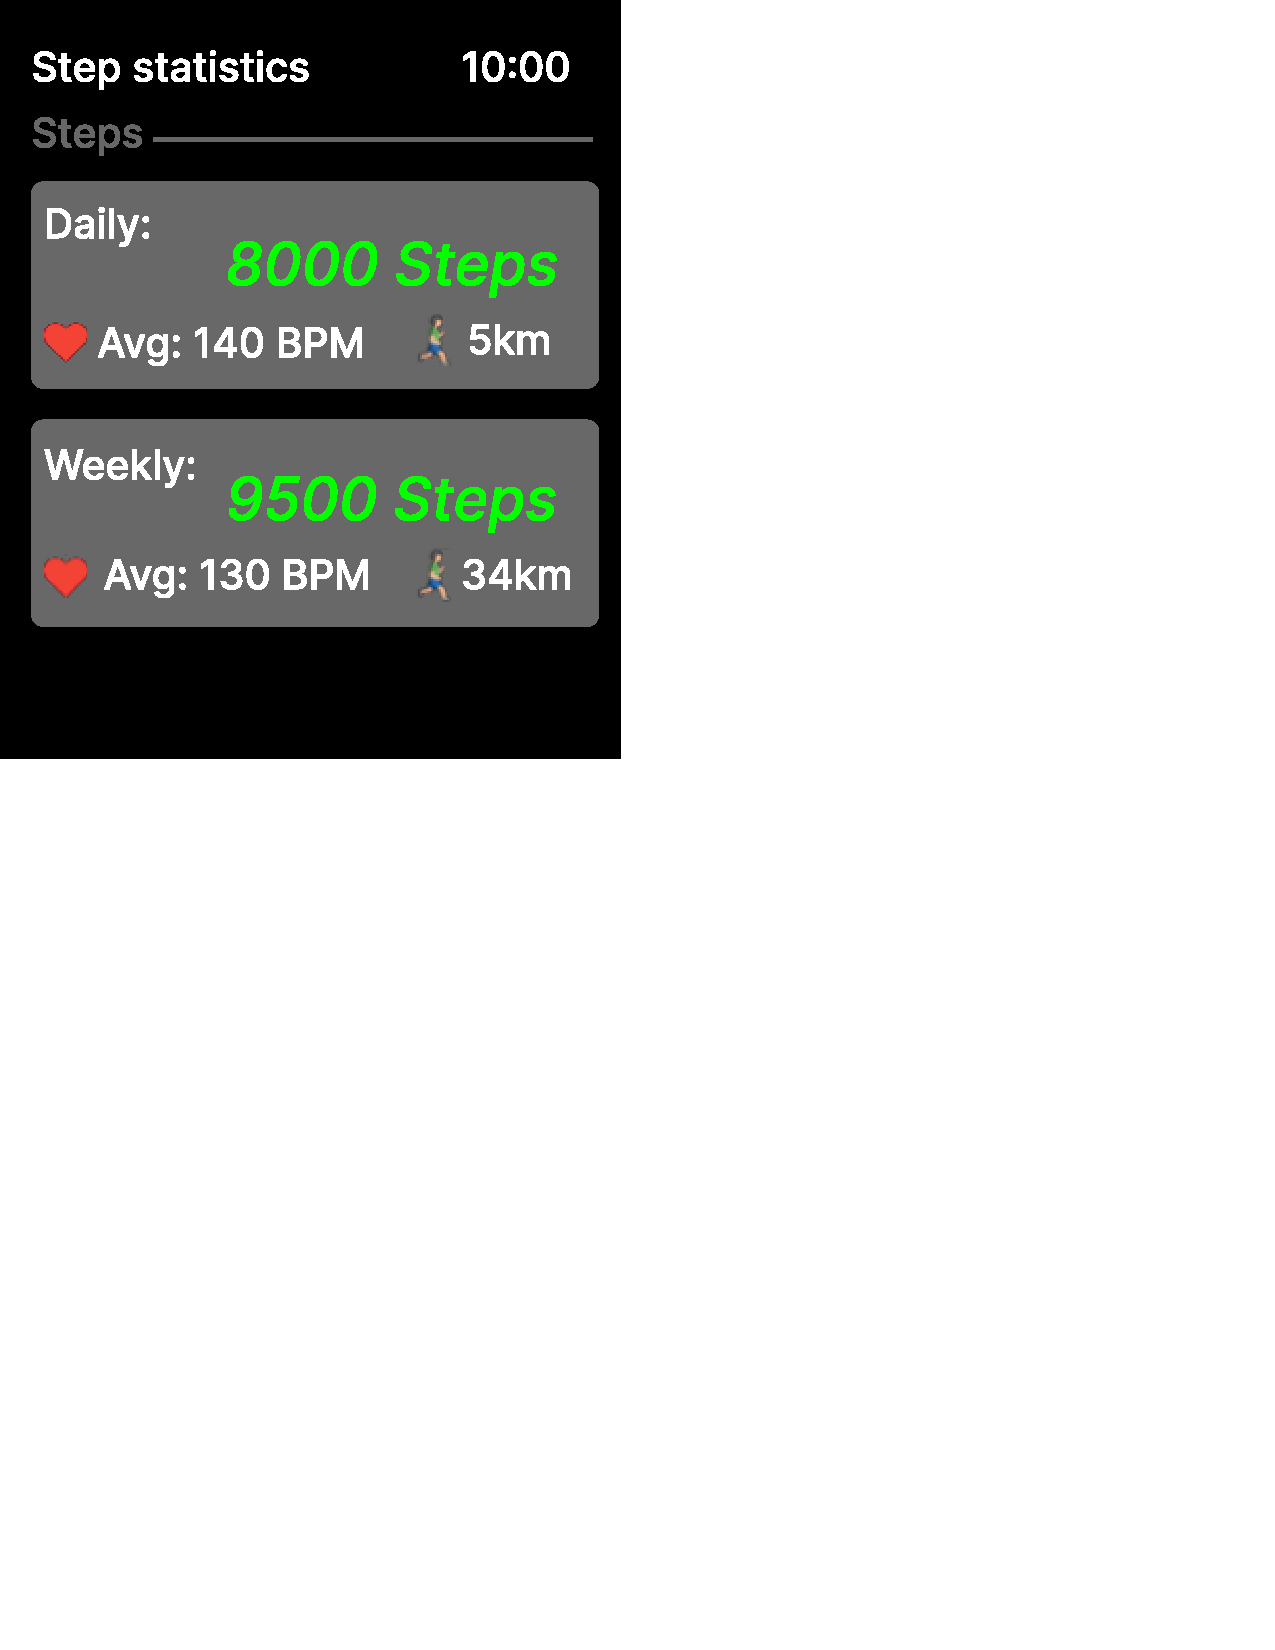
\includegraphics[scale=1.6, angle=0]{Marc/UIPrototype/steps.pdf}
		\end{figure}
		\clearpage
		\begin{figure}[h!]
			\centering
		    	\captionsetup{labelformat=empty}
		    	\caption{Activity Diagram - Calculation and display daily and weekly step count statistics}
		    	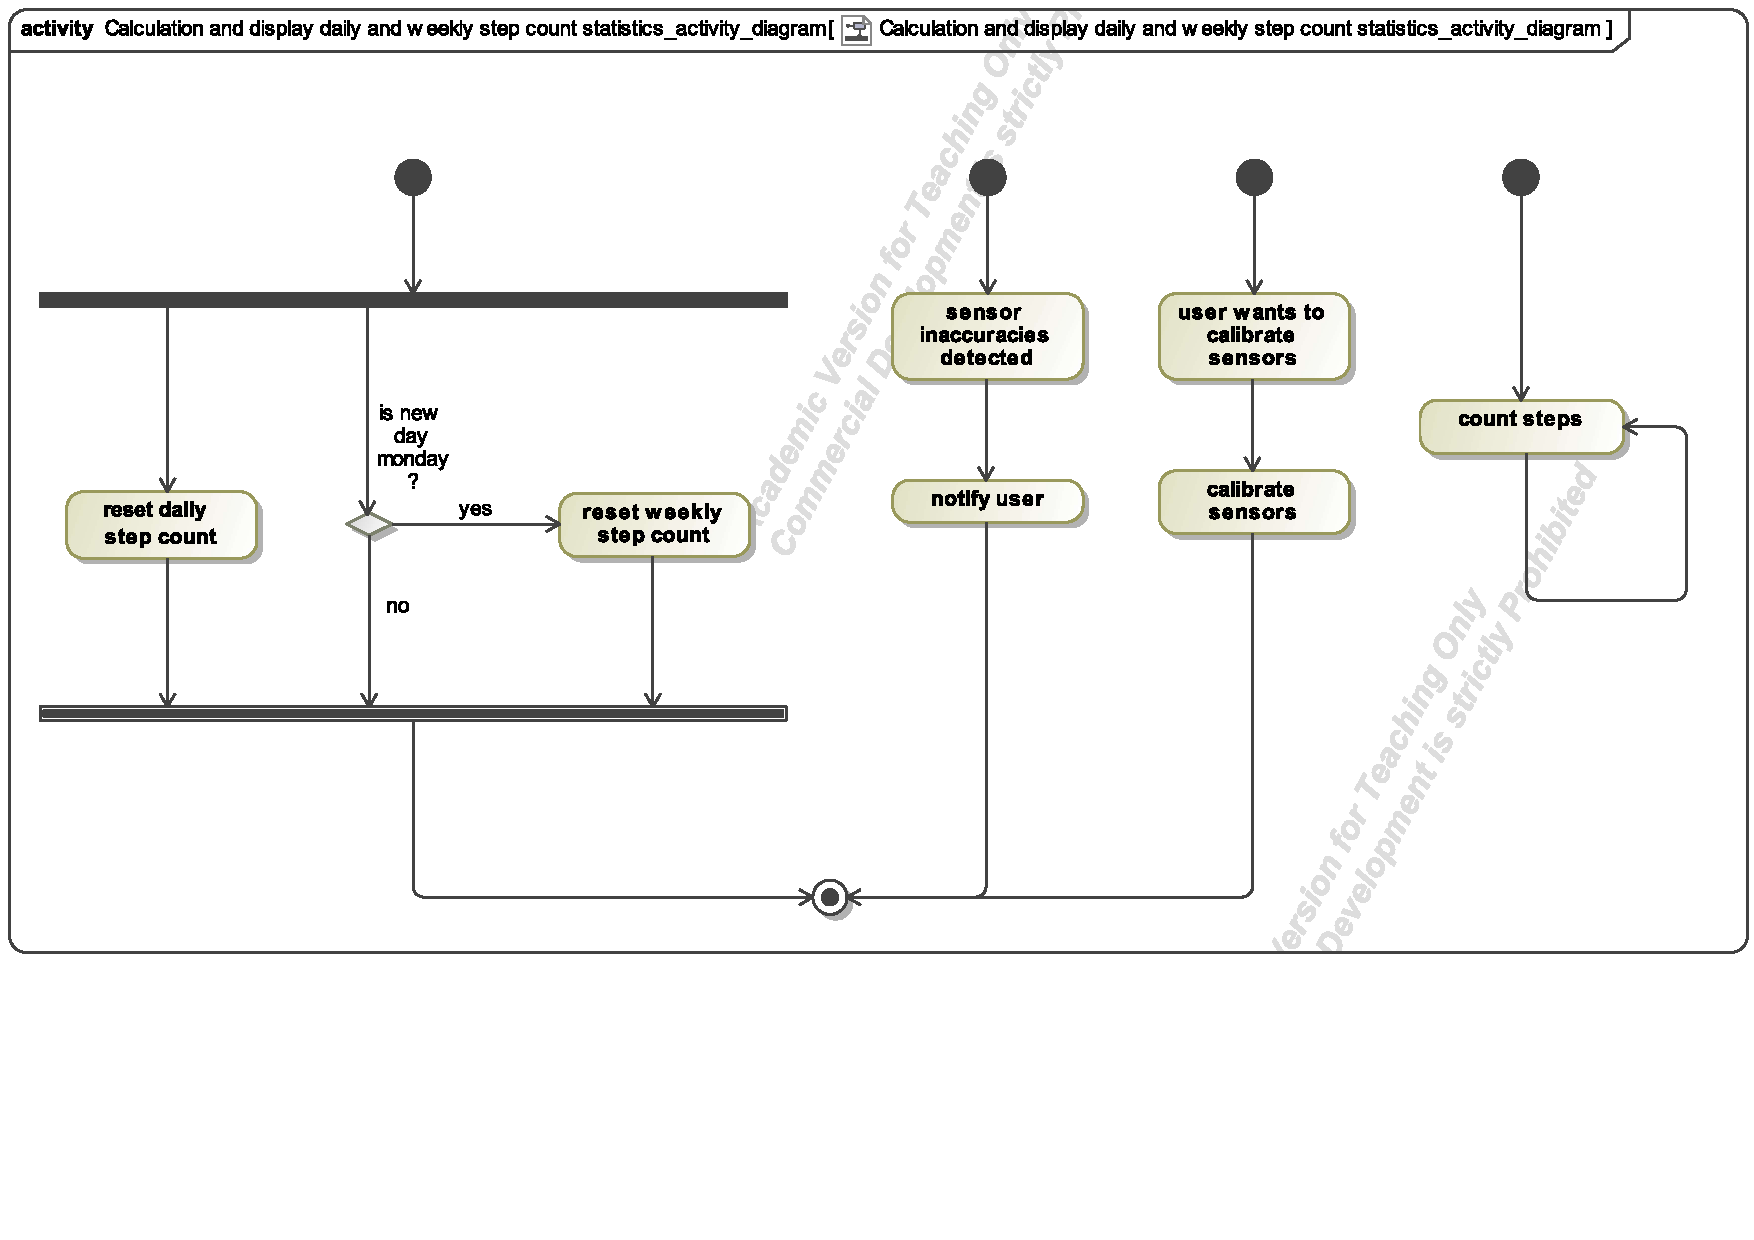
\includegraphics[width=\textwidth, angle=0]{Marc/step/StepCountActivity.pdf}
		\end{figure}
		\clearpage
		\begin{figure}[h!]
			\centering
			\captionsetup{labelformat=empty}
			\caption{UseCase Diagram - Calculation and display daily and weekly step count statistics}
		    	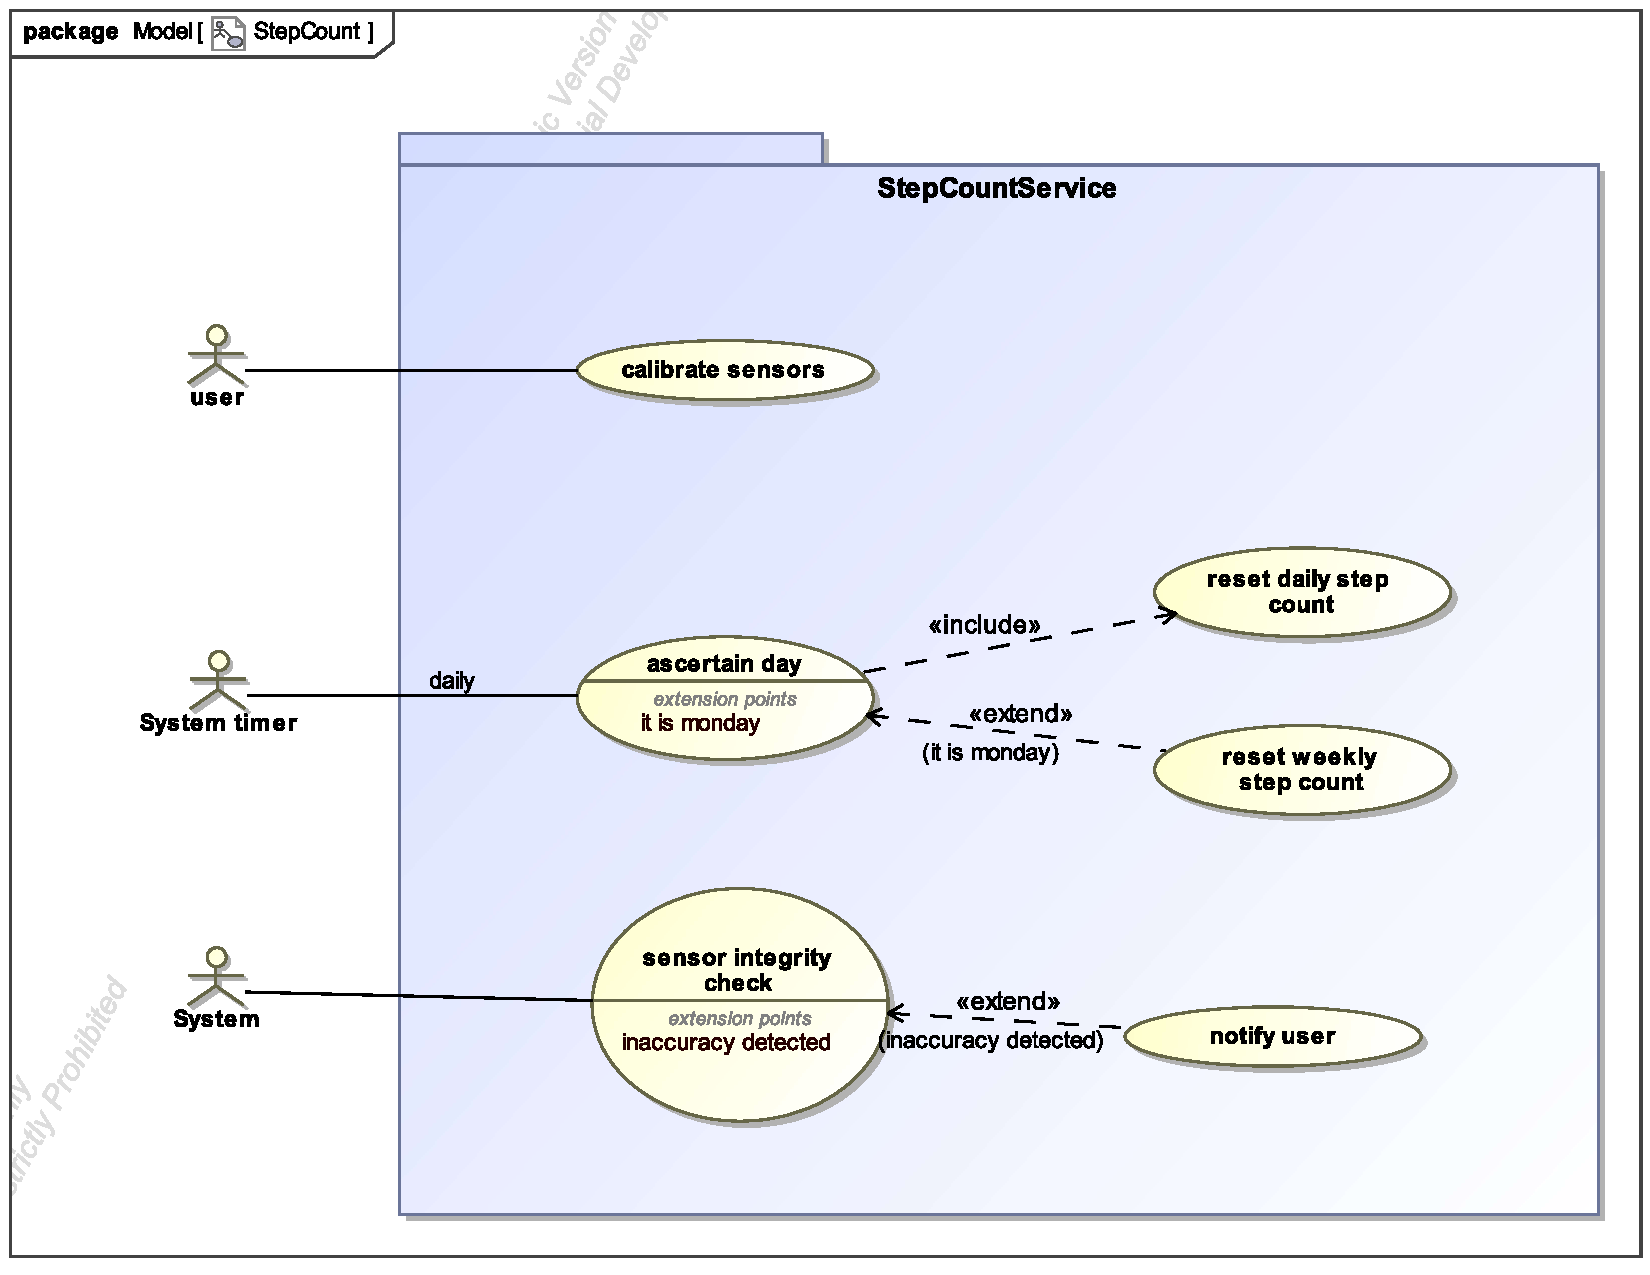
\includegraphics[width=\textwidth, angle=0]{Marc/step/StepCountUseCase.pdf}
		\end{figure}
		\clearpage
		\begin{figure}[h!]
			\centering
			\captionsetup{labelformat=empty}
			\caption{Sequence Diagram - Calculation and display daily and weekly step count statistics}
		    	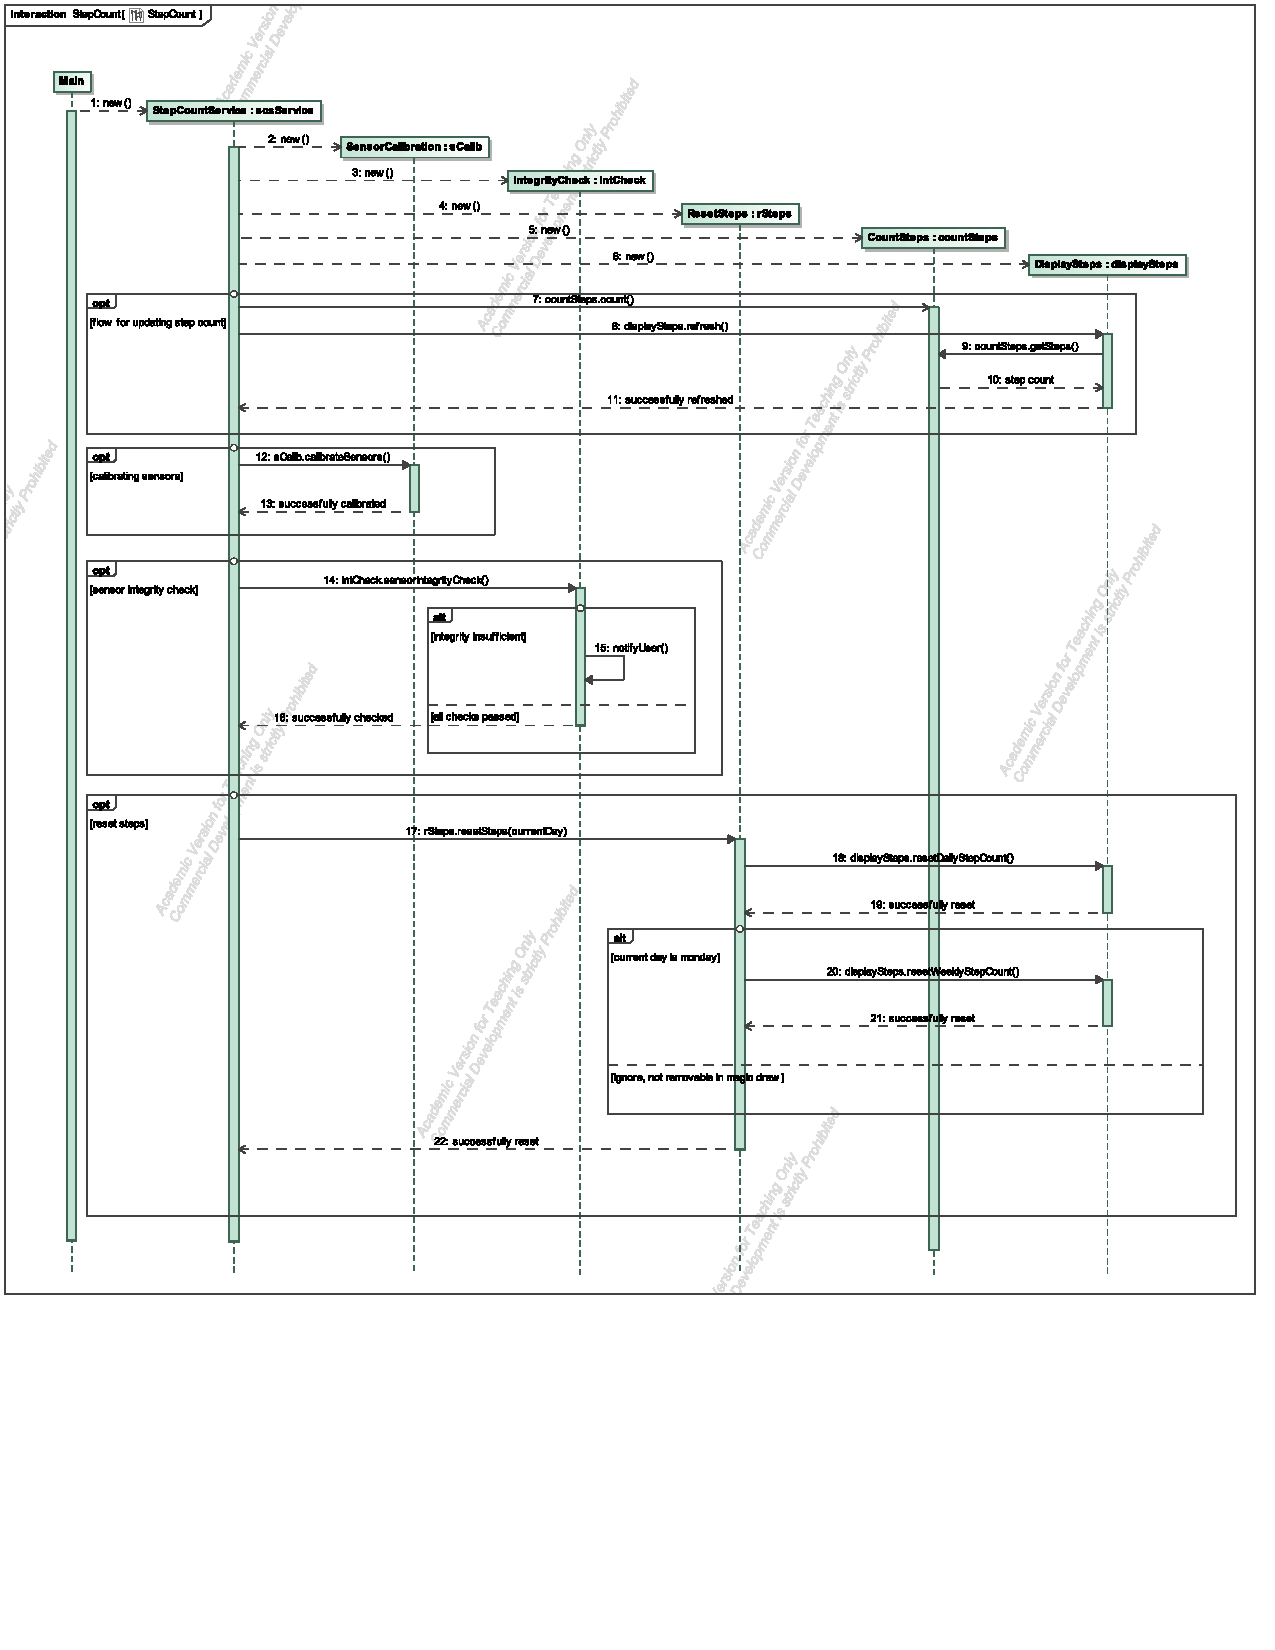
\includegraphics[width=\textwidth, angle=0]{Marc/step/StepCountSequence.pdf}
		\end{figure}
		\clearpage
		\begin{figure}[h!]
			\centering
			\captionsetup{labelformat=empty}
			\caption{Class Diagram - Calculation and display daily and weekly step count statistics}
		    	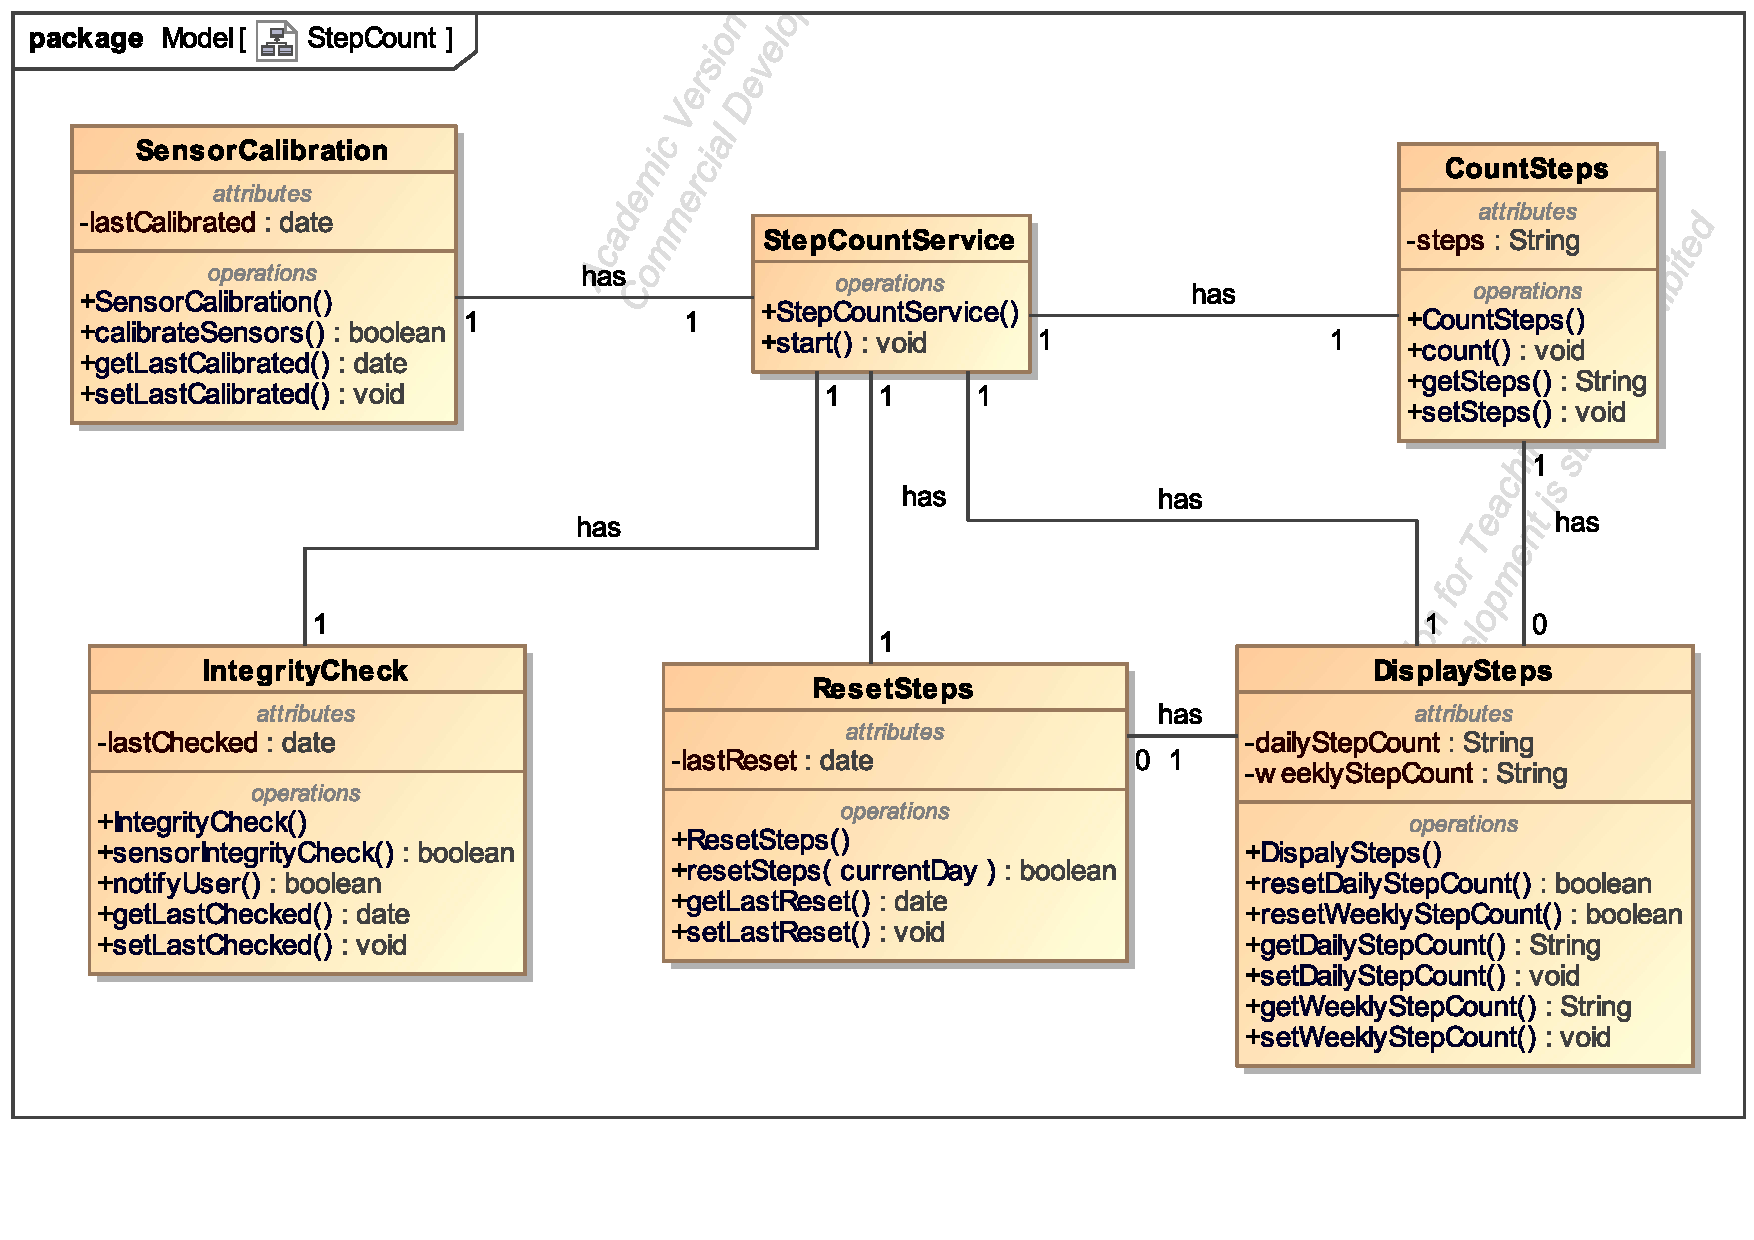
\includegraphics[width=\textwidth, angle=0]{Marc/step/StepCountClass.pdf}
		\end{figure}
		\clearpage

	\subsection{Requirement 10: Create and manages a workout plan}
		\begin{table}[htbp]
			\centering
			\captionsetup{labelformat=empty}
			\caption{UseCase - Create and manages a workout plan}
			\begin{tabularx}{\textwidth}{|>{\raggedright\arraybackslash}p{0.25\textwidth}|X|}
				\hline
				Name             & Create and manages a workout plan                                \\ \hline
				ID               & 10                                                                                       \\ \hline
				Business Value   & Medium                                                                                    \\ \hline
				Description      & A fitness application which allows the user to create and manage personalized workout plans \\ \hline
				Trigger          & Users sets goal in the app and thus triggers the system to generate a personalized plan to reach the goal \\ \hline
				Actors           & User, Fitness app                                 \\ \hline
				Pre-conditions   & The user has installed and registered to the fitness app and the app has access to information about the user's goal                                    \\ \hline
				Post-conditions  & User receives a personalized workout plan                                                         \\ \hline
				Basic Flow       & This is the main scenario where the user gets a personalized workout plan \\ \hline
								 & Actions: \\
								 & 1. The user creates an account and sets his goals. habits and preferences \\
								 & 2. The app configures a customized workout plan specific to the user given information \\
								 & 3. The app provides daily tips and tracks the progress and if the user reached the daily goal \\ \hline
				Alternative Flow A & User can t reach the daily workout goal because of personal circumstances \\
								 & Actions: \\
								 & 1. The app gives the user the possibility to create a new plan for the following day which contain a change of the exercise sets so the user can catch up the missed ones \\
								 & 2. The user adapts the new plan for the following day and after that day the plan continuous normally \\ \hline
				Alternative Flow B & The plan doesn't fit anymore because of physical changes \\
								 & Actions: \\
								 & 1. The app goes with the plan but user isn't satisfied because of changes e.g. weight gain or loss \\
								 & 2. The app offers every month a feedback sheet so the user can fill in every changes \\
								 & 3. The app does a new goal calculation and creates a new workout plan in the likening of the user \\ \hline
			\end{tabularx}
		\end{table}
		\paragraph{Functional requirements}
		\begin{itemize}
			\item The System should accurately calculate the total numbers of steps taken by the user based on the given data from the application
			\item User should be able to view a step count statistic for the day and a weekly breakdown		
		\end{itemize}
		
		\paragraph{Non-functional requirements}
		\begin{itemize}
			\item The System has to process and update the step count data in real time to ensure that the user get the newest information at any time
			\item The system has to handle the increasing step data without decreasing the performance Quality
		\end{itemize}
		\clearpage
		\begin{figure}[h!]
			\centering
			\captionsetup{labelformat=empty}
		    	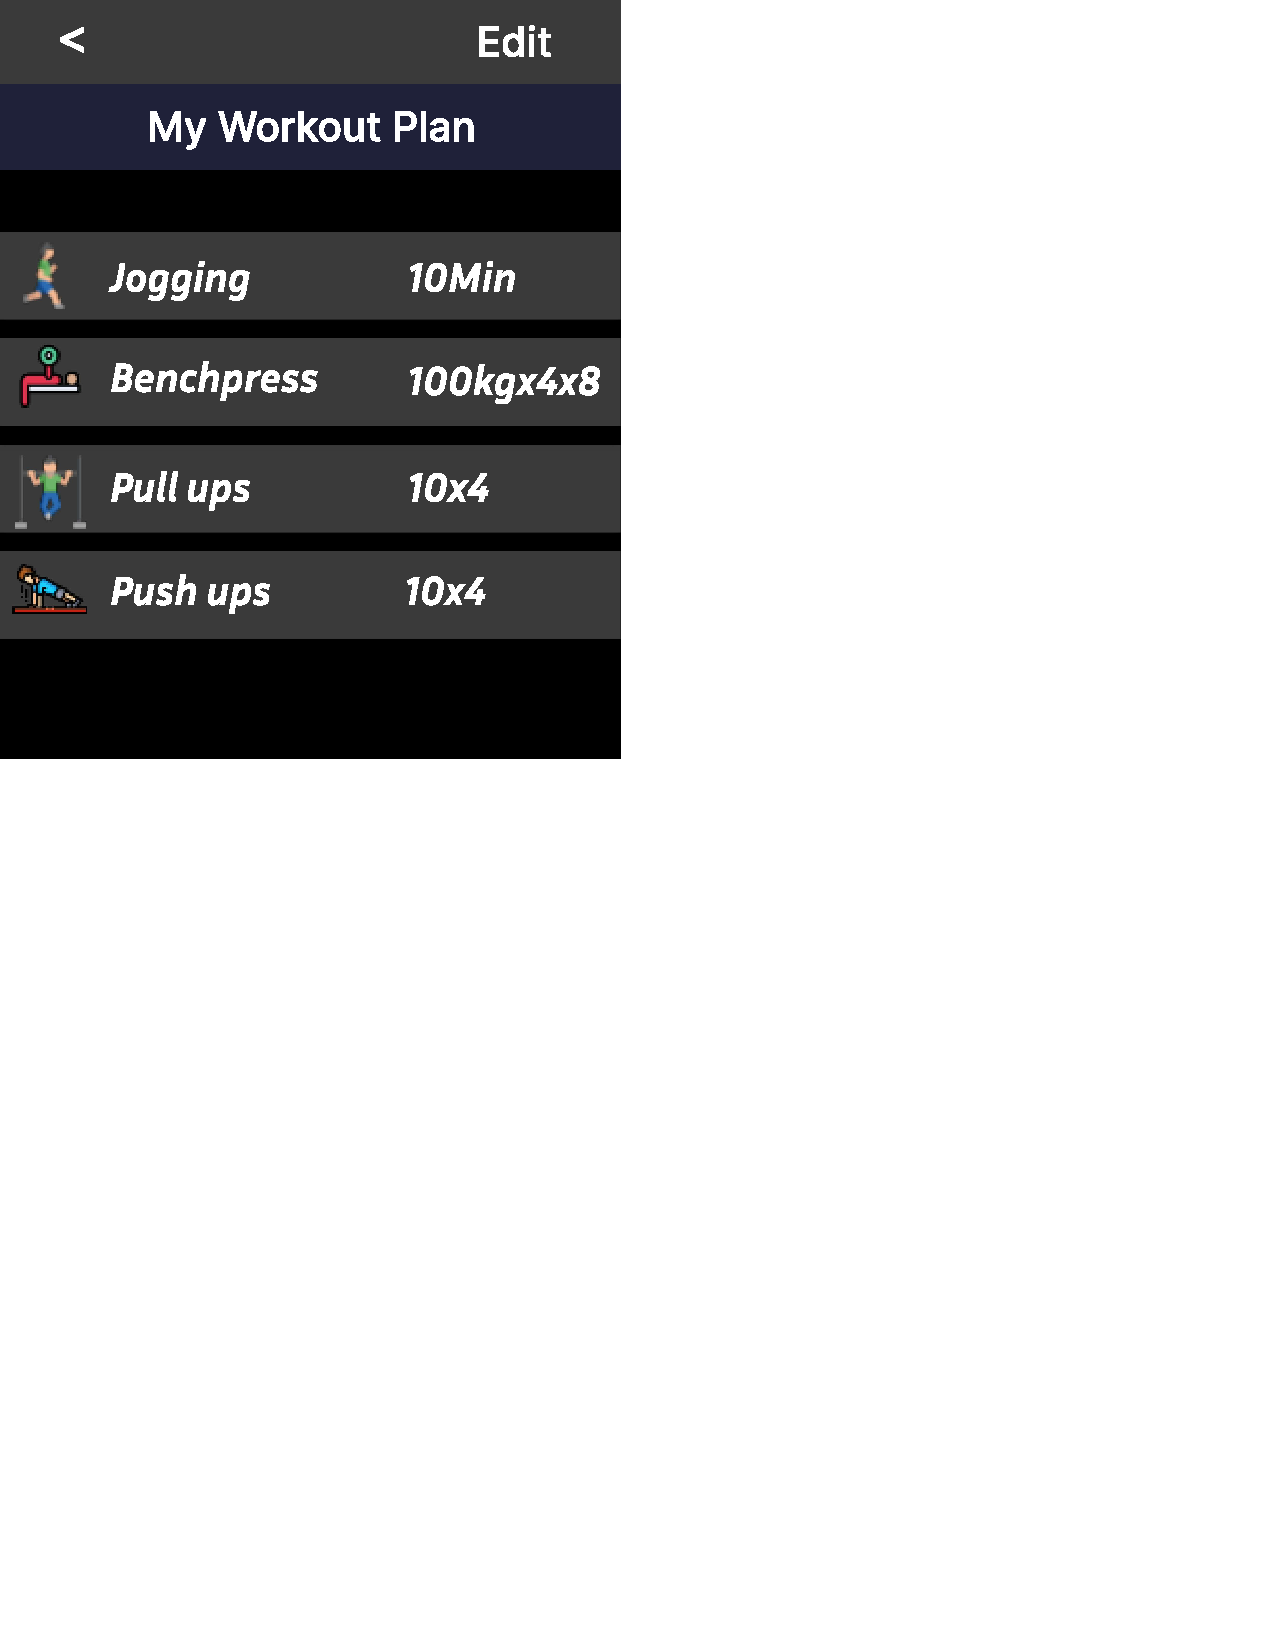
\includegraphics[scale=1.6, angle=0]{Marc/UIPrototype/workout.pdf}
			\caption{UI Prototype - Create and manages a workout plan}
		\end{figure}
		\clearpage
		\begin{figure}[h!]
		    	\centering
		   	\captionsetup{labelformat=empty}
		   	\caption{Activity Diagram - Create and manages a workout plan}
		    	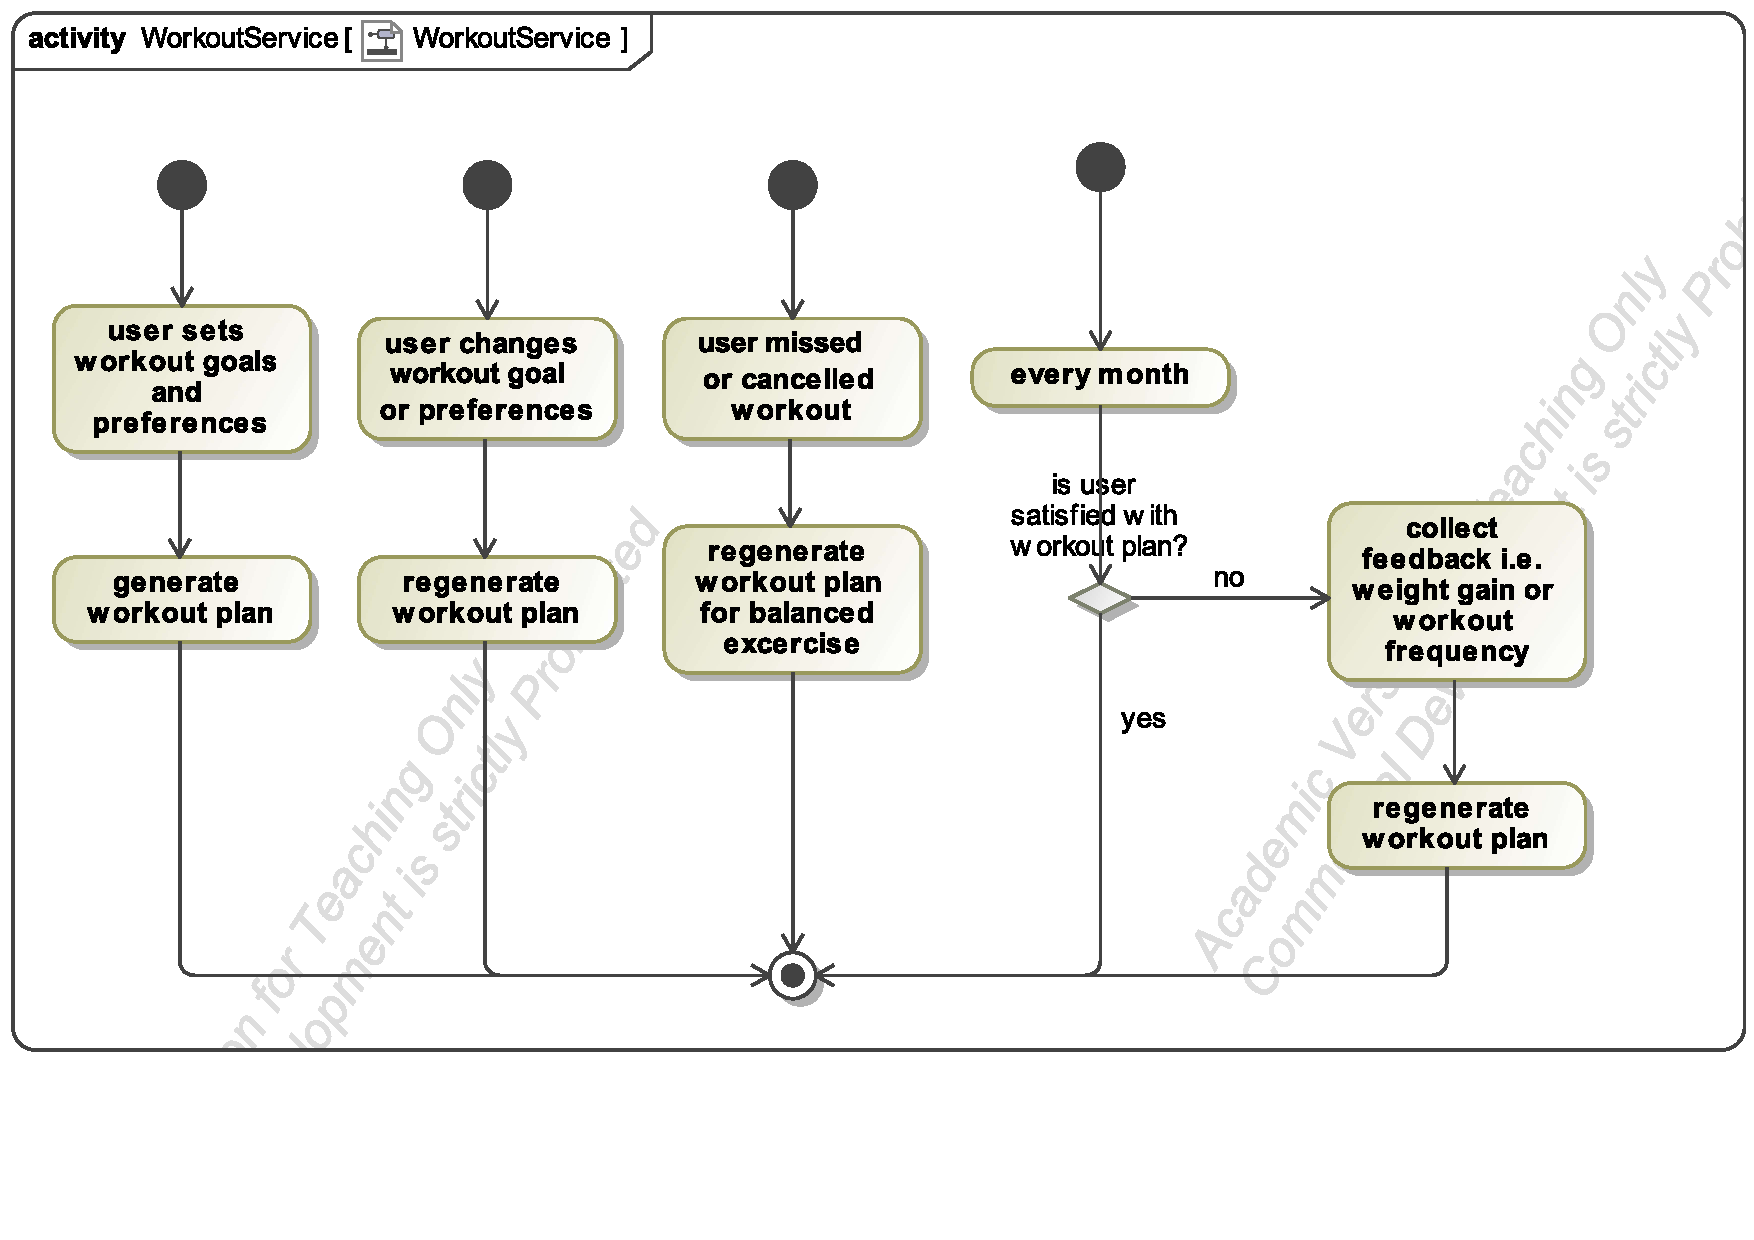
\includegraphics[width=\textwidth, angle=0]{Marc/workout/WorkoutServiceActivity.pdf}
		\end{figure}
		\clearpage
		\begin{figure}[h!]
			\centering
			\captionsetup{labelformat=empty}
			\caption{UseCase Diagram - Create and manages a workout plan}
		    	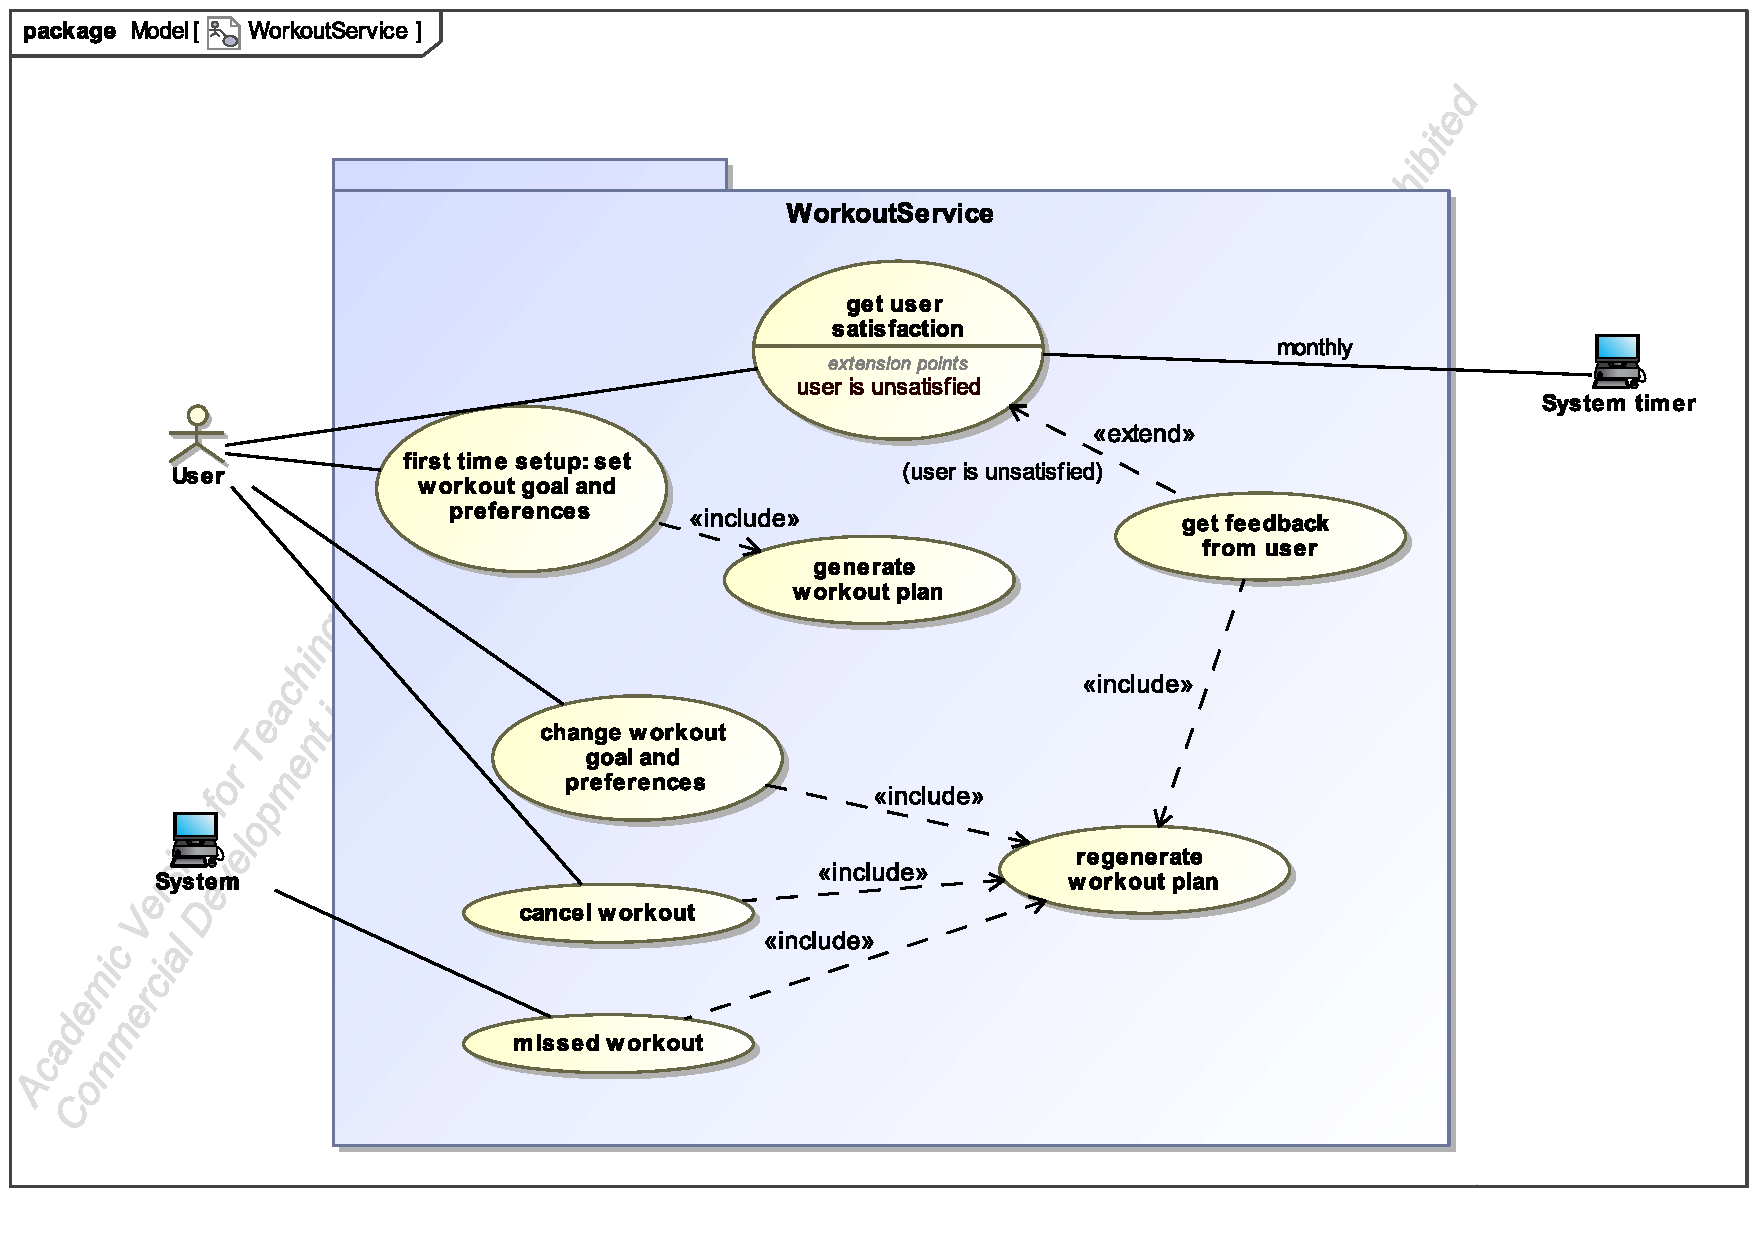
\includegraphics[width=\textwidth, angle=0]{Marc/workout/WorkoutServiceUseCase.pdf}
		\end{figure}
		\clearpage
		\begin{figure}[h!]
			\centering
			\captionsetup{labelformat=empty}
			\caption{Sequence Diagram - Create and manages a workout plan}
		    	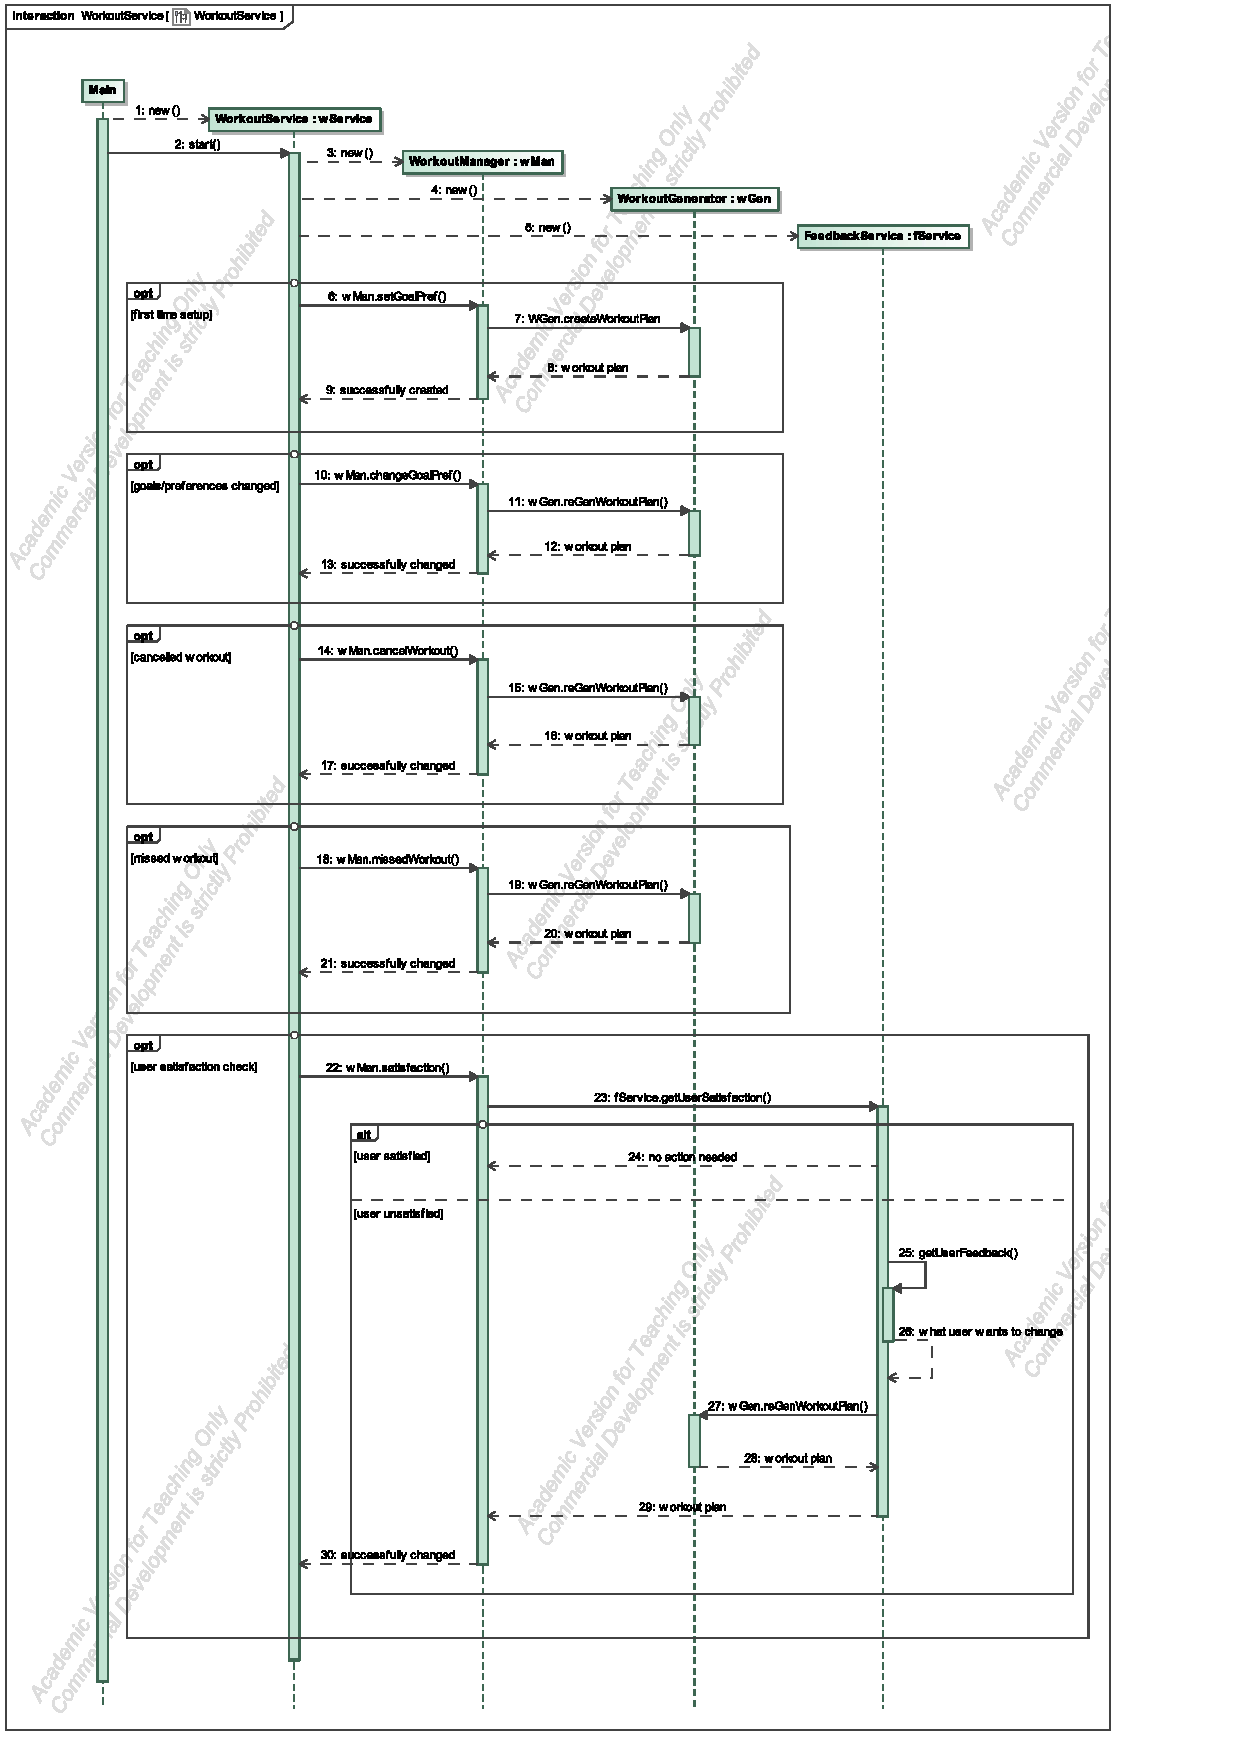
\includegraphics[scale=0.75, angle=0]{Marc/workout/WorkoutServiceSequence.pdf}
		\end{figure}
		\clearpage
		\begin{figure}[h!]
			\centering
			\captionsetup{labelformat=empty}
			\caption{Class Diagram - Create and manages a workout plan}
		    	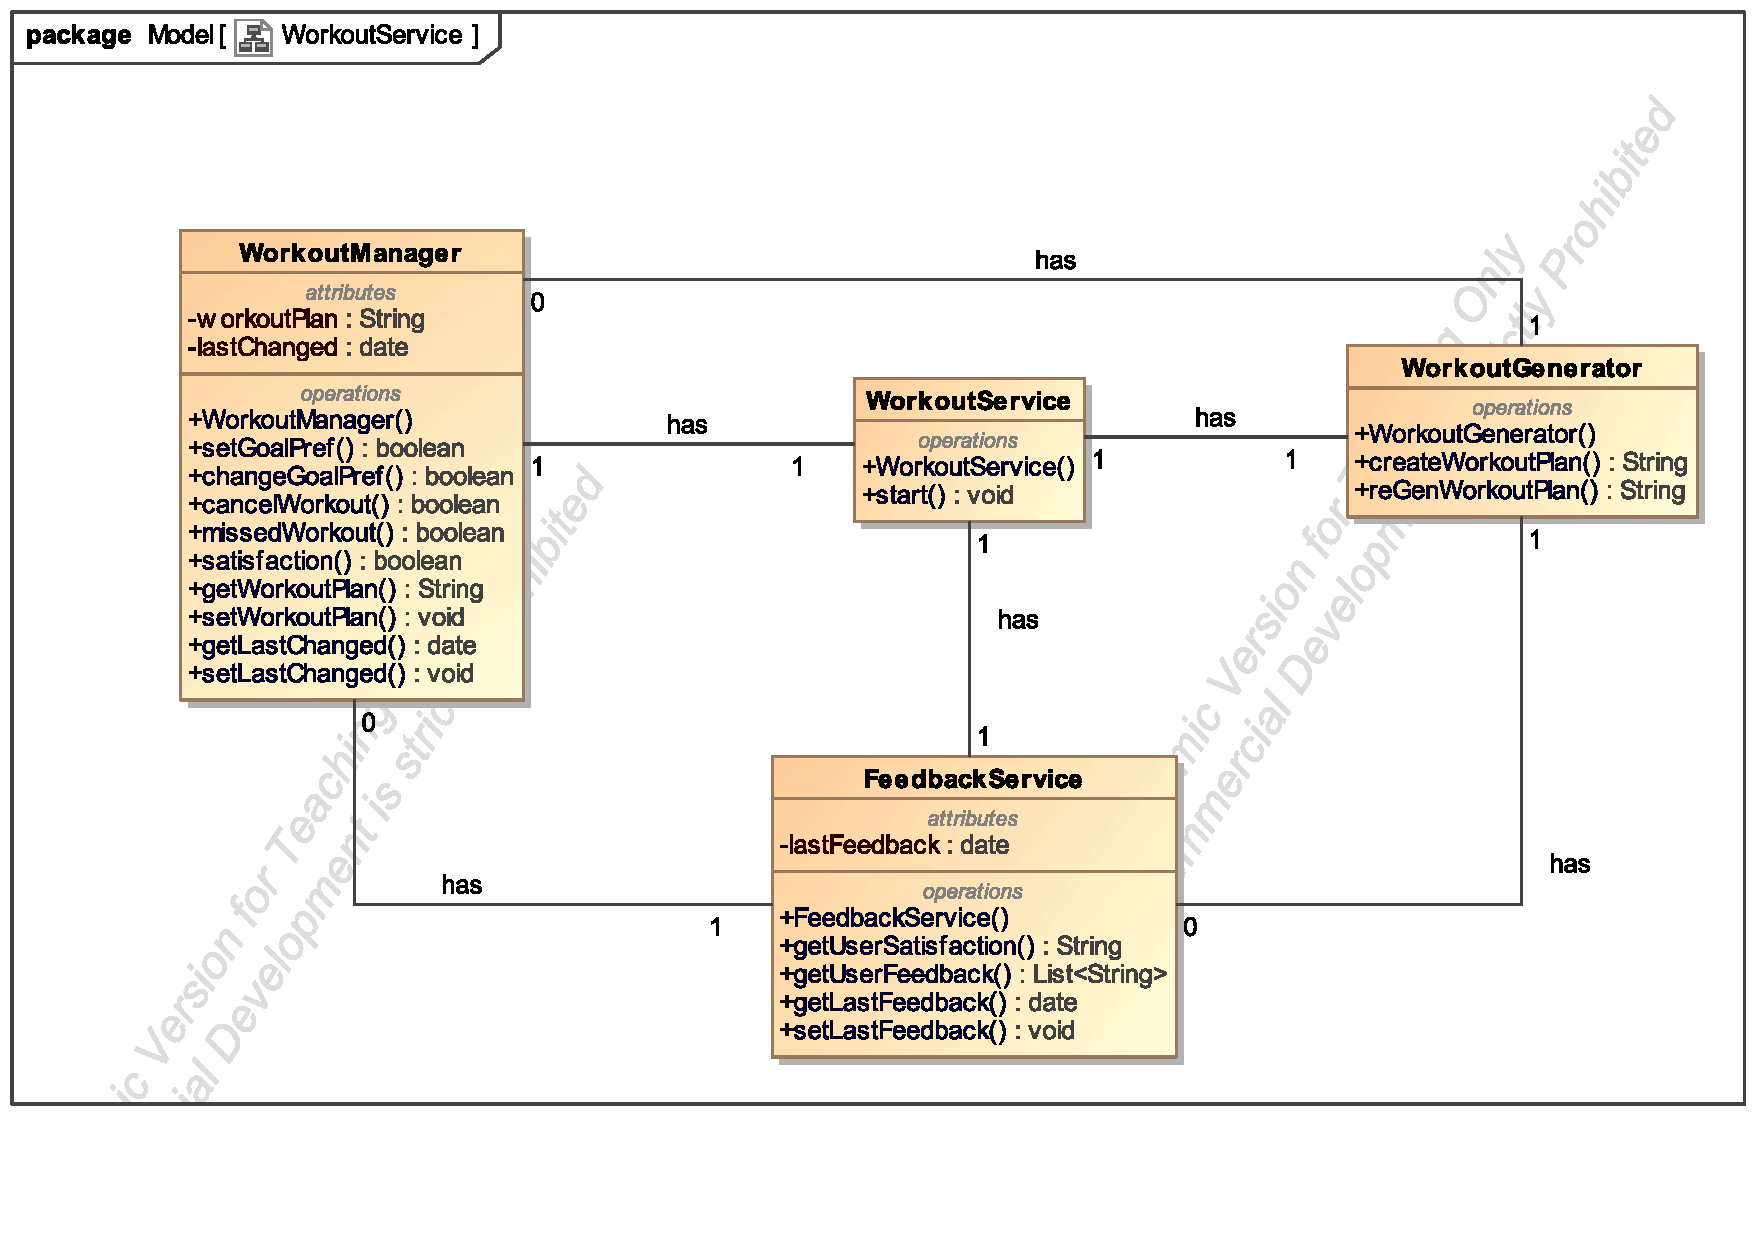
\includegraphics[width=\textwidth, angle=0]{Marc/workout/WorkoutServiceClass.pdf}
		\end{figure}
		\clearpage

	\subsection{Requirement 21: Race time prediction}
		\begin{table}[htbp]
			\centering
			\captionsetup{labelformat=empty}
			\caption{UseCase - Race time prediction}
			\begin{tabularx}{\textwidth}{|>{\raggedright\arraybackslash}p{0.25\textwidth}|X|}
				\hline
				Name             & Race time prediction                                \\ \hline
				ID               & 21                                                                                       \\ \hline
				Business Value   & Low                                                                                    \\ \hline
				Description      & Predicts the time it will take to finish a certain challenge depending on previous performance \\ \hline
				Trigger          & When user selects a workout or route \\ \hline
				Actors           & User, smart watch                                 \\ \hline
				Pre-conditions   & User accepted historical data and selects a workout routine or route                                    \\ \hline
				Post-conditions  & Historical data gets updated on current performance                                                         \\ \hline
				Basic Flow       & This is the main scenario where the user accepted historical data and is connected to the internet \\ \hline
								 & Actions: \\
								 & 1. The smartwatch calculates how long a certain activity takes the user to do, from historical data \\
								 & 2. User can opt out of this service \\
								 & 3. User can reset historical data \\ \hline
				Alternative Flow A & The User didn't accept historical data collection or opted out of this service \\
								 & Actions: \\
								 & 1. Smartwatch calculates an estimate depending on global average \\
								 & 2. User has the option to opt in again \\ \hline
				Alternative Flow B & Not enough historical data found to calculate prediction or data is corrupted \\
								 & Actions: \\
								 & 1. Smartwatch calculates an estimate from backup \\
								 & 2. Smartwatch notifies the user about the problem \\ \hline
			\end{tabularx}
		\end{table}
		\paragraph{Functional requirements}
		\begin{itemize}
			\item The system should accurately calculate the time based on the given data from the application
			\item The system should have calculated the time already before it is displayed for a seamless experience	
		\end{itemize}
		
		\paragraph{Non-functional requirements}
		\begin{itemize}
			\item The system has to update the calculated time before a workout to ensure that the user get the newest information
			\item The system has to be able to adapt to missing data or corrupted data
		\end{itemize}
		\clearpage
		\begin{figure}[h!]
		    	\centering
		   	\captionsetup{labelformat=empty}
		   	\caption{Activity Diagram - Race time prediction}
		    	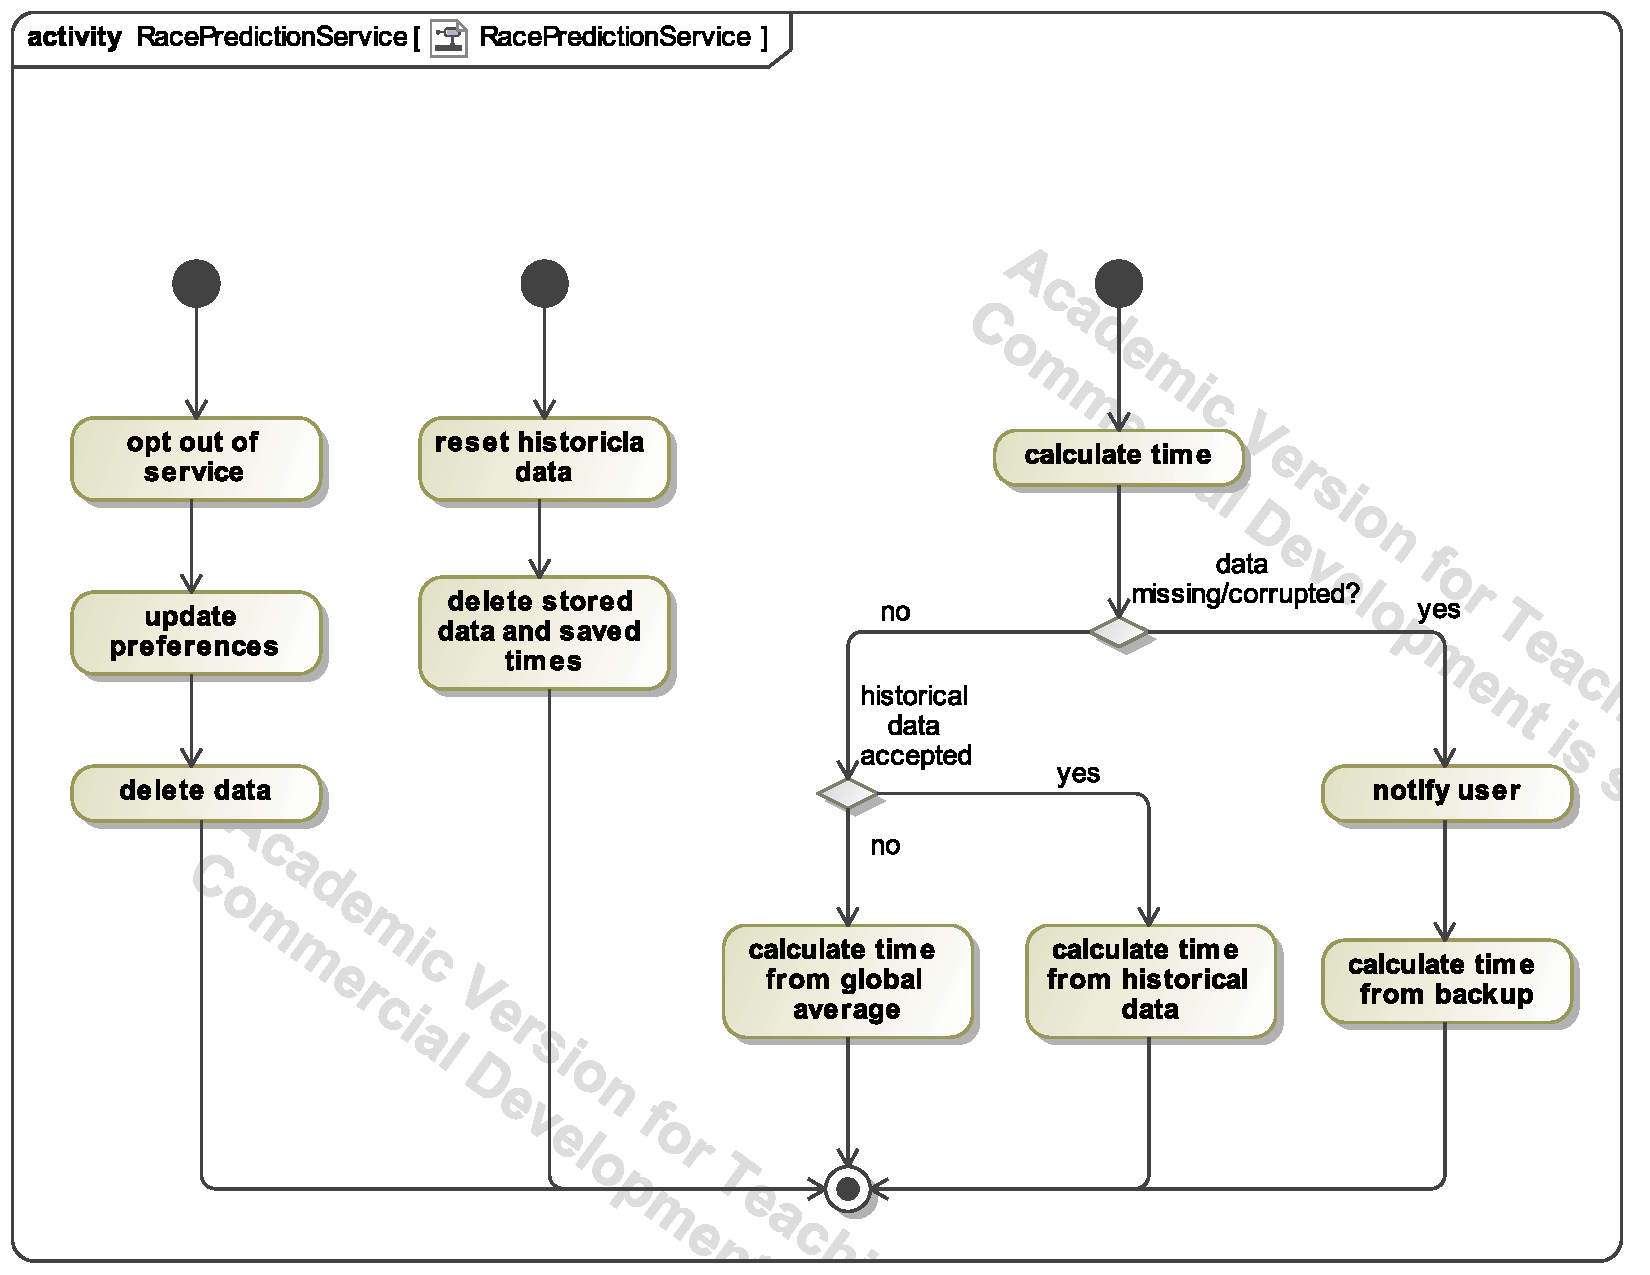
\includegraphics[width=\textwidth, angle=0]{Marc/race/RacePredictionServiceActivity.pdf}
		\end{figure}
		\clearpage
		\begin{figure}[h!]
			\centering
			\captionsetup{labelformat=empty}
			\caption{UseCase Diagram - Race time prediction}
		    	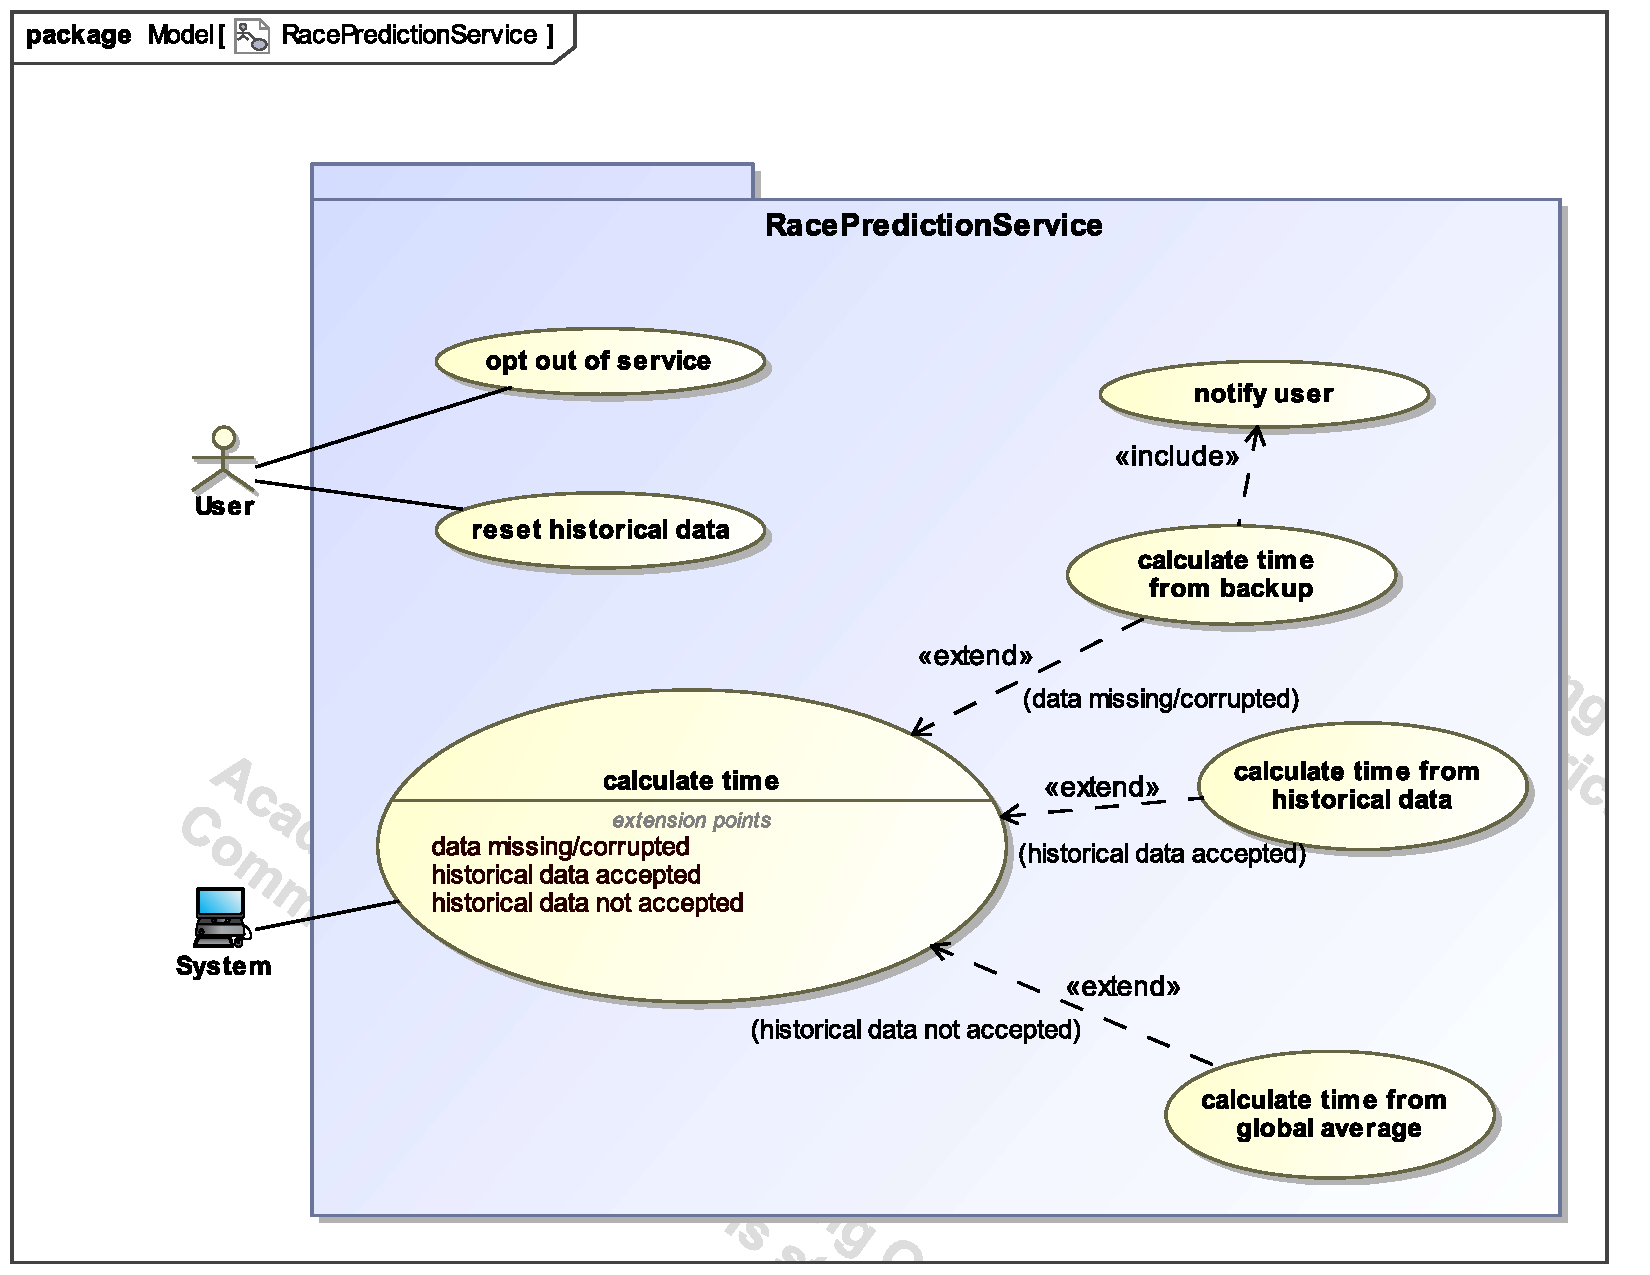
\includegraphics[width=\textwidth, angle=0]{Marc/race/RacePredictionServiceUseCase.pdf}
		\end{figure}
		\clearpage
		\begin{figure}[h!]
			\centering
			\captionsetup{labelformat=empty}
			\caption{Sequence Diagram - Race time prediction}
		    	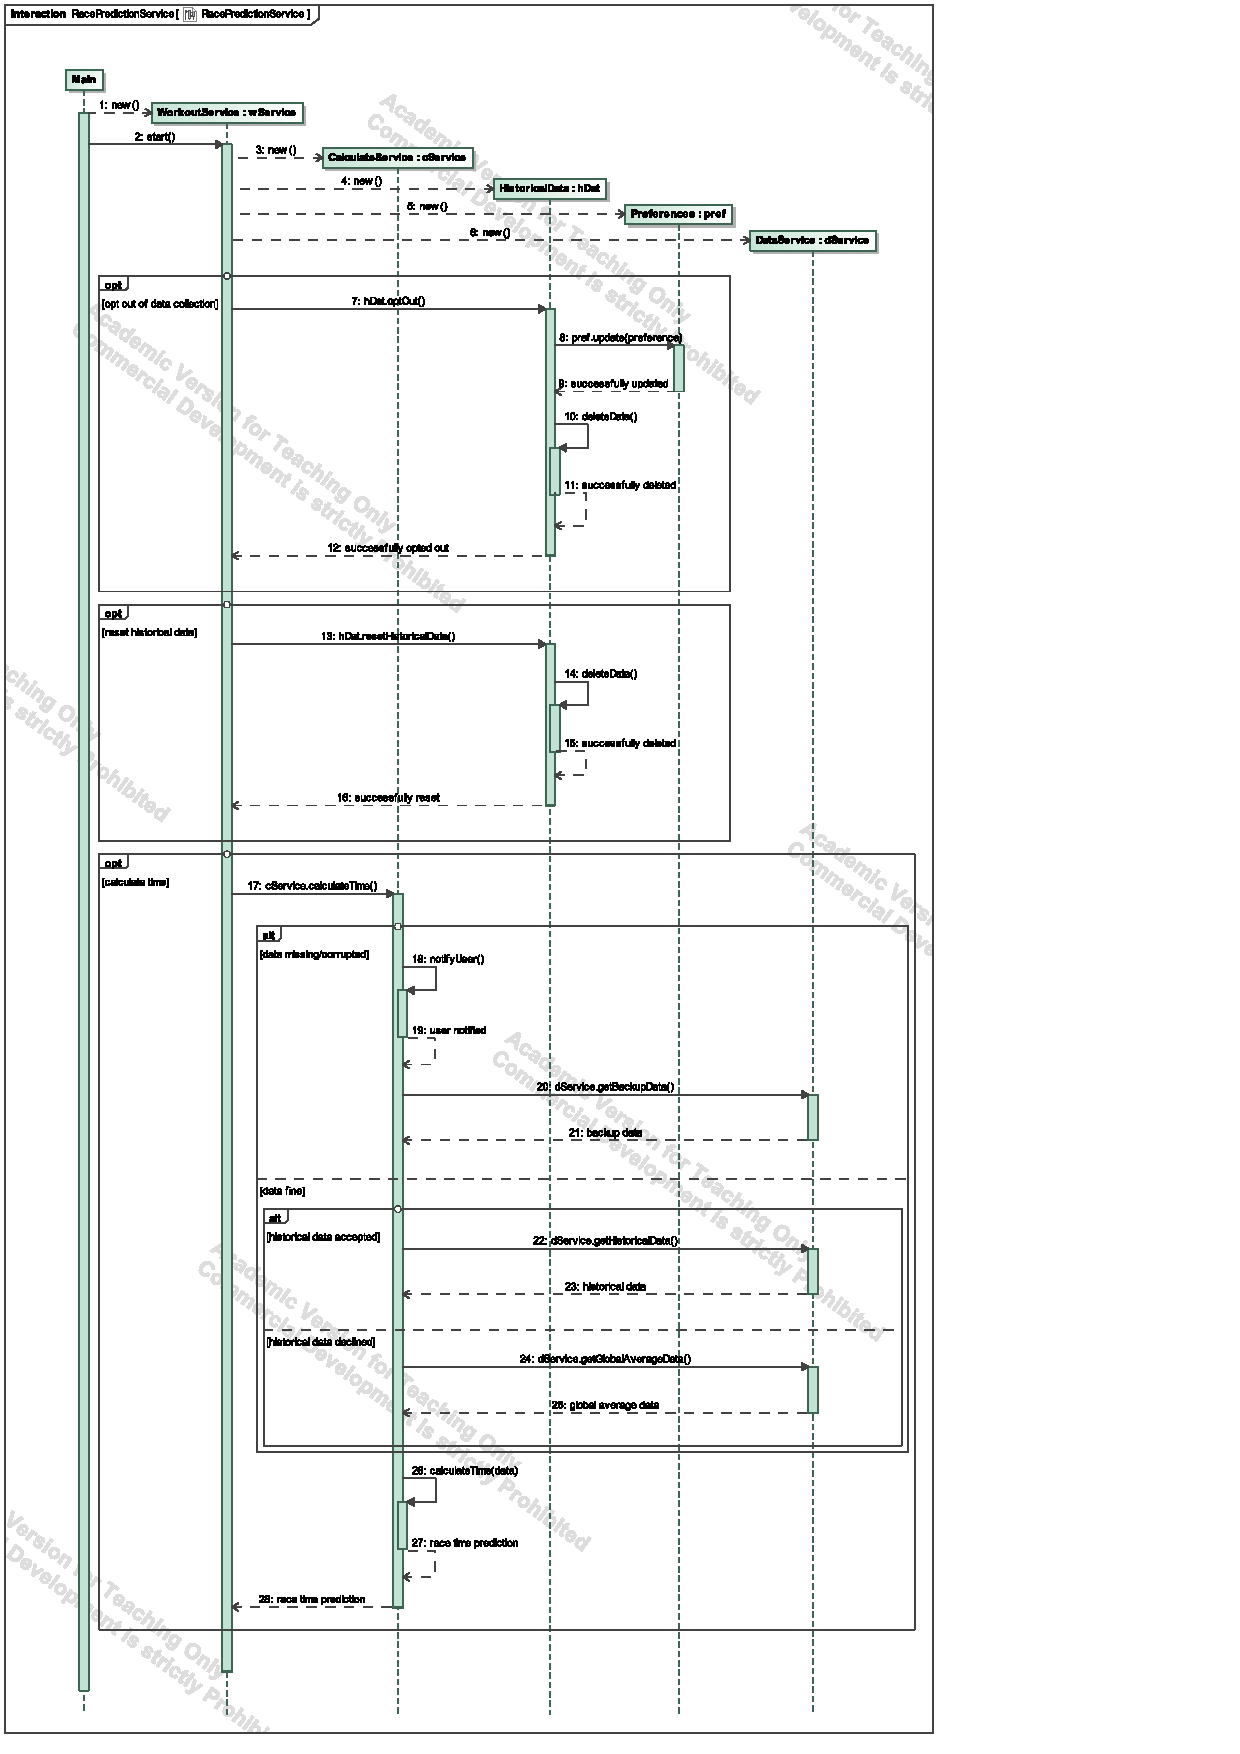
\includegraphics[scale=0.75, angle=0]{Marc/race/RacePredictionServiceSequence.pdf}
		\end{figure}
		\clearpage
		\begin{figure}[h!]
			\centering
			\captionsetup{labelformat=empty}
			\caption{Class Diagram - Race time prediction}
		    	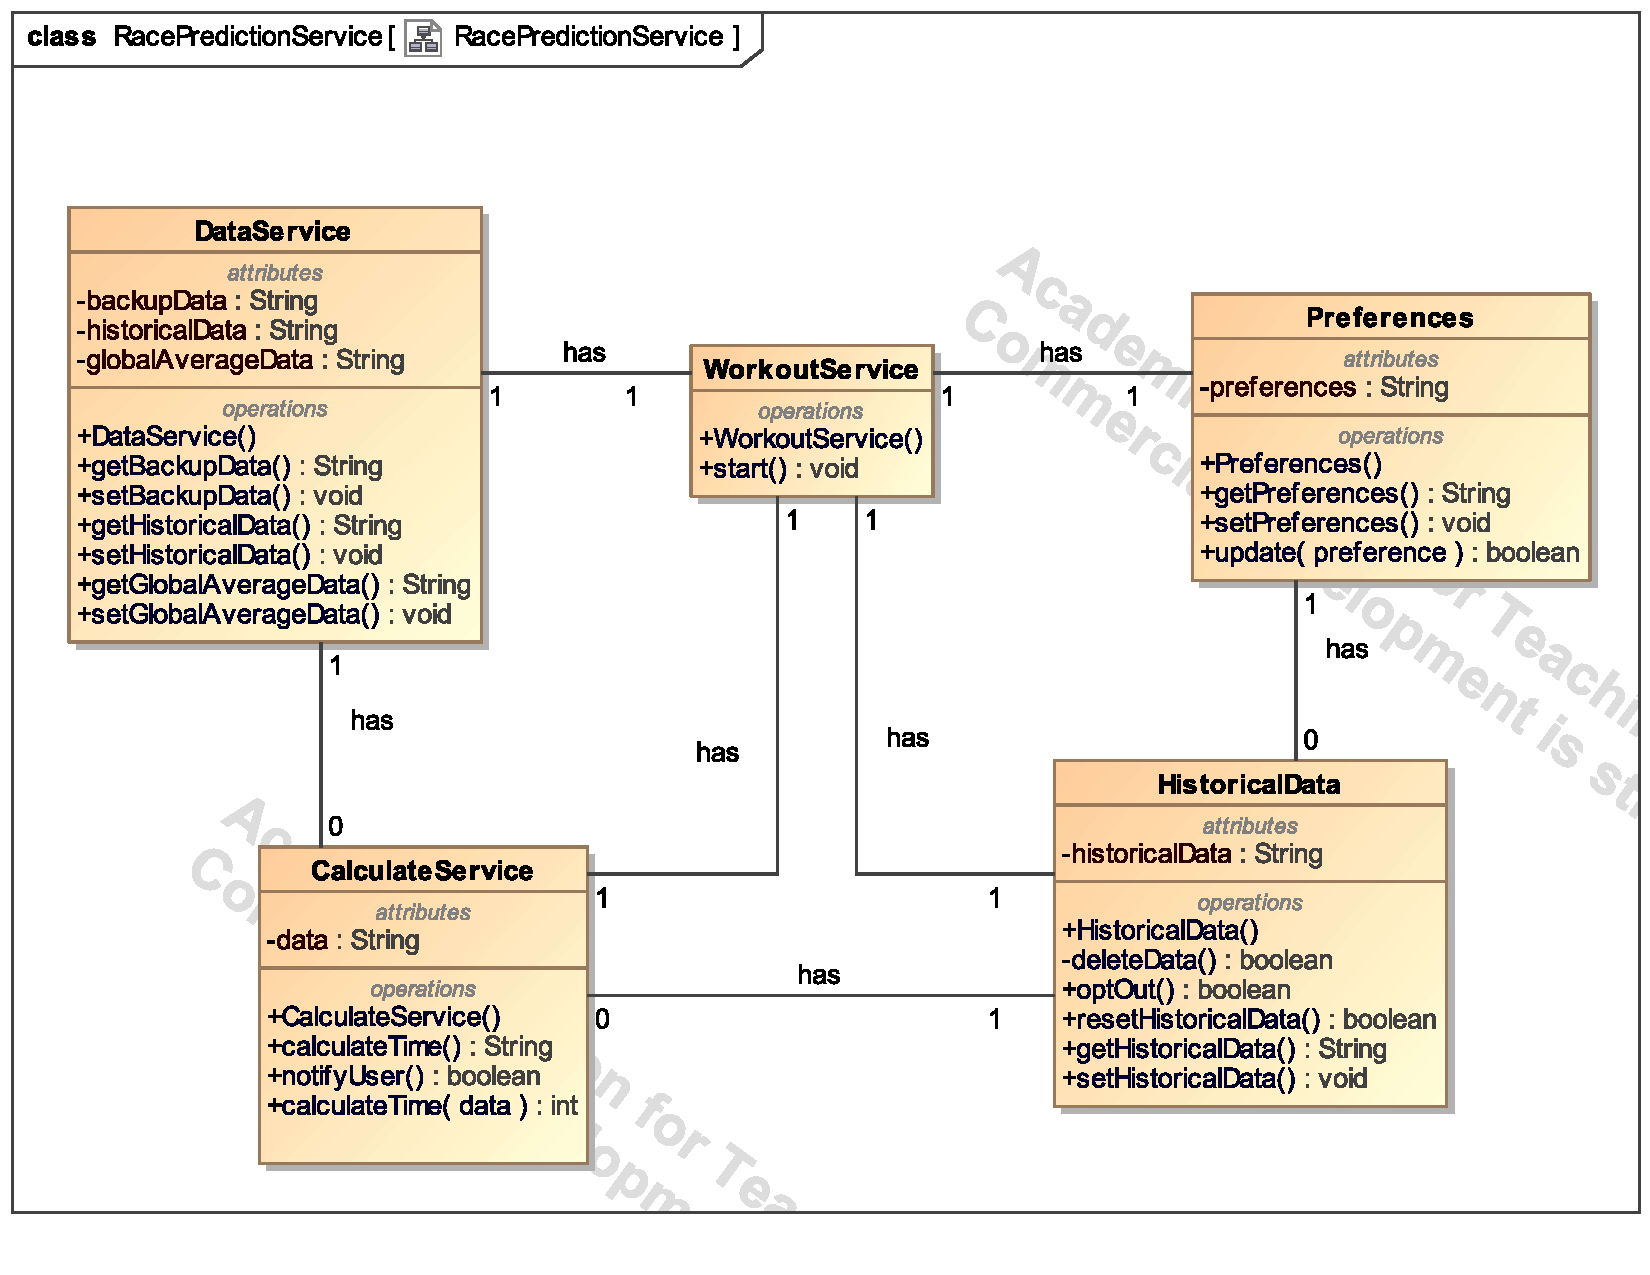
\includegraphics[width=\textwidth, angle=0]{Marc/race/RacePredictionServiceClass.pdf}
		\end{figure}
		\clearpage	

	\subsection{Requirement 22: light detection for brightness (light sensor)}
		\begin{table}[htbp]
			\centering
			\captionsetup{labelformat=empty}
			\caption{UseCase - light detection for brightness (light sensor)}
			\begin{tabularx}{\textwidth}{|>{\raggedright\arraybackslash}p{0.25\textwidth}|X|}
				\hline
				Name             & light detection for brightness (light sensor)                                \\ \hline
				ID               & 22                                                                                       \\ \hline
				Business Value   & Low                                                                                    \\ \hline
				Description      & Adjusts brightness of the screen depending on ambient light \\ \hline
				Trigger          & Changes in ambient light detected \\ \hline
				Actors           & smart watch                                 \\ \hline
				Pre-conditions   & light sensor/camera not deactivated, user activated auto-brightness                                    \\ \hline
				Post-conditions  & Brightness is adjusted                                                         \\ \hline
				Basic Flow       & This is the main scenario the brightness gets adjusted based on ambient light \\ \hline
								 & Actions: \\
								 & 1. Smartwatch detects ambient light \\
								 & 2. Smartwatch adjusts brightness accordingly \\ \hline
				Alternative Flow A & Sensor gets covered completely \\
								 & Actions: \\
								 & 1. Smartwatch goes into idle mode \\
								 & 2. Smartwatch makes a closing sound \\ \hline
				Alternative Flow B & When smartwatch detects flashing lights it enters party mode flashing random colors on screen \\
								 & Actions: \\
								 & 1. Smartwatch detects flashing lights \\
								 & 2. Smartwatch plays fun animation \\ 
								 & 3. User can turn this off \\ \hline
			\end{tabularx}
		\end{table}
		\paragraph{Functional requirements}
		\begin{itemize}
			\item The system should accurately calculate the brightness based on the given data from the sensor
			\item The system should calculate the brightness every few seconds to save battery
			\item The system should go into idle mode when the sensor gets covered
		\end{itemize}
		
		\paragraph{Non-functional requirements}
		\begin{itemize}
			\item The system should flash lights back when a party is detected
			\item The system has to be able withstand bright light
		\end{itemize}
		\clearpage
		\begin{figure}[h!]
		    	\centering
		   	\captionsetup{labelformat=empty}
		   	\caption{Activity Diagram - light detection for brightness (light sensor)}
		    	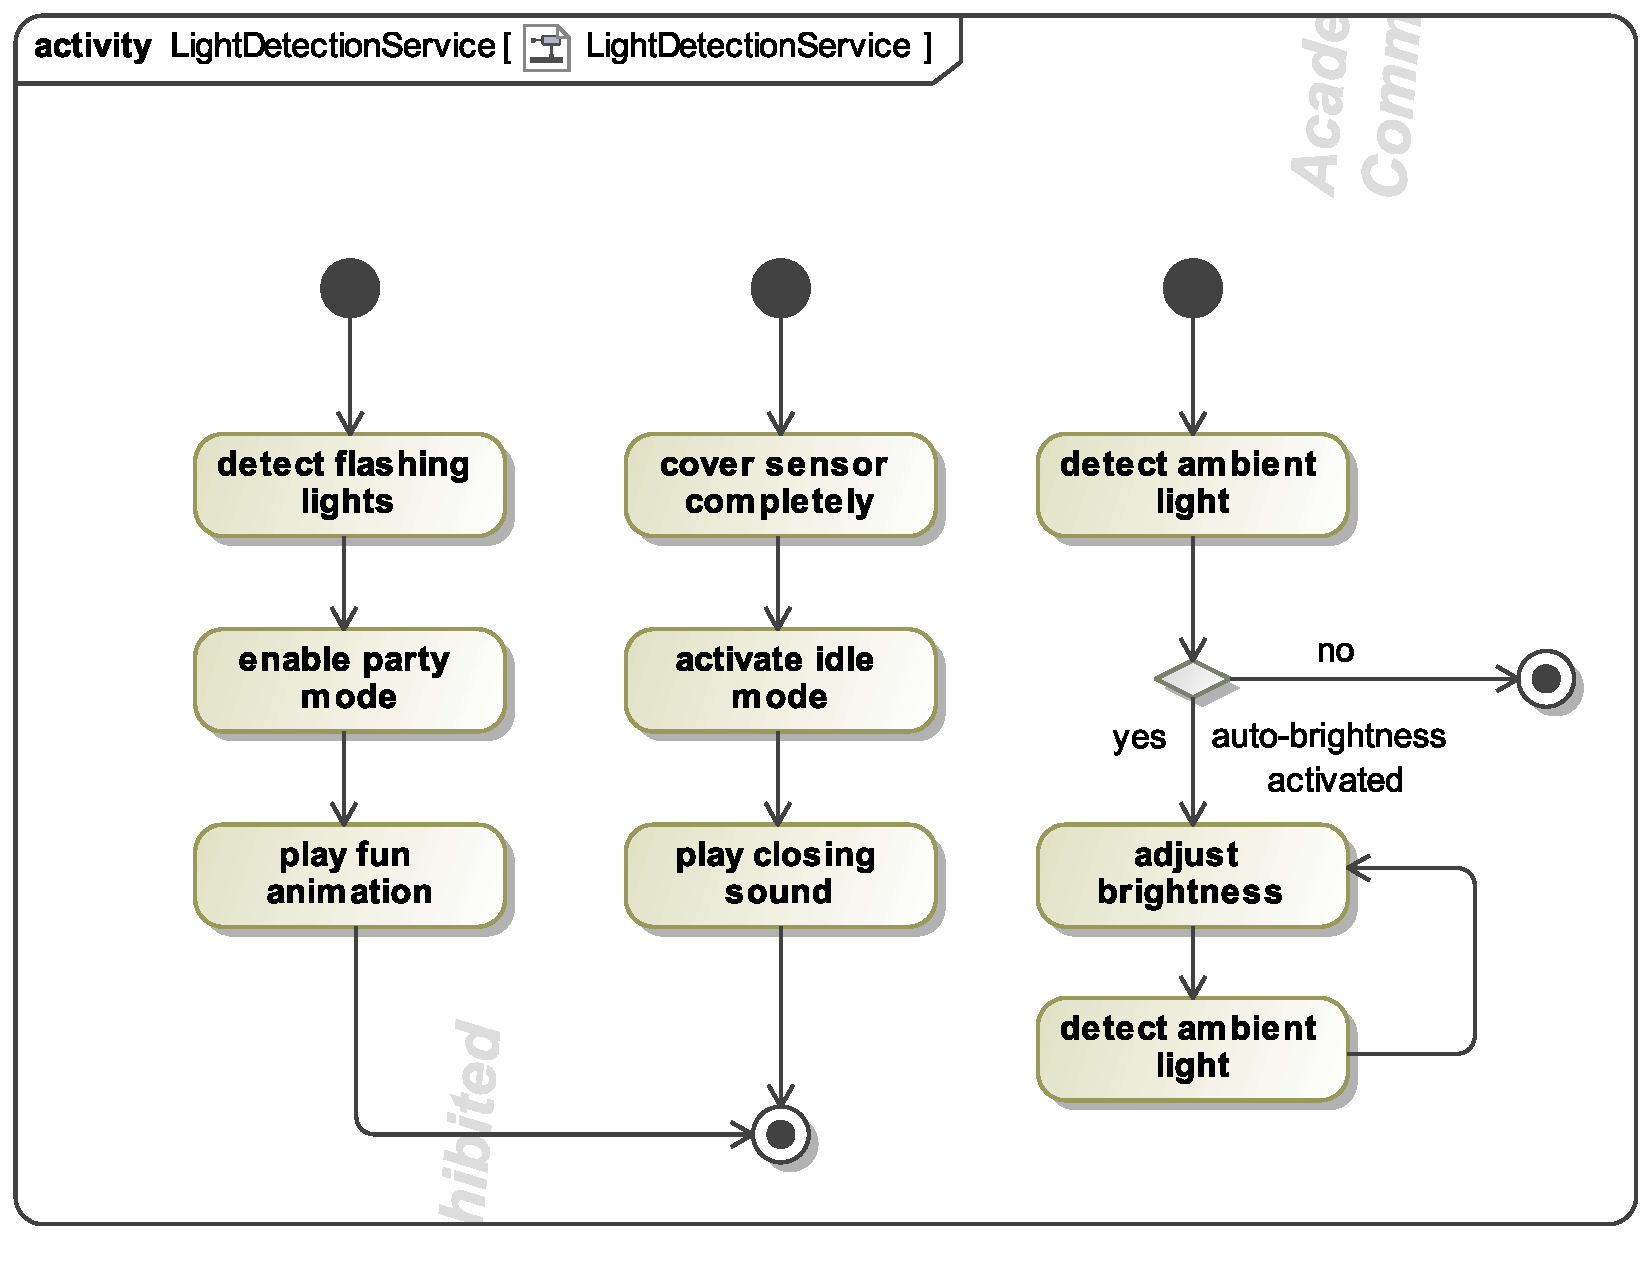
\includegraphics[width=\textwidth, angle=0]{Marc/light/LightDetectionServiceActivity.pdf}
		\end{figure}
		\clearpage
		\begin{figure}[h!]
			\centering
			\captionsetup{labelformat=empty}
			\caption{UseCase Diagram - light detection for brightness (light sensor)}
		    	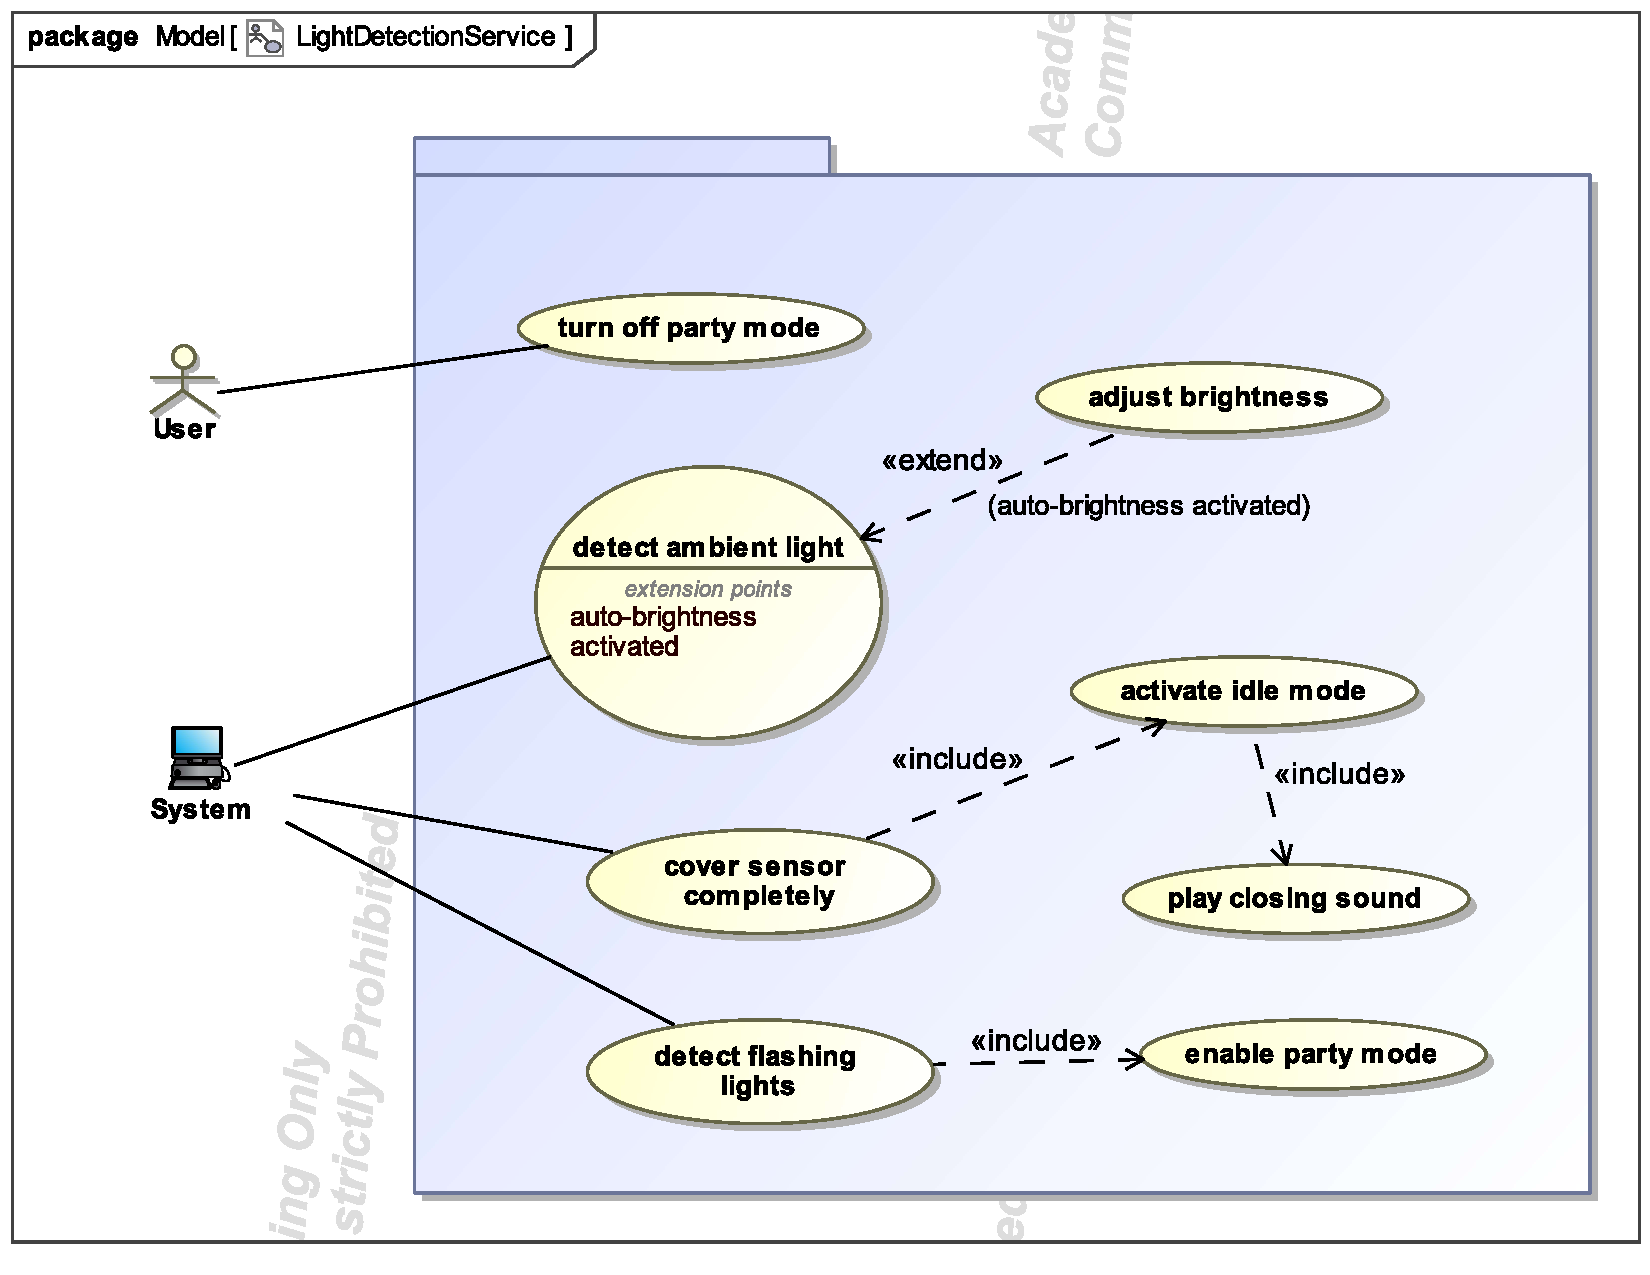
\includegraphics[width=\textwidth, angle=0]{Marc/light/LightDetectionServiceUseCase.pdf}
		\end{figure}
		\clearpage
		\begin{figure}[h!]
			\centering
			\captionsetup{labelformat=empty}
			\caption{Sequence Diagram - light detection for brightness (light sensor)}
		    	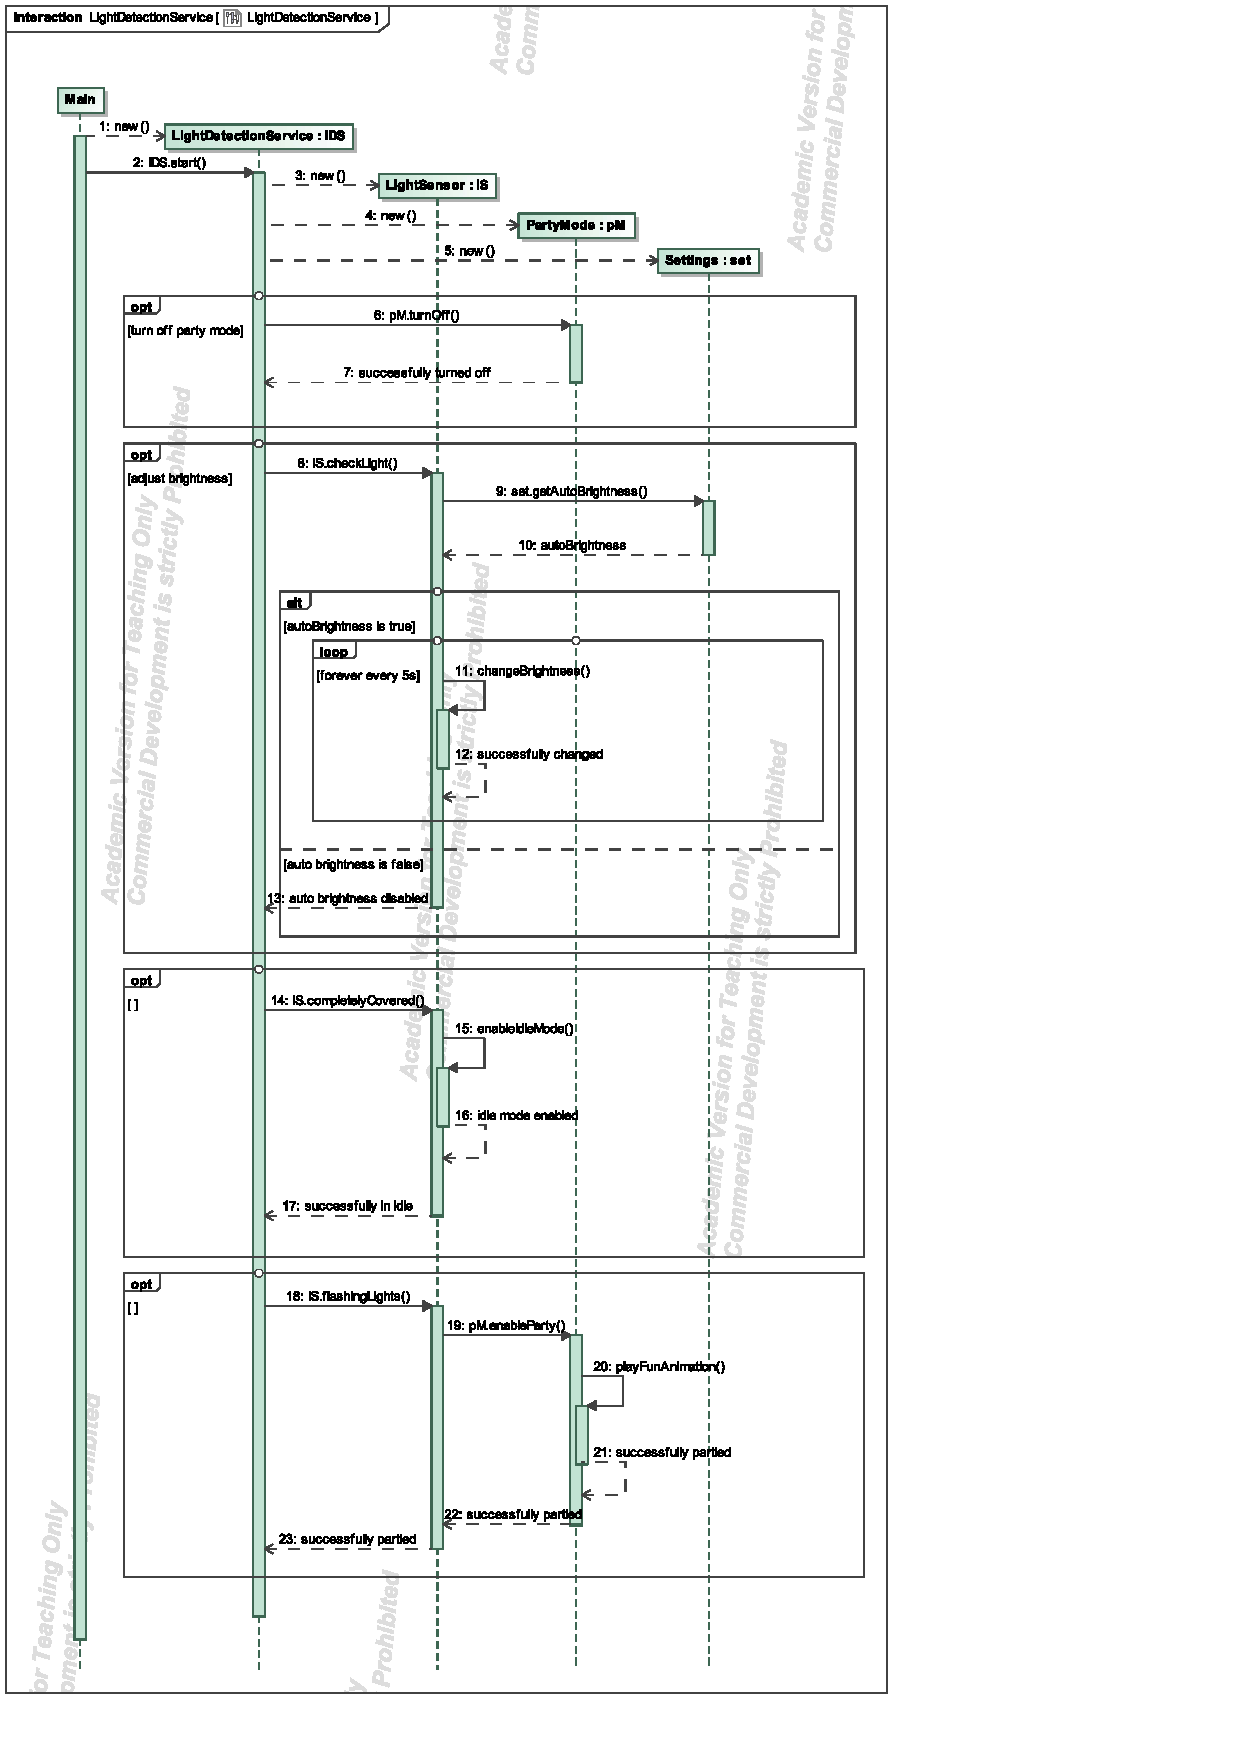
\includegraphics[scale=0.78, angle=0]{Marc/light/LightDetectionServiceSequence.pdf}
		\end{figure}
		\clearpage
		\begin{figure}[h!]
			\centering
			\captionsetup{labelformat=empty}
			\caption{Class Diagram - light detection for brightness (light sensor)}
		    	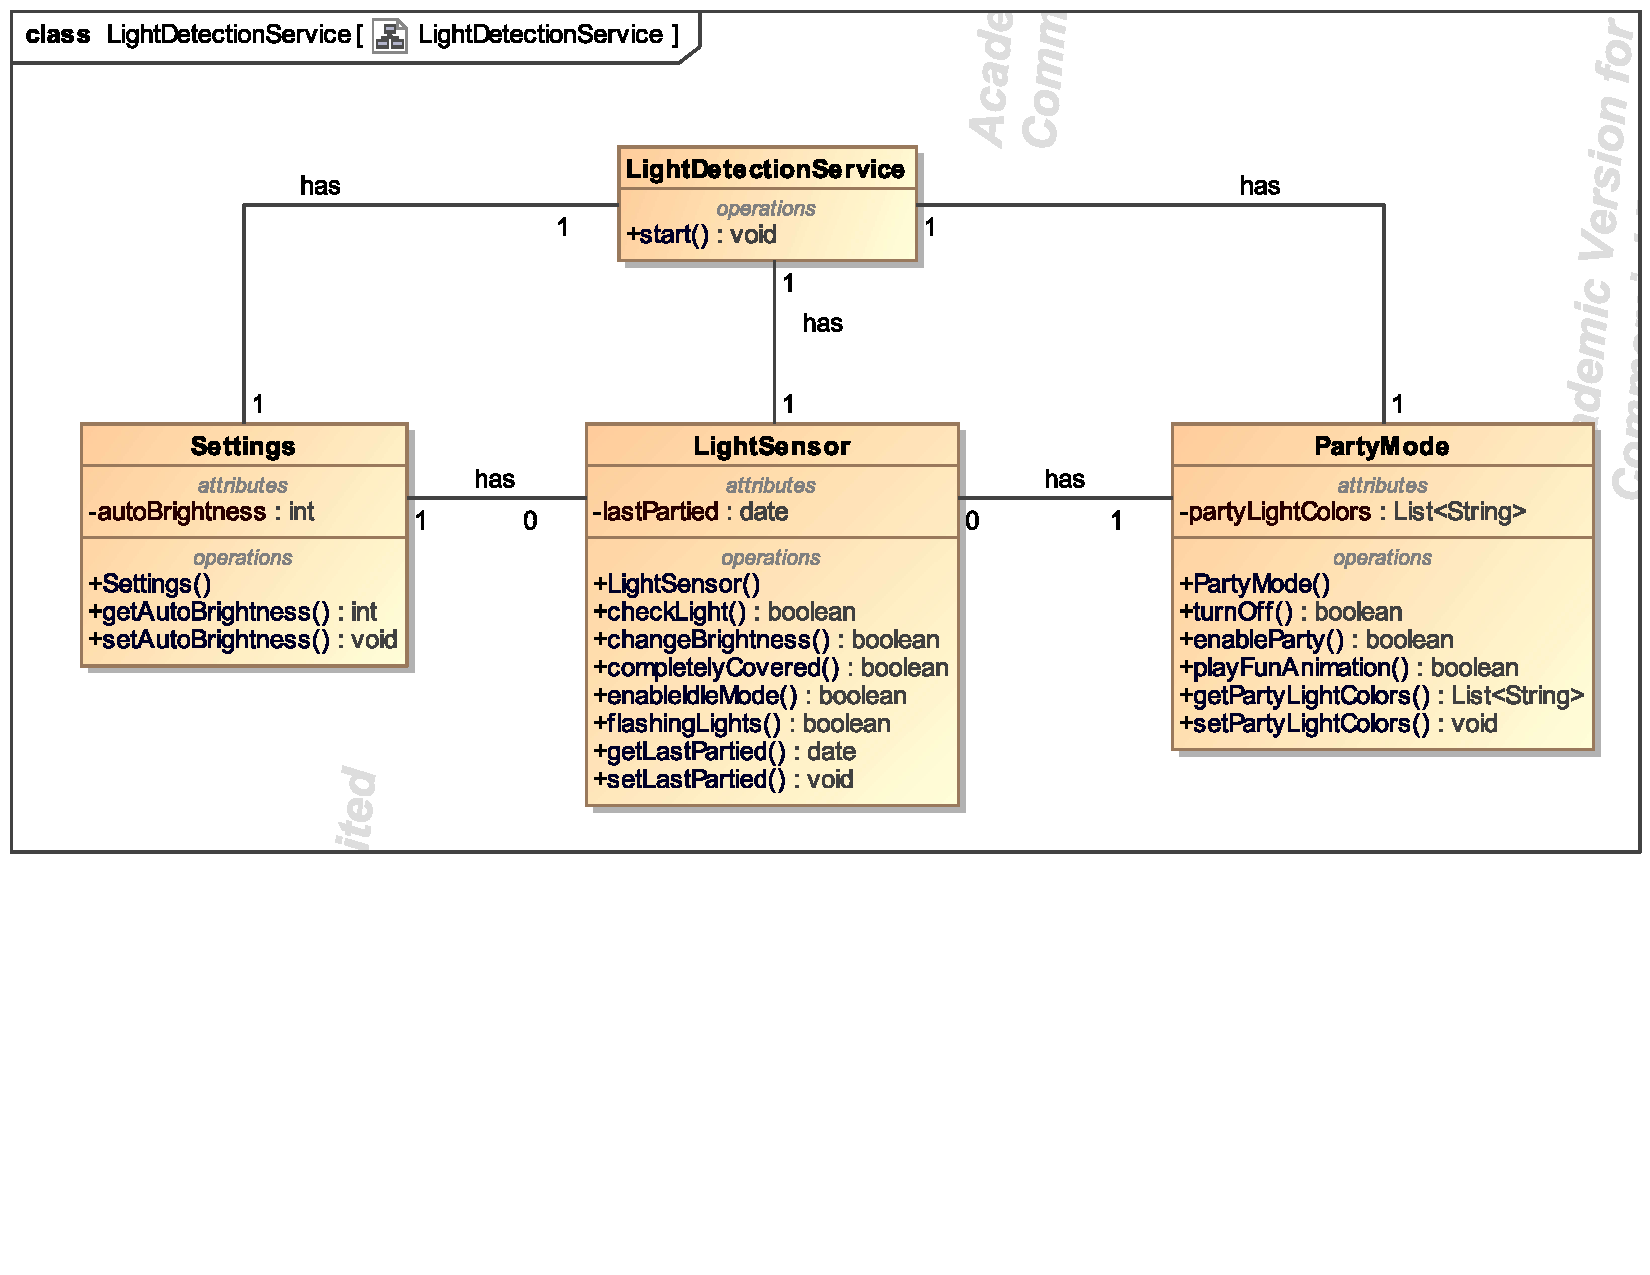
\includegraphics[width=\textwidth, angle=0]{Marc/light/LightDetectionServiceClass.pdf}
		\end{figure}
		\clearpage	

\section{Stefan Nguyen}

\subsection{Requirement 3: Display Heart Rate on Smartwatch}
	\begin{center}
		\begin{tabularx}{1.0\textwidth}{|>{\raggedright\arraybackslash}p{0.2\textwidth}|>{\raggedright\arraybackslash}X|}
			\hline
			Name             & Display Heart Rate on Smartwatch \\ \hline
			ID               & 3 \\ \hline
			Business Value   & Medium \\ \hline
			Description      & User can look at their herat beat data on the smartwatch \\ \hline
			Trigger          & Click app icon from "health app" on smartwatch display, and then enter section "heart beat" \\ \hline
			Actors           & User, Health data app, Heartbeat sensor \\ \hline
			Pre-conditions   & Smartwatch turned on \\ \hline
			Post-conditions  & User receives information about his health data \\ \hline
			Basic Flow       & \\ \hline
							Description & This is the main scenario where the user already has a valid account and password \\ \hline
							Actions & \\ \hline
							1 & The user opens the heartbeat app \\ \hline
							2 & The app presents the user current heart rate in real time \\ \hline
			Alternative Flow & A \\ \hline
							Description & Inaccurate sensoring of the heart beat \\ \hline
							Actions & \\ \hline
							1 & The app alerts the user about potential inaccuracy of the heart beat rate because of sensor issues. \\ \hline
							2 & The app guides the user through a recalibration of the sensor for accurate results.  \\ \hline
			Alternative Flow & B \\ \hline
							Description & App sensors an anomaly in the heartbeat pattern  \\ \hline
							Actions & \\ \hline
							1 & The app sends a push notification to the user that the sensors detected an irregular heart beat. \\ \hline
							2 & The app provides guidance and relaxation techniques to normalize the heart beat rate. \\ \hline
							3 & If the heart beat doesn't change the app gives the user the possibility to call medical service. \\ \hline
		\end{tabularx}
	\end{center}
	\paragraph{Functional requirements}
		\begin{itemize}
			\item The smartwatch should be able to display the user's current heart rate in real time when the application is active.
			\item If the heart rate doesn't return to the normal state, the user is able to call emergency. 
		\end{itemize}
		
	\paragraph{Non-functional requirements}
		\begin{itemize}
			\item The sensor must provide accurate readings within a specific tolerance e.g. +/- 2-3 heart beats per minute under normal condition. 
			\item The app displays the heart rate within specific time frames, so delays should be minimal
		\end{itemize}
		 \clearpage

	\begin{figure}[htbp]
		\textbf{Use Case Diagram - Display Heart Rate on Smartwatch}
		\centering
		\begin{subfigure}{\textwidth}
			\resizebox{\textwidth}{!}{\includesvg[]{Stefan/Display heart rate data on smartwatch/DisplayHeartRateDataOnSmartwatch_use_case_diagram.svg}}
			\caption{Use Case Diagram}
		\end{subfigure}
		\begin{subfigure}{\textwidth}
			The User has specific interactions for example he is able to review his heart rate on the history, he can also receive
			heart rate alerts which will include safety confirmation and extend if an emergency is needed. We can also set a limit of heart rate for example,
			if the user sets the limit to 140 bpm then he will get notified if we get passed that bpm. Next he can view the current heart rate on the smartwatch.
			The External health monitoring service can sensor the heart rate proceed its data and give the user personal insight of his heart rate. 
		\end{subfigure}
	\end{figure}
	\clearpage

	\begin{figure}[htbp]
		\textbf{Activity Diagram - Display Heart Rate on Smartwatch}
		\centering
		\begin{subfigure}{\textwidth}
			\resizebox{\textwidth}{!}{\includesvg[]{Stefan/Display heart rate data on smartwatch/DisplayHeartRateDataOnSmartwatch_activity_diagram.svg}}
			\caption{Activity Diagram}
		\end{subfigure}
		\begin{subfigure}{\textwidth}
			Inside the Activity Diagram we start sensor the heart rate and proceed the data. Then with the given analysis it checks the 
			heart rate from the user. If its not fine we prepare an alert and send the user a safety confirmation. If its needed then we call an ambulance. If not 
			we can display the heartbeat data on the smartwatch. Then the user has a variety of options inside the smartwatch, e.g. 
			view current heart rate or the history of the past analysis or even receive personal insight of the heart rate. 
		\end{subfigure}
	\end{figure}

	\clearpage
	\begin{figure}[htbp]
		\textbf{Class Diagram - Display Heart Rate on Smartwatch}
		\centering
		\begin{subfigure}{\textwidth}
			\resizebox{\textwidth}{!}{\includesvg[]{Stefan/Display heart rate data on smartwatch/DisplayHeartRateDataOnSmartwatch_class_diagram.svg}}
			\caption{Class Diagram}
		\end{subfigure}
		\begin{subfigure}{\textwidth}
			Inside the Class Diagram we check the data from the User because height, weight or even age does play an important factor
			for the heart rate analysis. Next we sensor the heart rate from the user and proceed the data. For that we use a directional 
			association since we do the operation once, and the multiplicity stays 1 because we only use 1 sensor. Inside the process data we check for 
			the current heart rate. Last but not least, we display the data and the user is able to show the completed heart rate 
			analysis. 
		\end{subfigure}
	\end{figure}
	\clearpage

	\begin{figure}[htbp]
		\textbf{Sequence Diagram - Display Heart Rate on Smartwatch}
		\centering
		\begin{subfigure}{\textwidth}
			\resizebox{\textwidth}{!}{\includesvg[]{Stefan/Display heart rate data on smartwatch/DisplayHeartRateDataOnSmartwatch_sequence_diagram.svg}}
			\caption{Sequence Diagram}
		\end{subfigure}
		\begin{subfigure}{\textwidth}
			Inside the Main we get the profile from the user and read the heartRate with the Sensor. Next we proceed the data and check 
			if a safety confirmation is needed. If yes we do an emergency call and we contact for medical assistance. Else we can process 
			the data and prepare to display the data to the user. When we send the data to the user we also make sure to stop the sensoring and 
			the user is able to review the current heart rate analysis. 
		\end{subfigure}
	\end{figure}
	\clearpage
	\begin{figure}[htbp]
		\textbf{UI Prototype - Display Heart Rate on Smartwatch}
		\centering
		\begin{subfigure}{\textwidth}
			\resizebox{\textwidth}{!}{\includesvg[]{Stefan/UI Prototypes/Heart rate.svg}}
		\end{subfigure}
		\begin{subfigure}{\textwidth}
		
		\end{subfigure}
	\end{figure}
	\clearpage

\subsection{Requirement 11: Environment Monitoring}
	\begin{center}
		\begin{tabularx}{1.0\textwidth}{|>{\raggedright\arraybackslash}p{0.2\textwidth}|>{\raggedright\arraybackslash}X|}
			\hline
			Name             & Environment monitoring \\ \hline
			ID               & 11 \\ \hline
			Business Value   & Low \\ \hline
			Description      & Tracks UV exposure, air quality, temperature in real time \\ \hline
			Trigger          & Typical event which adjusts the changes in real time \\ \hline
			Actors           & Environmental Sensor Array, which is responsible for capturing environmental data \\ \hline
			Pre-conditions   & Environmental sensors are operational and calibrated\\ \hline
			Post-conditions  & Displays the data in the smartwatch\\ \hline
			Basic Flow       & \\ \hline
							  Description & Detail each change in the environment monitoring system \\ \hline
							  Actions & \\ \hline
							  1 & activating the sensors \\ \hline
							  2 & capturing the data (e.g. temperature, UV, etc) \\ \hline
							  3 & processing data e.g. analysis or computations \\ \hline
							  4 & transfer data into smartwatch \\ \hline
							  5 & display data in smartwatch \\ \hline
			Alternative Flow & A \\ \hline
							  Description & Error capturing data (network, communication etc) \\ \hline
							  Actions & \\ \hline
							  1 & sensor fails to capture data \\ \hline
							  2 & fail, communication or network error in smartwatch or sensor \\ \hline
							  3 & Error capturing data / false data display information \\ \hline
			Alternative Flow & B \\ \hline
							  Description & Environmental sensor detect conditions which my threaten health conditions \\ \hline
							  Actions & \\ \hline
							  1 & sensor detects hazardous condition and flag it as highest priority \\ \hline
							  2 & sends push notification and warns the user \\ \hline
							  3 & displays the notification on the smartwatch and recommends actions (e.g. apply sunscreen, seek shelter, etc) \\ \hline
							  4 & user acknowledges the notification\\ \hline
							  5 & user doesn't acknowledge notification -> the system keeps sending notifications or warns the user \\ \hline
		\end{tabularx}
	\end{center}
	\paragraph{Functional requirements}
		\begin{itemize}
			\item The sensor should automatically activate to environment changes or updates.
			\item It needs to capture the environment data in real time.
		\end{itemize}
		
	\paragraph{Non-functional requirements}
		\begin{itemize}
			\item The display of the environment data on the smartwatch must be clear, intuitive and easily to understand. 
			\item Must optimize low power consumption to minimize impact to smartwatch battery life. 
		\end{itemize}
	
		\clearpage
	\begin{figure}[htbp]
		\textbf{Use Case Diagram - Environment Monitoring}
		\centering
		\begin{subfigure}{\textwidth}
			\resizebox{\textwidth}{!}{\includesvg[]{Stefan/Environment Monitoring/EnvironmentMonitoring_use_case_diagram.svg}}
			\caption{Use Case Diagram}
		\end{subfigure}
		\begin{subfigure}{\textwidth}
			The Environment Monitoring shows the use cases. The activity sensor sensors the environment and transmit
			proceeds the data and generate a safe monitoring notification. This tells the user the current environment e.g.
			temperature, UV exposure or more. If it comes to hazardous conditions it sends the user a notification and asks him 
			to either acknowledge or not. Next the activity sensor displays the data on the smartwatch and record or
			track any other incident reports. The user on the other hand can acknowledge the notification and look into
			history data and has an authentication. 
		\end{subfigure}
	\end{figure}
	\clearpage

	\begin{figure}[htbp]
		\textbf{Activity Diagram - Environment Monitoring}
		\centering
		\begin{subfigure}{\textwidth}
			\resizebox{\textwidth}{!}{\includesvg[]{Stefan/Environment Monitoring/EnvironmentMonitoring_activity_diagram.svg}}
			\caption{Activity Diagram}
		\end{subfigure}
		\begin{subfigure}{\textwidth}
			The activity diagram shows a walkthrough of the operations or activities that need to be done, 
			so it can monitor the environment. Firstly, it activates the sensor and collects all the environment 
			data and transmits/proceeds them. It later asks for safe monitoring to ensure that there are no incidents 
			like hazards or natural disasters. If the user clicks no then the system prepares the notification and 
			asks the user to acknowledge the alert. The alert shows tips or recommendations which need to be done, to 
			shorten the risk of endangering personal life. If the user doesn’t accept the notification then the system 
			keeps warning the user or keeps spamming alerts, else it displays the data with the notification.
		\end{subfigure}
	\end{figure}
	
	\clearpage
	\begin{figure}[htbp]
		\textbf{Class Diagram - Environment Monitoring}
		\centering
		\begin{subfigure}{\textwidth}
			\resizebox{\textwidth}{!}{\includesvg[]{Stefan/Environment Monitoring/EnvironmentMonitoring_class_diagram.svg}}
			\caption{Class Diagram}
		\end{subfigure}
		\begin{subfigure}{\textwidth}
			The UML shows the structure of the classes, how they interact with each other and what methods are 
			used later in the sequence diagram. For example, the Activity Sensor sends data to the process data 
			which is a unidirectional relation with 1. The activity sensor has methods like activate sensor, keep 
			monitoring and stop monitoring. The monitoring would work permanently while the smartwatch is on. The 
			process list has the notifications, hazardous condition and process data and uses the unidirectional 
			relation to the display. While the display formats the data to the smartwatch so that the user can access 
			the data and can see the outputted data. 
		\end{subfigure}
	\end{figure}
	\clearpage

	\begin{figure}[htbp]
		\textbf{Sequence Diagram - Environment Monitoring}
		\centering
		\begin{subfigure}{\textwidth}
			\resizebox{\textwidth}{!}{\includesvg[]{Stefan/Environment Monitoring/EnvironmentMonitoring_sequence_diagram.svg}}
			\caption{Sequence Diagram}
		\end{subfigure}
		\begin{subfigure}{\textwidth}
			The sensor diagram almost works the same way as the display heartbeat data. It activates the sensor, 
			does the process and checks for hazardous conditions in the environment and does the following alternative
			operations. Later it either sends a notification or outputs the data to the display of the smartwatch. 
			The small part of smartwatch on represents that the sensor works permanently and keeps monitoring until 
			the smartwatch is off. 
		\end{subfigure}
	\end{figure}
	\clearpage

\subsection{Requirement 23: Pay with Smartwatch}
	\begin{center}
		\begin{tabularx}{1.0\textwidth}{|>{\raggedright\arraybackslash}p{0.2\textwidth}|>{\raggedright\arraybackslash}X|}
			\hline
			Name             & Pay with Smartwatch \\ \hline
			ID               & 23 \\ \hline
			Business Value   & Low \\ \hline
			Description      & Allows users to make payments using their smartwatch connected to a digital wallet or bank account. \\ \hline
			Trigger          & User chooses to pay with a smartwatch within an app  \\ \hline
			Actors           & User, Payment System, Bank \\ \hline
			Pre-conditions   & smartwatch with payment capability, bank acount must be linked to digital wallet, the card reader supports the smartwatch payments \\ \hline
			Post-conditions  & process confirmed, receipt sent to user email, recorded to the transaction history \\ \hline
			Basic Flow       & \\ \hline
							Description & User completes the smartwatch transaction \\ \hline
							Actions & \\ \hline
							1 & Selects "Pay with Smartwatch" option within the app and reads with the card reader \\ \hline
							2 & User sees the amount to pay and confirms the payment  \\ \hline
							3 & Payment system processes the transaction with the user's bank or digital wallet \\ \hline
							4 & confirmation through the card reader and receipt sent to the users email \\ \hline
			Alternative Flow & A \\ \hline
							Description & Payment with smartwatch fails due to connectivity issues \\ \hline
							Actions & \\ \hline
							1 & User attempts to pay, but the smartwatch cant connect to the card reader \\ \hline
							2 & The card reader sends an error message \\ \hline
							3 & User resolves the issue or decides to pay with a different payment method \\ \hline
			Alternative Flow & B \\ \hline
							Description & Payment declined by the bank or digital wallet \\ \hline
							Actions & \\ \hline
							1 & User confirms the payment on the smartwatch \\ \hline
							2 & Payment system processes the transaction but receives an error due wrong password  \\ \hline
							3 & User retry entering password but still no result \\ \hline
							4 & Bank account blocks the card \\ \hline
							5 & User gets notified and needs to pay with a different payment method \\ \hline
		\end{tabularx}
	\end{center}
	\paragraph{Functional requirements}
		\begin{itemize}
			\item The smartwatch must provide an option for users to initiate a payment via app or interface. 
			\item The User should be able to review the payment amount and confirm the transaction directly to the smartwatch. 
		\end{itemize}
		
	\paragraph{Non-functional requirements}
		\begin{itemize}
			\item The payment process should be easy and require minimal steps to complete the transaction. 
			\item The payment should have high reliability with high success rate for transaction and minimal downtime. 
		\end{itemize}
		\clearpage

	\begin{figure}[htbp]
		\textbf{Use Case Diagram - Pay with Smartwatch}
		\centering
		\begin{subfigure}{\textwidth}
			\resizebox{\textwidth}{!}{\includesvg[]{Stefan/Pay with Smartwatch/PayWithSmartwatch_use_case_diagram.svg}}
			\caption{Use Case Diagram}
		\end{subfigure}
		\begin{subfigure}{\textwidth}
			The Use Case Diagram describes the different connection and actions the user can do within the smartwatch. For example, 
			the user is able to pay with the smartwatch. After it reads the smartwatch in the card reader it verifies the card and 
			either complete the transaction or cancel the transaction. If the transaction completes the user gets a receipt or an 
			email which confirms the payment. In addition the user is able to manage his bank accounts inside the smartwatch application. 
		\end{subfigure}
	\end{figure}
	\clearpage

	\begin{figure}[htbp]
		\textbf{Activity Diagram - Pay with Smartwatch}
		\centering
		\begin{subfigure}{\textwidth}
			\resizebox{\textwidth}{!}{\includesvg[]{Stefan/Pay with Smartwatch/PayWithSmartwatch_activity_diagram.svg}}
			\caption{Activity Diagram}
		\end{subfigure}
		\begin{subfigure}{\textwidth}
			The Activity Diagram describes the process of actions. For example the user holds his smartwatch with the digital card
			to a card reader and the card reader verifies if the card exists or does not. If the card doesn't exists it notifies
			the user that the card is invalid. Else we proceed to the bank account and the user should enter the password. If the 
			password is wrong it requests to enter the password again. After 3 tries it should automatically block the user. Else the 
			cash has been successfully transferred and the user can complete the transaction. 
		\end{subfigure}
	\end{figure}
	\clearpage

	\begin{figure}[htbp]
		\textbf{Class Diagram - Pay with Smartwatch}
		\centering
		\begin{subfigure}{\textwidth}
			\resizebox{\textwidth}{!}{\includesvg[]{Stefan/Pay with Smartwatch/PayWithSmartwatch_class_diagram.svg}}
			\caption{Class Diagram}
		\end{subfigure}
		\begin{subfigure}{\textwidth}
			The Class Diagram shows the interactions and relationships to each single process. For example, the User is
			able to create an account and register himself. Then it has a directional association to the proceed Data. Thats
			where the card is being checked, whether it exists or not. If it exists we simply go to the bank account and check 
			for the password and get the receipt that the transaction was successful. If there is a case when the password is 
			incorrect we simply ask the user to retry. If the retries all failed or the user decides to pay with a different 
			payment method we need to stop the process. 
		\end{subfigure}
	\end{figure}
	\clearpage
	\begin{figure}[htbp]
		\textbf{Sequence Diagram - Pay with Smartwatch}
		\centering
		\begin{subfigure}{\textwidth}
			\resizebox{\textwidth}{!}{\includesvg[]{Stefan/Pay with Smartwatch/PayWithSmartwatch_sequence_diagram.svg}}
			\caption{Sequence Diagram}
		\end{subfigure}
		\begin{subfigure}{\textwidth}
			Inside the Sequence Diagram we have a Main which opens the smartwatch. Then the user checks the digital card with the 
			card reader if it exists or not. If it doesn't we simply stop the program. Else we can just check if its vaild and request the 
			user to enter the password. If the password is correct we get the receipt and the transaction message. If we might occur to incorrect 
			password we have 2 more retries and if those 2 failed as well we stop the program if not we can get the receipt and the transaction
			message. 
		\end{subfigure}
	\end{figure}
	\clearpage
	\begin{figure}[htbp]
		\textbf{UI Prototype - Pay with Smartwatch}
		\centering
		\begin{subfigure}{\textwidth}
			\resizebox{\textwidth}{!}{\includesvg[]{Stefan/UI Prototypes/Wallet pay.svg}}
		\end{subfigure}
		\begin{subfigure}{\textwidth}
		
		\end{subfigure}
	\end{figure}
	\clearpage

\subsection{Requirement 24: Tips for using the Smartwatch}
	\begin{center}
		\begin{tabularx}{1.0\textwidth}{|>{\raggedright\arraybackslash}p{0.2\textwidth}|>{\raggedright\arraybackslash}X|}
			\hline
			Name             & Tips for using the Smartwatch \\ \hline
			ID               & 24 \\ \hline
			Business Value   & Low \\ \hline
			Description      & Provides the user with helpful tips and guidance throughout the smartwatch \\ \hline
			Trigger          & User request tips and help with the smartwatch interface or associated app \\ \hline
			Actors           & User, Smartwatch, Companion smartwatch app \\ \hline
			Pre-conditions   & Smartwatch connected with phone, needs basic knowledge for the usage of the smartwatch \\ \hline
			Post-conditions  & User receives helpful tips and feels more confident using the smartwatch, engagement with the features increased \\ \hline
			Basic Flow       & \\ \hline
							Description & The user accesses and navigates through the tips inside the smartwatch application \\ \hline
							Actions & \\ \hline
							1 & User opens the tips feature and see the companion smartphone app \\ \hline
							2 & Browse through different categories like, fitness help or functionality throughout the watch \\ \hline
							3 & Selects the option \\ \hline
							4 & Enhance the smartwatch usage \\ \hline
			Alternative Flow & A \\ \hline
							Description & Connectivity error or fail opening the tips application \\ \hline
							Actions & \\ \hline
							1 & User attempts to access the tips application, but an error appeared due to connectivity errors. \\ \hline
							2 & Smartwatch prompts the user to check the internet connection  \\ \hline
							3 & User resolves the issue and can successfully enter the tips application \\ \hline
			Alternative Flow & B \\ \hline
							Description & User requests specific tips through a voice command, but the smartwatch does not recognize the command.  \\ \hline
							Actions & \\ \hline
							1 & User gives a voice command requesting tips on a specific feature \\ \hline
							2 & The smartwatch fails to recognize the command and asks the user to try again \\ \hline
							3 & User repeats the command with clearer pronunciation \\ \hline
							4 & If the smartwatch still fails to recognize the command, it asks to type the request \\ \hline
							5 & User types the request, and the smartwatch displays the relevant tips \\ \hline
		\end{tabularx}
	\end{center}
	\paragraph{Functional requirements}
		\begin{itemize}
			\item The users should easily access the repository of tips and guidance directly from the smartwatch. 
			\item User's should be able to search for specific tips using keywords or phrases. 
		\end{itemize}
		
	\paragraph{Non-functional requirements}
		\begin{itemize}
			\item The Scalability needs to be good, so that it can handle an increasing number of tips. 
			\item The Content Quality for using the Tips application needs to be accurate and easy to follow / understand. 
		\end{itemize}
		\clearpage

	\begin{figure}[htbp]
		\textbf{Use Case Diagram - Tips for using the Smartwatch}
		\centering
		\begin{subfigure}{\textwidth}
			\resizebox{\textwidth}{!}{\includesvg[]{Stefan/Tips for using the Smartwatch/TipsUsingTheSmartwatch_use_case_diagram.svg}}
			\caption{Use Case Diagram}
		\end{subfigure}
		\begin{subfigure}{\textwidth}
			The Use Case Diagram for the Tips for using the smartwatch should just enhance the guidance for the user. So that the 
			user knows the new features of the smartwatch and help him get to know it better. So the user has the option to see a 
			variety of tips e.g. maintaining the device, customize the watch faces, smart notification and much more. Then if the user
			wants to find a specific tip there is also a search bar. Finally, the user can give feature advices inside the smartwatch
		\end{subfigure}
	\end{figure}
	\clearpage
	\begin{figure}[htbp]
		\textbf{Activity Diagram - Tips for using the Smartwatch}
		\centering
		\begin{subfigure}{\textwidth}
			\resizebox{\textwidth}{!}{\includesvg[]{Stefan/Tips for using the Smartwatch/TipsUsingTheSmartwatch_activity_diagram.svg}}
			\caption{Activity Diagram}
		\end{subfigure}
		\begin{subfigure}{\textwidth}
			The Activity Diagram shows the process for using the tips application. It is required to open the smartwatch and 
			navigate to the application. Then the user has options. For example, he can open the preset of tips, else he can search
			for specific elements. If the element is not found we simply notify the user that it's not available. 
			If the user choose a tip for guidance we simply continue with reading the tip or else we can just close the process. 
		\end{subfigure}
	\end{figure}
	\clearpage

	\begin{figure}[htbp]
		\textbf{Class Diagram - Tips for using the Smartwatch}
		\centering
		\begin{subfigure}{\textwidth}
			\resizebox{\textwidth}{!}{\includesvg[]{Stefan/Tips for using the Smartwatch/TipsUsingTheSmartwatch_class_diagram.svg}}
			\caption{Class Diagram}
		\end{subfigure}
		\begin{subfigure}{\textwidth}
			For the Class Diagram we have 3 classes. The user, search bar and then the tips application. The User usually 
			has an id for this smartwatch an account is registered with a name. If the user decides to pick one of the presets
			it directs him/her to the tipsApplication, where he can read the advice. Else if he decides to search for an element 
			we can find it and directs us to the tipsApplication. 
		\end{subfigure}
	\end{figure}
	\clearpage

	\begin{figure}[htbp]
		\textbf{Sequence Diagram - Tips for using the Smartwatch}
		\centering
		\begin{subfigure}{\textwidth}
			\resizebox{\textwidth}{!}{\includesvg[]{Stefan/Tips for using the Smartwatch/TipsUsingTheSmartwatch_sequence_diagram.svg}}
			\caption{Sequence Diagram}
		\end{subfigure}
		\begin{subfigure}{\textwidth}
			The Sequence Diagram shows the process of the application. For example the user has the application opened. Then it can
			either teake the presets which directs us to the tips application and gets us the output. Or else we can search the element. 
			If we search for the element, we check if its found or not. If not then we simply say that the element is not found and close the application. 
			The other option is that the user found the tip and gets the output. 
		\end{subfigure}
	\end{figure}
	\clearpage


\end{document}
